%==============================================================================

\chapter{Function-to-Algorithm Mapping}
\label{sec:function_mapping}

Table~\ref{tab:function_mapping} provides the complete tracing from result directories to simulation scripts to core function implementations, enabling verification of the algorithmic descriptions in Appendix~\ref{sec:algorithms}.

\begin{table}[H]
\centering
\caption{Complete Function-to-Algorithm Mapping}
\label{tab:function_mapping}
\footnotesize
\begin{tabularx}{\textwidth}{@{}l l l X@{}}
\toprule
\textbf{Algo} & \textbf{Result Directory} & \textbf{Script} & \textbf{Core Function (Line)} \\
\midrule
\multirow{2}{*}{1} & RQ1a\_ground\_truth\_correctness/ & run\_rq1a\_ground\_truth\_judge.py & judge\_all\_edges\_serial \\
 & RQ1a\_corruption\_det\_correctness/ & :179 $\rightarrow$ run\_discovery\_experiment & (modules.py:4421) \\
\midrule
\multirow{2}{*}{2} & RQ1a\_ground\_truth\_citation/ & run\_rq1a\_ground\_truth\_judge.py & judge\_all\_edges\_with\_citations\_serial \\
 & RQ1a\_corruption\_det\_citation/ & :179 $\rightarrow$ run\_discovery\_experiment & (modules.py:5688) \\
\midrule
3 & RQ1a\_corruption\_detection\_*/ & run\_rq1\_phase1\_single\_corrupt.py:74 & \_corrupt\_relationships (modules.py:1748) \\
\midrule
4 & RQ1b\_correction\_*/ & run\_rq1b\_correction\_single.py:121 & correct\_edges\_serial (modules.py:7050) \\
\midrule
\multirow{4}{*}{5} & \multirow{4}{*}{(computed during generation)} & \multirow{4}{*}{via run\_discovery\_experiment} & compute\_avg\_nll (logit\_metrics.py:177) \\
 & & & compute\_min\_prob (:251) \\
 & & & compute\_max\_window\_entropy (:259) \\
 & & & get\_embedding\_local (:98) \\
\midrule
6 & RQ2\_uq\_hallucination\_detection/ & rq2\_ensemble\_classifier.py & train\_classifiers (:32) \\
7 & (see Algorithm~\ref{alg:citation_fetcher}) & modules.py & fetch\_citations\_with\_jina (:265) \\
8 & RQ3\_deep\_research\_validation/ & test\_deep\_research\_ground\_truth.py & DeepResearchManager (pydantic\_ai\_deepresearch.py:642) \\
\bottomrule
\end{tabularx}
\end{table}

\textbf{Internal Dispatch:} \texttt{run\_discovery\_experiment()} (modules.py:11264) dispatches to:
\begin{itemize}[noitemsep]
    \item Line 11731: \texttt{\_corrupt\_relationships()} when \texttt{corruption\_rate > 0}
    \item Line 11792: \texttt{judge\_all\_edges\_with\_citations\_serial()} when \texttt{judge\_edges=True}
    \item Line 11844: \texttt{correct\_edges\_serial()} when \texttt{run\_correction=True}
\end{itemize}


\chapter{Reproducibility}
\label{sec:reproducibility}

This appendix provides comprehensive information for replicating all experiments, including data availability, code locations, software environment specifications, and exact execution commands.

\begin{center}
\fbox{\parbox{0.95\textwidth}{
\textbf{Reproduction Scope.} A public reproduction snapshot is available at \url{https://github.com/NitaiNijholt/cld-hallucination-detection} (branch: \texttt{thesis-reproduction}). This repository supports \textbf{analysis reproduction}---regenerating all thesis figures and tables from the included experimental result datasets using the unified analysis pipelines. \textbf{Simulation/data-generation} (i.e., re-running the original experiments to produce new result datasets) requires the private platform repository (\texttt{CausalixAI/platform}, branch: \texttt{thesis-nitai}), which contains proprietary infrastructure and external API dependencies not included in the public snapshot.

Paths in this appendix reference the public reproduction repository structure unless otherwise noted. Execution scripts for simulation (Section~\ref{sec:execution_commands}, Tables~\ref{tab:exec_scripts}) are documented for completeness but require access to the private platform.
}}
\end{center}

\section{Data Availability}
\label{sec:data_availability}

\subsection{Ground Truth CLD Datasets}

The three ground truth CLD datasets used in all experiments are available in JSON format within the public reproduction repository:
\begin{verbatim}
final_runs/analysis_lib/data/ground_truth_clds/
\end{verbatim}

\noindent These JSON files contain edge definitions, variable sets, and context data extracted from the original literature-derived CLDs. The analysis scripts use these files to compute ground-truth labels (TP/FP/FN) for edge evaluation.

\begin{table}[H]
\centering
\caption{Ground Truth CLD Dataset Files}
\label{tab:gt_files}
\footnotesize
\begin{tabularx}{\textwidth}{@{}l c c l >{\raggedright\arraybackslash}X@{}}
\toprule
\textbf{Domain} & \textbf{Nodes} & \textbf{Edges} & \textbf{Source} & \textbf{Filename} \\
\midrule
Depressive Symptoms & 14 & 34 & \citet{uleman2024triangulation} & \texttt{Depressive\_symptoms\_...\_healthy\_adults.xlsx} \\
Social Norms & 10 & 12 & \citet{crielaard2020socialnorms} & \texttt{Social\_norms\_and\_obesity\_prevalence.xlsx} \\
Emergency Department & 34 & 66 & \citet{smeekes2023emergency} & \texttt{older\_persons\_ED\_...\_spreadsheet.xlsx} \\
\bottomrule
\end{tabularx}
\end{table}

Each Excel file contains: edge definitions (source/target), relationship polarity, causal motivations, scientific citations, and generation-time UQ metrics.

\subsection{Validation and Auxiliary Datasets}

\begin{table}[H]
\centering
\caption{Validation and Auxiliary Datasets}
\label{tab:validation_datasets}
\footnotesize
\begin{tabularx}{\textwidth}{@{}l l c X@{}}
\toprule
\textbf{Dataset} & \textbf{Used In} & \textbf{Size} & \textbf{Location} \\
\midrule
TruthfulQA~\cite{lin2022truthfulqa} & RQ1 Verification & 1,634 Q\&A pairs & \texttt{final\_runs/RQ1\_verification\_Truth\_QA/} \\
Physics CLDs (see below) & RQ1a Validation & 31 edges, 4 CLDs & \texttt{final\_runs/validation\_RQ1a\_physics\_clds/cld\_data\_files/} \\
Uleman's Alzheimer CLD & RQ1a Validation & 150 edges & \texttt{final\_runs/validation\_RQ1a\_ulemans\_external/} \\
Human Validation Set & RQ1a Validation & 72 edges & \texttt{final\_runs/RQ1\_human\_validation\_citation\_judge/} \\
RQ3 DR Validation & RQ3 Human Val. & 50 edges & \texttt{final\_runs/RQ3\_deep\_research\_validation/human\_validation/} \\
\bottomrule
\end{tabularx}
\end{table}

\subsubsection{Physics CLD Details.} Four physics-based CLDs were constructed for sanity-check validation, derived from well-established physical laws:

\begin{table}[H]
\centering
\caption{Physics CLD Validation Dataset}
\label{tab:physics_cld_dataset}
\footnotesize
\begin{tabularx}{\textwidth}{@{}l c c X@{}}
\toprule
\textbf{CLD} & \textbf{Nodes} & \textbf{Edges} & \textbf{Physical Laws / Sources} \\
\midrule
Thermostat Heating & 7 & 8 & Newton's Law of Cooling~\cite{newton1701scala}; First Law of Thermodynamics~\cite{clausius1850heat} \\
Predator-Prey & 6 & 8 & Lotka-Volterra equations~\cite{lotka1925elements,volterra1928fluctuations} \\
RC Circuit & 7 & 8 & Ohm's Law~\cite{ohm1827galvanische}; Kirchhoff's Laws~\cite{kirchhoff1845durchgang} \\
Water Tank & 6 & 7 & Pascal's Law~\cite{pascal1663equilibre}; Torricelli's Law~\cite{torricelli1644opera} \\
\midrule
\textbf{Total} & 26 & 31 & \\
\bottomrule
\end{tabularx}
\end{table}

\textbf{Construction process.} The physics CLDs were constructed as follows:
\begin{enumerate}[noitemsep]
    \item \textbf{Causal structure definition:} Variables and directed edges were derived from established physical laws (Newton's Law of Cooling~\cite{newton1701scala}, First Law of Thermodynamics~\cite{clausius1850heat}, Lotka-Volterra equations~\cite{lotka1925elements,volterra1928fluctuations}, Ohm's and Kirchhoff's Laws~\cite{ohm1827galvanische,kirchhoff1845durchgang}, Pascal's and Torricelli's Laws~\cite{pascal1663equilibre,torricelli1644opera}). Edge polarities (\texttt{POSITIVE}/\texttt{NEGATIVE}) follow directly from the mathematical relationships in each law.
    \item \textbf{Motivation generation:} For each edge, causal explanations (``motivations'') were authored in an interactive session with Claude 4.5 Opus~\cite{anthropic2025claude45opus}, among the best-benchmarked models at time of writing. The prompt pattern was: ``\textit{Write a motivation for the edge [Source] $\rightarrow$ [Target] with polarity [POSITIVE/NEGATIVE] based on [Physical Law]. Include the relevant equation and cite sources.}'' This interactive process ensured each motivation accurately reflected the underlying physics while remaining accessible.
    \item \textbf{Reference mapping:} Each edge was annotated with bibliographic references to seminal papers and standard textbooks. Post-processing scripts (\texttt{add\_urls\_to\_references.py}, \texttt{add\_supporting\_quotes.py}) enriched the references with URLs (where publicly accessible) and supporting quotes extracted from source texts.
    \item \textbf{Verification:} All motivations and supporting quotes were manually verified against source texts to ensure scientific accuracy. URLs were browser-verified for accessibility (\texttt{verify\_and\_fix\_urls.py}).
    \item \textbf{Data format:} Final JSON structure: \texttt{\{source, target, polarity, motivation, references[\{short\_citation, full\_citation, url, supporting\_quote\}]\}}. Converted to Excel format via \texttt{create\_thermostat\_excel.py}.
\end{enumerate}

\noindent\textbf{Reproducibility note.} The motivation text was authored interactively (not via automated script) to ensure scientific precision. To reproduce similar motivations, one can prompt any capable LLM with the edge structure and underlying physical law, then verify against authoritative sources. The complete authored motivations, references, and all post-processing scripts are provided for full transparency.

\noindent\textbf{Data locations.} JSON files: \texttt{final\_runs/validation\_RQ1a\_physics\_clds/Data/physics\_clds\_with\_references/*.json}; post-processing scripts: same directory; Excel export: \texttt{create\_thermostat\_excel.py}; pipeline documentation: \texttt{PIPELINE\_EXPLANATION.md}.

\subsection{Experiment Result Datasets by Research Question}

\begin{table}[H]
\centering
\caption{Experiment Result Datasets by Research Question}
\label{tab:experiment_datasets}
\footnotesize
\begin{tabularx}{\textwidth}{@{}l l c X@{}}
\toprule
\textbf{RQ} & \textbf{Experiment} & \textbf{Files} & \textbf{Location} \\
\midrule
\multirow{4}{*}{RQ1a} 
  & GT Lit Correctness & 27 & \texttt{final\_runs/RQ1a\_gt\_lit\_correctness/} \\
  & GT Lit Citation & 36 & \texttt{final\_runs/RQ1a\_gt\_lit\_citation/} \\
  & GT Synth Correctness & 27 & \texttt{final\_runs/RQ1a\_gt\_synth\_correctness/} \\
  & GT Synth Citation & 36 & \texttt{final\_runs/RQ1a\_gt\_synth\_citation/} \\
\midrule
\multirow{2}{*}{RQ1b}
  & Correction GT Synth & 27 & \texttt{final\_runs/RQ1b\_corrector\_experiment\_corruption\_*/} \\
  & Correction GT Lit & 27 & \texttt{final\_runs/RQ1b\_corrector\_experiment\_ground\_truth\_*/} \\
\midrule
RQ2 & UQ Metrics Analysis & 63 & \texttt{final\_runs/RQ2\_uq\_hallucination\_detection/} \\
\midrule
RQ3 & Deep Research & 285 edges & \texttt{final\_runs/RQ3\_deep\_research\_validation/} \\
\midrule
\multirow{3}{*}{Prelim.}
  & Generator Comparison & 9 & \texttt{final\_runs/prelim\_generator\_model\_comparison/} \\
  & Temperature Sensitivity & 45 & \texttt{final\_runs/prelim\_temperature\_sensitivity/} \\
  & Random Baseline & 3,000 & \texttt{final\_runs/prelim\_random\_baseline\_generator/} \\
\midrule
Sens. & Prompt Sensitivity & 4 exp. & \texttt{final\_runs/supp\_prompt\_sensitivity/} \\
\bottomrule
\end{tabularx}
\end{table}

\subsection{Final Experiment Results}

All experimental results are stored in the \texttt{final\_runs/} directory:

\begin{verbatim}
final_runs/
+-- reproduce_all_thesis_assets.py    [Master reproduction script]
+-- RQ1_unified_analysis.py           [RQ1 analysis pipeline]
+-- RQ2_unified_analysis.py           [RQ2 analysis pipeline]
+-- RQ3_unified_analysis.py           [RQ3 analysis pipeline]
+-- SUPP_unified_analysis.py          [Supplementary analyses]
+-- PRELIM_unified_analysis.py        [Preliminary analyses]
+-- create_thesis_figure_structure.py [Maps outputs to thesis paths]
+-- analysis_lib/                     [Self-contained analysis code]
|   +-- analyze_rq1a_*.py             [RQ1a analysis scripts]
|   +-- logit_metrics.py              [Embedding utilities]
|   +-- data/ground_truth_clds/       [Ground truth CLD JSON files]
+-- RQ1a_gt_lit_correctness/          [GT Lit - Correctness Judge]
|   +-- depressive/run_{1,2,3}/       [Per-CLD result files]
|   +-- emergency_department/run_{1,2,3}/
|   +-- social_norms/run_{1,2,3}/
+-- RQ1a_gt_lit_citation/             [GT Lit - Citation Judge]
+-- RQ1a_gt_synth_correctness/        [GT Synth - Correctness Judge]
+-- RQ1a_gt_synth_citation/           [GT Synth - Citation Judge]
+-- RQ1b_corrector_experiment_*/      [Corrector experiments (by prompt)]
+-- RQ2_uq_hallucination_detection/   [UQ metrics analysis]
+-- RQ3_deep_research_validation/     [Deep Research validation]
+-- validation_RQ1_truthfulqa_judge/  [TruthfulQA benchmark]
+-- validation_RQ1a_physics_clds/     [Physics CLD validation]
+-- validation_RQ1a_ulemans_external/ [Uleman's CLD validation]
+-- prelim_generator_model_comparison/    [Generator model selection]
+-- prelim_random_baseline_generator/     [Random graph baseline]
+-- prelim_temperature_sensitivity/       [Temperature sensitivity]
+-- supp_parallelization_benchmark/       [Parallelization speedup]
+-- supp_prompt_sensitivity/              [Prompt sensitivity]
+-- supp_time_cost_scaling/               [Time/cost scaling]
\end{verbatim}

\section{Code Availability}
\label{sec:code_availability}

\subsection{Experiment Execution Scripts}

\begin{table}[H]
\centering
\caption{Primary Experiment Execution Scripts}
\label{tab:exec_scripts}
\footnotesize
\begin{tabularx}{\textwidth}{@{}l X X@{}}
\toprule
\textbf{Experiment} & \textbf{Script} & \textbf{Dependencies} \\
\midrule
RQ1a Ground Truth & \texttt{run\_rq1a\_ground\_truth\_multirun.py} & \texttt{run\_rq1a\_ground\_truth\_judge.py} \\
RQ1a Corruption (Corr.) & \texttt{run\_rq1a\_corruption\_multirun.py} & \texttt{run\_corruption\_detection\_pipeline.sh} \\
RQ1a Corruption (Cit.) & \texttt{run\_rq1a\_corruption\_citation\_multirun.py} & \texttt{run\_rq1\_judge\_citations\_all\_3\_prompts.py} \\
RQ1b Corrector & \texttt{run\_rq1b\_correction\_multirun.py} & \texttt{run\_rq1b\_correction\_single.py} \\
Temperature Sensitivity & \texttt{run\_temperature\_sensitivity.py} & \texttt{modules.py} (run\_discovery\_experiment) \\
\bottomrule
\end{tabularx}
\end{table}

All execution scripts located in: \texttt{data\_science/parameter\_tuning\_experiments/}

\noindent\textit{See also: Table~\ref{tab:analysis_scripts} (analysis scripts) and Table~\ref{tab:final_runs_script_inventory} (complete script inventory).}

\subsection{Analysis Scripts}

\begin{table}[H]
\centering
\caption{Analysis and Evaluation Scripts}
\label{tab:analysis_scripts}
\footnotesize
\begin{tabularx}{\textwidth}{@{}l X@{}}
\toprule
\textbf{Analysis} & \textbf{Script Path} \\
\midrule
\multicolumn{2}{@{}l}{\textit{RQ1a: LLM-as-Judge}} \\
RQ1a Aggregate Analysis & \texttt{final\_runs/analysis\_lib/analyze\_rq1a\_aggregate\_enhanced.py} \\
RQ1a Ground Truth Analysis & \texttt{final\_runs/analysis\_lib/analyze\_rq1a\_ground\_truth\_enhanced.py} \\
Physics CLD Validation & \texttt{final\_runs/validation\_RQ1a\_physics\_clds/analyse\_physics\_cld\_results.py} \\
Physics CLD Test Runner & \texttt{final\_runs/validation\_RQ1a\_physics\_clds/run\_physics\_cld\_tests.py} \\
Uleman's Provider Comparison & \texttt{final\_runs/validation\_RQ1a\_ulemans\_external/judge\_citation\_providers.py} \\
TruthfulQA Verification & \texttt{final\_runs/RQ1\_verification\_Truth\_QA/runner/truthqa\_judge\_baseline\_correctness.py} \\
\midrule
\multicolumn{2}{@{}l}{\textit{RQ1b: Corrector}} \\
RQ1b Results Analysis & \texttt{final\_runs/RQ1b\_corrector\_ablation\_analysis/scripts/analyze\_corrector\_ablation.py} \\
\midrule
\multicolumn{2}{@{}l}{\textit{RQ2: UQ Metrics}} \\
RQ2 Master Report & \texttt{final\_runs/RQ2\_uq\_hallucination\_detection/rq2\_master\_report\_v2\_enhanced.py} \\
RQ2 Batch Analyser & \texttt{final\_runs/RQ2\_uq\_hallucination\_detection/rq2\_simple\_batch\_analyser.py} \\
\midrule
\multicolumn{2}{@{}l}{\textit{RQ3: Deep Research}} \\
RQ3 Unified Analysis & \texttt{final\_runs/RQ3\_deep\_research\_validation/rq3\_unified\_analysis.py} \\
RQ3 Statistical Tests & \texttt{final\_runs/RQ3\_deep\_research\_validation/rq3\_statistical\_test.py} \\
RQ3 Per-CLD Detection Rates & \texttt{final\_runs/RQ3\_deep\_research\_validation/rq3\_per\_cld\_detection\_rates.py} \\
RQ3 Enrichment Metrics & \texttt{final\_runs/RQ3\_deep\_research\_validation/compute\_enriched\_gt\_metrics.py} \\
RQ3 Human Validation & \texttt{final\_runs/RQ3\_deep\_research\_validation/scripts/enrichment\_extrapolation.py} \\
RQ3 Smart Trigger Analysis & \texttt{final\_runs/RQ3\_deep\_research\_validation/scripts/estimate\_smart\_trigger\_dr\_enrichment.py} \\
RQ3 Cost Efficiency Plot & \texttt{final\_runs/RQ3\_deep\_research\_validation/scripts/plot\_dr\_cost\_efficiency.py} \\
RQ3 Figure Generation & \texttt{final\_runs/RQ3\_deep\_research\_validation/generate\_figures.py} \\
RQ3 Edge Sampling & \texttt{final\_runs/RQ3\_deep\_research\_validation/scripts/sample\_edges\_for\_validation.py} \\
RQ3 Validation Tables & \texttt{final\_runs/RQ3\_deep\_research\_validation/scripts/generate\_validation\_distribution\_tables.py} \\
\midrule
\multicolumn{2}{@{}l}{\textit{Preliminary \& Validation}} \\
Generator Model Comparison & \texttt{final\_runs/prelim\_generator\_model\_comparison/analysis\_scripts/analyze\_generator\_models.py} \\
Random Baseline Analysis & \texttt{final\_runs/random\_baseline\_generator/compute\_random\_baseline.py} \\
Embedding Model Benchmark & \texttt{final\_runs/supp\_embedding\_benchmark/embedding\_benchmark\_real\_cld.py} \\
Power Analysis & \texttt{final\_runs/power\_analysis/compute\_power\_analysis.py} \\
\midrule
\multicolumn{2}{@{}l}{\textit{Cost \& Scaling Analysis}} \\
Complete Cost Analysis & \texttt{final\_runs/supp\_cost\_analysis/calculate\_all\_costs.py} \\
Per-Experiment Costs & \texttt{final\_runs/supp\_cost\_analysis/calculate\_costs\_by\_experiment.py} \\
Deep Research Costs & \texttt{final\_runs/supp\_cost\_analysis/compute\_dr\_costs.py} \\
Token Analysis & \texttt{final\_runs/supp\_token\_analysis\_rq1a/analyse\_output\_tokens\_tiktoken.py} \\
Time/Cost Scaling & \texttt{final\_runs/supp\_time\_cost\_scaling/aggregate\_time\_cost\_scaling.py} \\
Parallelization Benchmark & \texttt{final\_runs/supp\_parallelization\_benchmark/analysis\_scripts/analyze\_parallelization\_results.py} \\
\midrule
\multicolumn{2}{@{}l}{\textit{Sensitivity Analysis}} \\
Judge Prompt Sensitivity & \texttt{final\_runs/supp\_prompt\_sensitivity/analysis\_scripts/sensitivity\_analysis\_simple.py} \\
Corrector Prompt Sensitivity & \texttt{final\_runs/supp\_prompt\_sensitivity/analysis\_scripts/sensitivity\_analysis\_corrector.py} \\
Temperature Assumption Tests & \texttt{final\_runs/temperature\_sensitivity\_assumption\_tests.py} \\
\bottomrule
\end{tabularx}
\end{table}

\noindent\textit{See also: Table~\ref{tab:exec_scripts} (execution scripts) and Table~\ref{tab:final_runs_script_inventory} (complete script inventory).}

\subsection{Complete \texttt{final\_runs/} Script and Command Inventory}
\label{sec:final_runs_script_inventory}

To make the artefact set auditable end-to-end, Table~\ref{tab:final_runs_script_inventory} enumerates the key runnable Python scripts present under \texttt{final\_runs/} in the public reproduction repository, together with canonical invocations from the repository root.

\noindent\textbf{Note:} Some scripts listed (particularly those requiring external API calls or database connections) may require additional configuration not included in the public snapshot. The unified analysis entry points are the recommended entry points for reproduction.

\begin{table}[H]
\centering
\caption{Complete \texttt{final\_runs/} Script and Command Inventory}
\label{tab:final_runs_script_inventory}
\footnotesize
\resizebox{\textwidth}{!}{%
\begin{tabular}{@{}ll@{}}
\toprule
\textbf{Script} & \textbf{Canonical command (from repo root)} \\
\midrule
\multicolumn{2}{@{}l}{\textit{Unified analysis entry points}} \\
\texttt{final\_runs/reproduce\_all\_thesis\_assets.py} & \texttt{uv run python final\_runs/reproduce\_all\_thesis\_assets.py} \\
\texttt{final\_runs/RQ1\_unified\_analysis.py} & \texttt{uv run python final\_runs/RQ1\_unified\_analysis.py} \\
\texttt{final\_runs/RQ2\_unified\_analysis.py} & \texttt{uv run python final\_runs/RQ2\_unified\_analysis.py} \\
\texttt{final\_runs/RQ3\_unified\_analysis.py} & \texttt{uv run python final\_runs/RQ3\_unified\_analysis.py} \\
\texttt{final\_runs/SUPP\_unified\_analysis.py} & \texttt{uv run python final\_runs/SUPP\_unified\_analysis.py} \\
\texttt{final\_runs/PRELIM\_unified\_analysis.py} & \texttt{uv run python final\_runs/PRELIM\_unified\_analysis.py} \\
\texttt{final\_runs/VALIDATION\_unified\_analysis.py} & \texttt{uv run python final\_runs/VALIDATION\_unified\_analysis.py} \\
\midrule
\multicolumn{2}{@{}l}{\textit{Top-level utilities}} \\
\texttt{final\_runs/aggregate\_time\_cost\_scaling.py} & \texttt{python final\_runs/aggregate\_time\_cost\_scaling.py} \\
\texttt{final\_runs/retrieve\_effect\_sizes.py} & \texttt{python final\_runs/retrieve\_effect\_sizes.py} \\
\texttt{final\_runs/temperature\_sensitivity\_assumption\_tests.py} & \texttt{python final\_runs/temperature\_sensitivity\_assumption\_tests.py} \\
\midrule
\multicolumn{2}{@{}l}{\textit{RQ1: TruthfulQA verification}} \\
\texttt{final\_runs/RQ1\_verification\_Truth\_QA/runner/truthqa\_judge\_baseline\_correctness.py} & \texttt{python final\_runs/RQ1\_verification\_Truth\_QA/runner/truthqa\_judge\_baseline\_correctness.py} \\
\texttt{final\_runs/RQ1\_verification\_Truth\_QA/analysis\_script/recalculate\_metrics.py} & \texttt{python final\_runs/RQ1\_verification\_Truth\_QA/analysis\_script/recalculate\_metrics.py} \\
\midrule
\multicolumn{2}{@{}l}{\textit{RQ1a validation: physics CLDs}} \\
\texttt{final\_runs/validation\_RQ1a\_physics\_clds/run\_physics\_cld\_tests.py} & \texttt{python final\_runs/validation\_RQ1a\_physics\_clds/run\_physics\_cld\_tests.py} \\
\texttt{final\_runs/validation\_RQ1a\_physics\_clds/analyse\_physics\_cld\_results.py} & \texttt{python final\_runs/validation\_RQ1a\_physics\_clds/analyse\_physics\_cld\_results.py} \\
\texttt{final\_runs/validation\_RQ1a\_physics\_clds/generate\_comparison\_table.py} & \texttt{python final\_runs/validation\_RQ1a\_physics\_clds/generate\_comparison\_table.py} \\
\texttt{final\_runs/validation\_RQ1a\_physics\_clds/generate\_retrieval\_comparison\_table.py} & \texttt{python final\_runs/validation\_RQ1a\_physics\_clds/generate\_retrieval\_comparison\_table.py} \\
\texttt{final\_runs/validation\_RQ1a\_physics\_clds/get\_avg\_scores.py} & \texttt{python final\_runs/validation\_RQ1a\_physics\_clds/get\_avg\_scores.py} \\
\texttt{final\_runs/validation\_RQ1a\_physics\_clds/cld\_data\_files/create\_thermostat\_excel.py} & \texttt{python final\_runs/validation\_RQ1a\_physics\_clds/cld\_data\_files/create\_thermostat\_excel.py} \\
\texttt{final\_runs/validation\_RQ1a\_physics\_clds/physics\_clds\_with\_references/add\_supporting\_quotes.py} & \texttt{python final\_runs/validation\_RQ1a\_physics\_clds/physics\_clds\_with\_references/add\_supporting\_quotes.py} \\
\texttt{final\_runs/validation\_RQ1a\_physics\_clds/physics\_clds\_with\_references/add\_urls\_to\_references.py} & \texttt{python final\_runs/validation\_RQ1a\_physics\_clds/physics\_clds\_with\_references/add\_urls\_to\_references.py} \\
\texttt{final\_runs/validation\_RQ1a\_physics\_clds/physics\_clds\_with\_references/show\_example.py} & \texttt{python final\_runs/validation\_RQ1a\_physics\_clds/physics\_clds\_with\_references/show\_example.py} \\
\texttt{final\_runs/validation\_RQ1a\_physics\_clds/physics\_clds\_with\_references/verify\_and\_fix\_urls.py} & \texttt{python final\_runs/validation\_RQ1a\_physics\_clds/physics\_clds\_with\_references/verify\_and\_fix\_urls.py} \\
\texttt{final\_runs/validation\_RQ1a\_physics\_clds/physics\_clds\_with\_references/verify\_urls.py} & \texttt{python final\_runs/validation\_RQ1a\_physics\_clds/physics\_clds\_with\_references/verify\_urls.py} \\
\midrule
\multicolumn{2}{@{}l}{\textit{RQ1a validation: Uleman's citation provider comparison}} \\
\texttt{final\_runs/validation\_RQ1a\_ulemans\_external/judge\_citation\_providers.py} & \texttt{python final\_runs/validation\_RQ1a\_ulemans\_external/judge\_citation\_providers.py} \\
\texttt{final\_runs/validation\_RQ1a\_ulemans\_external/compare\_jina\_vs\_scraper.py} & \texttt{python final\_runs/validation\_RQ1a\_ulemans\_external/compare\_jina\_vs\_scraper.py} \\
\midrule
\multicolumn{2}{@{}l}{\textit{RQ2: hallucination detection (UQ metrics)}} \\
\texttt{final\_runs/RQ2\_uq\_hallucination\_detection/rq2\_simple\_batch\_analyser.py} & \texttt{python final\_runs/RQ2\_uq\_hallucination\_detection/rq2\_simple\_batch\_analyser.py} \\
\texttt{final\_runs/RQ2\_uq\_hallucination\_detection/rq2\_master\_report\_v2\_enhanced.py} & \texttt{python final\_runs/RQ2\_uq\_hallucination\_detection/rq2\_master\_report\_v2\_enhanced.py} \\
\midrule
\multicolumn{2}{@{}l}{\textit{RQ3: Deep Research analysis}} \\
\texttt{final\_runs/RQ3\_deep\_research\_validation/analysis\_scripts/rq3\_unified\_analysis.py} & \texttt{python ...rq3\_unified\_analysis.py} \\
\texttt{final\_runs/RQ3\_deep\_research\_validation/analysis\_scripts/analyze\_deep\_research\_results.py} & \texttt{python ...analyze\_deep\_research\_results.py} \\
\texttt{final\_runs/RQ3\_deep\_research\_validation/analysis\_scripts/rq3\_statistical\_test.py} & \texttt{python ...rq3\_statistical\_test.py} \\
\texttt{final\_runs/RQ3\_deep\_research\_validation/analysis\_scripts/generate\_figures.py} & \texttt{python ...generate\_figures.py} \\
\texttt{final\_runs/RQ3\_deep\_research\_validation/analysis\_scripts/enrichment\_extrapolation.py} & \texttt{python ...enrichment\_extrapolation.py} \\
\texttt{final\_runs/RQ3\_deep\_research\_validation/analysis\_scripts/plot\_dr\_cost\_efficiency.py} & \texttt{python ...plot\_dr\_cost\_efficiency.py} \\
\midrule
\multicolumn{2}{@{}l}{\textit{Cost, scaling, and diagnostics}} \\
\texttt{final\_runs/supp\_cost\_analysis/calculate\_all\_costs.py} & \texttt{python final\_runs/supp\_cost\_analysis/calculate\_all\_costs.py} \\
\texttt{final\_runs/supp\_cost\_analysis/calculate\_costs\_by\_experiment.py} & \texttt{python final\_runs/supp\_cost\_analysis/calculate\_costs\_by\_experiment.py} \\
\texttt{final\_runs/supp\_cost\_analysis/calculate\_experiment\_costs.py} & \texttt{python final\_runs/supp\_cost\_analysis/calculate\_experiment\_costs.py} \\
\texttt{final\_runs/supp\_cost\_analysis/calculate\_costs\_max\_edges.py} & \texttt{python final\_runs/supp\_cost\_analysis/calculate\_costs\_max\_edges.py} \\
\texttt{final\_runs/supp\_cost\_analysis/analyse\_token\_and\_call\_stats.py} & \texttt{python final\_runs/supp\_cost\_analysis/analyse\_token\_and\_call\_stats.py} \\
\texttt{final\_runs/supp\_cost\_analysis/analyse\_output\_tokens\_tiktoken.py} & \texttt{python final\_runs/supp\_cost\_analysis/analyse\_output\_tokens\_tiktoken.py} \\
\texttt{final\_runs/supp\_cost\_analysis/compute\_dr\_costs.py} & \texttt{python final\_runs/supp\_cost\_analysis/compute\_dr\_costs.py} \\
\texttt{final\_runs/supp\_cost\_analysis/generate\_table21\_scaling\_summary.py} & \texttt{python final\_runs/supp\_cost\_analysis/generate\_table21\_scaling\_summary.py} \\
\texttt{final\_runs/supp\_token\_analysis\_rq1a/analyse\_output\_tokens\_tiktoken.py} & \texttt{python final\_runs/supp\_token\_analysis\_rq1a/analyse\_output\_tokens\_tiktoken.py} \\
\texttt{final\_runs/supp\_time\_cost\_scaling/aggregate\_time\_cost\_scaling.py} & \texttt{python final\_runs/supp\_time\_cost\_scaling/aggregate\_time\_cost\_scaling.py} \\
\texttt{final\_runs/supp\_time\_cost\_scaling/collect\_corrector\_timing.py} & \texttt{python final\_runs/supp\_time\_cost\_scaling/collect\_corrector\_timing.py} \\
\midrule
\multicolumn{2}{@{}l}{\textit{Sensitivity, benchmarks, and baselines}} \\
\texttt{final\_runs/supp\_prompt\_sensitivity/analysis\_scripts/sensitivity\_analysis\_simple.py} & \texttt{python final\_runs/supp\_prompt\_sensitivity/analysis\_scripts/sensitivity\_analysis\_simple.py} \\
\texttt{final\_runs/supp\_prompt\_sensitivity/analysis\_scripts/sensitivity\_analysis\_corrector.py} & \texttt{python final\_runs/supp\_prompt\_sensitivity/analysis\_scripts/sensitivity\_analysis\_corrector.py} \\
\texttt{final\_runs/supp\_prompt\_sensitivity/analysis\_scripts/sensitivity\_analysis\_simple\_rm\_anova.py} & \texttt{python final\_runs/supp\_prompt\_sensitivity/analysis\_scripts/sensitivity\_analysis\_simple\_rm\_anova.py} \\
\texttt{final\_runs/supp\_prompt\_sensitivity/analysis\_scripts/sensitivity\_analysis\_corrector\_rm\_anova.py} & \texttt{python final\_runs/supp\_prompt\_sensitivity/analysis\_scripts/sensitivity\_analysis\_corrector\_rm\_anova.py} \\
\texttt{final\_runs/supp\_parallelization\_benchmark/analysis\_scripts/analyze\_parallelization\_results.py} & \texttt{python ...analyze\_parallelization\_results.py} \\
\texttt{final\_runs/power\_analysis/compute\_power\_analysis.py} & \texttt{python final\_runs/power\_analysis/compute\_power\_analysis.py} \\
\texttt{final\_runs/prelim\_random\_baseline\_generator/analysis\_scripts/compute\_random\_baseline.py} & \texttt{python ...compute\_random\_baseline.py} \\
\texttt{final\_runs/supp\_embedding\_benchmark/embedding\_benchmark\_real\_cld.py} & \texttt{python ...embedding\_benchmark\_real\_cld.py} \\
\texttt{final\_runs/prelim\_generator\_model\_comparison/analysis\_scripts/analyze\_generator\_models.py} & \texttt{python ...analyze\_generator\_models.py} \\
\bottomrule
\end{tabular}%
}% end resizebox
\end{table}

\noindent\textit{See also: Table~\ref{tab:exec_scripts} (execution scripts) and Table~\ref{tab:analysis_scripts} (analysis scripts) for organised by-experiment views.}

\subsection{Prompt Configuration Files}

All prompts use three core variants (display names): \textit{\PromptBaseline} (direct instruction), \textit{\PromptMechanistic} (Bradford Hill criteria~\cite{shimonovich2020bradford}), and \textit{\PromptCoT} (chain-of-thought reasoning~\cite{kojima2022large}). In prompt configuration files, these correspond to the variant IDs \texttt{baseline}, \texttt{mechanistic}, and \texttt{cot}. Citation judges additionally include a fourth variant \textit{\PromptMechanisticLit} (variant ID \texttt{mech-lit}), which extends \PromptMechanistic{} with explicit literature grounding requirements.

\begin{table}[H]
\centering
\caption{Prompt Configuration Files (13 prompts: 2 judge tasks $\times$ 3 variants + 1 mech-lit + 1 corrector $\times$ 3 variants + 3 corruption)}
\label{tab:prompt_files}
\footnotesize
\begin{tabularx}{\textwidth}{@{}l l X@{}}
\toprule
\textbf{Task} & \textbf{Variants} & \textbf{File(s)} \\
\midrule
Judge-Correctness & baseline, mech, cot & \texttt{alternative\_prompts/prompts\_correctness\_\{baseline,mechanistic,cot\}.yaml} \\
Judge-Citation & baseline, mech, cot, mech-lit & \texttt{alternative\_prompts/prompts\_citation\_\{baseline,mechanistic,cot,mech\_lit\}.yaml} \\
Corrector & baseline, mech, cot & \texttt{corrector\_prompts.yaml} (variants within single file) \\
\midrule
Corruption & \multicolumn{2}{l}{\texttt{prompts\_Nitai\_C.yaml} (prompt IDs below):} \\
\quad -- motivation & (single) & \texttt{corruptor}: generates spurious but plausible motivation \\
\quad -- spurious edge & (single) & \texttt{generateSpuriousEdge}: NONE $\rightarrow$ false positive causal edge \\
\quad -- polarity flip & (single) & \texttt{generateFlippedPolarity}: POS $\leftrightarrow$ NEG with new motivation \\
\bottomrule
\end{tabularx}
\end{table}

\section{Software Environment}
\label{sec:software_env}

\begin{table}[H]
\centering
\caption{System and Runtime Environment}
\label{tab:system_env}
\footnotesize
\begin{tabular}{@{}ll@{}}
\toprule
\textbf{Component} & \textbf{Details} \\
\midrule
Hardware & ASUSTeK ROG Zephyrus G16 GU605CX\_GU605CX \\
CPU & Intel(R) Core(TM) Ultra 9 285H (16 cores, 16 logical processors) \\
GPU & NVIDIA GeForce RTX 5090 Laptop GPU (24463 MiB VRAM; driver 576.88) \\
System RAM & 64 GB DDR5 (8$\times$8 GB; 7467 MT/s configured) \\
Operating System & Ubuntu 24.04.2 LTS (WSL2; kernel 6.6.87.2-microsoft-standard-WSL2; Windows build 26100.7462) \\
Python Version & 3.10.18 (\texttt{.python-version}=3.10) \\
Package Manager & uv 0.8.3 \\
CUDA Version & 12.9 \\
\bottomrule
\end{tabular}
\end{table}

\subsection{Environment Installation}

All dependencies are managed using \texttt{uv}, a fast Python package manager with lockfile support for reproducible environments. To replicate the computational environment:

\begin{verbatim}
# Install uv (if not already installed)
curl -LsSf https://astral.sh/uv/install.sh | sh

# Clone public reproduction repository
git clone https://github.com/NitaiNijholt/cld-hallucination-detection.git
cd cld-hallucination-detection

# Sync exact versions from lockfile
uv sync

# Verify installation
uv run python -c "import pandas; import sklearn; print('OK')"
\end{verbatim}

\noindent The \texttt{uv.lock} file ensures deterministic dependency resolution, pinning all 104 packages to exact versions used during experiments. This dependency management approach is informed by principles from the Workflow for Open Reproducible Code in Science~\cite{vanlissa2021worcs}.

\subsection{Key Software Dependencies}

Full package dependencies with pinned versions are specified in \texttt{pyproject.toml}. Table~\ref{tab:software_citations} lists key software components with citations.

\begin{table}[H]
\centering
\caption{Key Software Dependencies and Citations}
\label{tab:software_citations}
\footnotesize
\begin{tabularx}{\textwidth}{@{}l l X@{}}
\toprule
\textbf{Package} & \textbf{Version} & \textbf{Citation} \\
\midrule
\multicolumn{3}{@{}l}{\textit{LLM APIs}} \\
OpenAI API & 1.107.3 & OpenAI (2023). GPT-4 Technical Report. arXiv:2303.08774 \\
Anthropic API & 0.61.0 & Anthropic (2024). Claude 3 Model Card \\
\midrule
\multicolumn{3}{@{}l}{\textit{Data Analysis}} \\
NumPy & 2.2.3 & \citep{harris2020numpy} \\
pandas & 2.2.3 & \citep{mckinney2010pandas} \\
SciPy & 1.15.3 & \citep{virtanen2020scipy} \\
\midrule
\multicolumn{3}{@{}l}{\textit{Machine Learning}} \\
scikit-learn & 1.7.2 & \citep{pedregosa2011sklearn} \\
imbalanced-learn & 0.14.0 & \citep{lemaitre2017imblearn} \\
\midrule
\multicolumn{3}{@{}l}{\textit{Visualisation}} \\
Matplotlib & 3.10.1 & \citep{hunter2007matplotlib} \\
seaborn & 0.13.2 & \citep{waskom2021seaborn} \\
\midrule
\multicolumn{3}{@{}l}{\textit{Graph \& Database}} \\
NetworkX & 3.4.2 & \citep{hagberg2008networkx} \\
Neo4j & 5.27.0 & \citep{robinson2013neo4j} \\
\midrule
\multicolumn{3}{@{}l}{\textit{LLM Integration}} \\
Pydantic & 2.11.7 & \citep{pydantic2024} \\
\midrule
\multicolumn{3}{@{}l}{\textit{Interactive Computing}} \\
Jupyter & 1.1.1 & \citep{kluyver2016jupyter} \\
\bottomrule
\end{tabularx}
\end{table}

\noindent Complete BibTeX citations for all software are available in the repository at \texttt{thesis/final\_thesis/software.bib}.

\section{Execution Commands}
\label{sec:execution_commands}

\subsection{Unified Analysis Entry Points (Single-command pipelines)}
\label{sec:unified_entry_points}

The directory \texttt{final\_runs/} contains three unified analysis entry points intended to reproduce the thesis results tables/figures with minimal manual orchestration:
\begin{verbatim}
cd <repo_root>

# RQ1 (TruthfulQA verification) + RQ1a (Judge) + RQ1b (Corrector)
uv run python final_runs/RQ1_unified_analysis.py \
  --run-dir final_runs/_runs/RQ1_<timestamp>

# RQ2 (UQ metrics + classifier pipeline + reporting)
uv run python final_runs/RQ2_unified_analysis.py \
  --run-dir final_runs/_runs/RQ2_<timestamp>

# RQ3 (Deep Research analysis + figures + validation artefacts)
uv run python final_runs/RQ3_unified_analysis.py \
  --run-dir final_runs/_runs/RQ3_<timestamp>
\end{verbatim}

For a complete directory-level overview, see \texttt{final\_runs/README\_DIRECTORY\_MAP.md}. The master reproduction script \texttt{reproduce\_all\_thesis\_assets.py} orchestrates all unified analyses and maps outputs to thesis figure paths.

\begin{center}
\fbox{\parbox{0.95\textwidth}{
\textbf{Note on Execution Scripts.} The subsections below (RQ1a--RQ3 execution commands) document the original simulation scripts used to generate experimental data. These scripts reside in the private platform repository (\texttt{data\_science/parameter\_tuning\_experiments/}) and are \textbf{not included} in the public reproduction snapshot. They are documented here for completeness and to enable full replication by examiners with platform access. For analysis reproduction using pre-computed result datasets, use the unified entry points above.
}}
\end{center}

\subsection{RQ1 Judge Verification (TruthfulQA)}
\label{sec:truthqa_verification}

Before evaluating judges on CLD-specific tasks, we verify baseline hallucination detection capability using the TruthfulQA benchmark. This sanity check helps ensure the evaluation pipeline behaves as expected before moving to the more domain-specific CLD setting; it does not, by itself, imply that any CLD-specific failures are purely domain-driven.

\begin{verbatim}
cd <repo_root>/final_runs/validation_RQ1_truthfulqa_judge/

# Run the TruthfulQA judge verification (baseline correctness prompt structure)
uv run python runner/truthqa_judge_baseline_correctness.py

# Optional: recompute summary metrics from a saved run JSON
# uv run python analysis_script/recalculate_metrics.py --input <path_to_results_json>
\end{verbatim}

\textbf{Script Location:} \texttt{final\_runs/RQ1\_verification\_Truth\_QA/runner/} \texttt{truthqa\_judge\_baseline\_correctness.py}

\textbf{Results Location:} \texttt{final\_runs/RQ1\_verification\_Truth\_QA/} (including \texttt{Data\_runs/})

\begin{table}[H]
\centering
\caption{TruthfulQA Verification Configuration}
\label{tab:truthqa_config}
\footnotesize
\begin{tabular}{@{}ll@{}}
\toprule
\textbf{Parameter} & \textbf{Value} \\
\midrule
Dataset & TruthfulQA (817 questions) \\
Samples & 1,634 (817 truthful + 817 hallucinated answers) \\
Judge Model & GPT-4.1 \\
Temperature & 0.0 \\
Seed & 42 \\
Prompt & Baseline correctness \\
Max Tokens & 250 \\
\bottomrule
\end{tabular}
\end{table}

\textbf{Output Files:}
\begin{itemize}[noitemsep]
    \item \texttt{truthfulqa\_results.json}: Per-sample verdicts
    \item \texttt{truthfulqa\_metrics.json}: Accuracy, precision, recall, F1
    \item \texttt{confusion\_matrix.png}: Classification confusion matrix
\end{itemize}

\subsection{RQ1a Ground Truth Experiments}
\label{sec:rq1a_execution}

\noindent\textit{[Requires private platform repository]}

\begin{verbatim}
# Private platform: data_science/parameter_tuning_experiments/
cd data_science/parameter_tuning_experiments/

# Correctness-based ground truth
python run_rq1a_ground_truth_multirun.py \
    --approach correctness \
    --output-dir ../../final_runs/RQ1a_gt_lit_correctness

# Citation-based ground truth
python run_rq1a_ground_truth_multirun.py \
    --approach citation \
    --output-dir ../../final_runs/RQ1a_gt_lit_citation
\end{verbatim}

\subsection{RQ1a Corruption Detection Experiments}

\begin{verbatim}
# Correctness-based corruption detection
python run_rq1a_corruption_multirun.py \
    --output-dir ../../final_runs/RQ1a_corrupted_correctness

# Citation-based corruption detection
python run_rq1a_corruption_citation_multirun.py \
    --output-dir ../../final_runs/RQ1a_corrupted_citation
\end{verbatim}

\begin{table}[H]
\centering
\caption{GT Synth Citation Judge Configuration (GPT-5-mini)}
\label{tab:gt_synth_citation_config}
\footnotesize
\begin{tabular}{@{}ll@{}}
\toprule
\textbf{Parameter} & \textbf{Value} \\
\midrule
Judge Model & GPT-5-mini \\
Temperature & 0.0 \\
Top-p & 1.0 \\
Approach & Citation-based judging \\
Parallelization & 10 workers \\
\midrule
\multicolumn{2}{@{}l}{\textit{Corruption}} \\
Corruption Rate & 30\% \\
Corruption Types & Motivation (spurious explanations), Structural (new edges, polarity flips) \\
\midrule
\multicolumn{2}{@{}l}{\textit{Dataset}} \\
CLDs & Depressive Symptoms, Social Norms, Emergency Department \\
Runs per CLD & 3 (seeds 1, 2, 3) \\
Prompt Variants & 4 (Baseline, CoT, Mechanistic, Mechanistic-Lit) \\
Total Experiments & 36 (3 CLDs $\times$ 3 runs $\times$ 4 prompts) \\
\bottomrule
\end{tabular}
\end{table}

\begin{table}[H]
\centering
\caption{RQ1a GT Lit Correctness Judge Configuration}
\label{tab:rq1a_gt_lit_correctness_config}
\footnotesize
\begin{tabular}{@{}ll@{}}
\toprule
\textbf{Parameter} & \textbf{Value} \\
\midrule
Judge Model & GPT-4.1 \\
Temperature & 0.0 \\
Seed & 42 \\
Approach & Correctness-based judging \\
Parallelization & 10 workers \\
Web Search & Disabled \\
\midrule
\multicolumn{2}{@{}l}{\textit{Dataset}} \\
CLDs & Depressive Symptoms, Social Norms, Emergency Department \\
Runs per CLD & 3 (seeds 10, 20, 30) \\
Prompt Variants & 3 (Baseline, CoT, Mechanistic) \\
Total Experiments & 27 (3 CLDs $\times$ 3 runs $\times$ 3 prompts) \\
\bottomrule
\end{tabular}
\end{table}

\begin{table}[H]
\centering
\caption{RQ1a GT Synth Correctness Judge Configuration}
\label{tab:rq1a_gt_synth_correctness_config}
\footnotesize
\begin{tabular}{@{}ll@{}}
\toprule
\textbf{Parameter} & \textbf{Value} \\
\midrule
Judge Model & GPT-4.1 \\
Temperature & 0.0 \\
Seed & 42 \\
Approach & Correctness-based judging \\
Parallelization & 10 workers \\
Web Search & Disabled \\
\midrule
\multicolumn{2}{@{}l}{\textit{Corruption}} \\
Corruption Rate & 30\% \\
Corruption Types & Motivation (spurious), Structural (new edges, polarity flips) \\
\midrule
\multicolumn{2}{@{}l}{\textit{Dataset}} \\
CLDs & Depressive Symptoms, Social Norms, Emergency Department \\
Runs per CLD & 3 (seeds 1, 2, 3) \\
Prompt Variants & 3 (Baseline, CoT, Mechanistic) \\
Total Experiments & 27 (3 CLDs $\times$ 3 runs $\times$ 3 prompts) \\
\bottomrule
\end{tabular}
\end{table}

\begin{table}[H]
\centering
\caption{RQ1a GT Lit Citation Judge Configuration}
\label{tab:rq1a_gt_lit_citation_config}
\footnotesize
\begin{tabular}{@{}ll@{}}
\toprule
\textbf{Parameter} & \textbf{Value} \\
\midrule
Judge Model & GPT-4.1 \\
Temperature & 0.0 \\
Seed & 42 \\
Approach & Citation-based judging \\
Parallelization & 10 workers \\
Web Search & Enabled \\
Citation Fetcher & ContentScraper (Jina AI Reader disabled) \\
\midrule
\multicolumn{2}{@{}l}{\textit{Dataset}} \\
CLDs & Depressive Symptoms, Social Norms, Emergency Department \\
Runs per CLD & 3 (seeds 10, 20, 30) \\
Prompt Variants & 4 (Baseline, CoT, Mechanistic, Mechanistic-Lit) \\
Total Experiments & 36 (3 CLDs $\times$ 3 runs $\times$ 4 prompts) \\
\bottomrule
\end{tabular}
\end{table}

\subsection{RQ1b Corrector Experiments}

\begin{verbatim}
python run_rq1b_correction_multirun.py \
    --input-dir ../../final_runs/RQ1a_gt_lit_correctness \
    --output-dir ../../final_runs/RQ1b_corrector/ground_truth
\end{verbatim}

\begin{table}[H]
\centering
\caption{RQ1b Corrector (GT Synth) Configuration}
\label{tab:rq1b_corrector_synth_config}
\footnotesize
\begin{tabular}{@{}ll@{}}
\toprule
\textbf{Parameter} & \textbf{Value} \\
\midrule
\multicolumn{2}{@{}l}{\textit{Corrector}} \\
Corrector Model & GPT-4.1 \\
Temperature & 0.0 \\
Corrector Prompts & 3 (Baseline, CoT, Mechanistic) \\
\midrule
\multicolumn{2}{@{}l}{\textit{Evaluation Judge}} \\
Judge Model & GPT-4.1 \\
Judge Prompt & Baseline Correctness \\
Temperature & 0.0 \\
\midrule
\multicolumn{2}{@{}l}{\textit{Dataset}} \\
Input & RQ1a GT Synth flagged edges \\
CLDs & Depressive Symptoms, Social Norms, Emergency Department \\
Runs per CLD & 3 (seeds 1, 2, 3) \\
Total Experiments & 27 (3 CLDs $\times$ 3 runs $\times$ 3 prompts) \\
\bottomrule
\end{tabular}
\end{table}

\begin{table}[H]
\centering
\caption{RQ1b Corrector (GT Lit) Configuration}
\label{tab:rq1b_corrector_lit_config}
\footnotesize
\begin{tabular}{@{}ll@{}}
\toprule
\textbf{Parameter} & \textbf{Value} \\
\midrule
\multicolumn{2}{@{}l}{\textit{Corrector}} \\
Corrector Model & GPT-4.1 \\
Temperature & 0.0 \\
Corrector Prompts & 3 (Baseline, CoT, Mechanistic) \\
\midrule
\multicolumn{2}{@{}l}{\textit{Evaluation Judge}} \\
Judge Model & GPT-4.1 \\
Judge Prompt & Baseline Correctness \\
Temperature & 0.0 \\
\midrule
\multicolumn{2}{@{}l}{\textit{Dataset}} \\
Input & RQ1a GT Lit flagged edges \\
CLDs & Depressive Symptoms, Social Norms, Emergency Department \\
Runs per CLD & 3 (seeds 10, 20, 30) \\
Total Experiments & 27 (3 CLDs $\times$ 3 runs $\times$ 3 prompts) \\
\bottomrule
\end{tabular}
\end{table}

\subsection{RQ1a Validation Studies}
\label{sec:rq1a_validation}

Two validation studies assess judge reliability: external validation on an independently expert-constructed CLD, and human-LLM agreement analysis.

\textbf{External Validation: Uleman's CLD Citation Provider Comparison}

This study validates the citation-based judge on the Uleman's Alzheimer's disease CLD (150 edges) constructed through Group Model Building with 17 domain experts.

\begin{verbatim}
cd final_runs/validation_RQ1a_ulemans_external/

# Run citation-based judging across provider sessions and write JSON/XLSX outputs
python judge_citation_providers.py

# Optional: compare two saved runs (e.g., Jina vs ContentScraper) and export XLSX
# python compare_jina_vs_scraper.py
\end{verbatim}

\textbf{Script Location:} \texttt{final\_runs/validation\_RQ1a\_ulemans\_external/} \texttt{judge\_citation\_providers.py}

\begin{table}[H]
\centering
\caption{Uleman's Citation Provider Comparison Configuration}
\label{tab:ulemans_config}
\footnotesize
\begin{tabular}{@{}ll@{}}
\toprule
\textbf{Parameter} & \textbf{Value} \\
\midrule
Dataset & Uleman's Alzheimer's CLD (150 edges) \\
Search Providers & OpenAlex, Brave Search (with/without whitelist), Perplexity, PubMed \\
Citation Fetchers & Jina AI Reader, ContentScraper (BeautifulSoup-based, PDF-capable) \\
Configurations & 4 providers $\times$ 2 fetchers = 8 \\
Total Judgements & 1,200 (8 configs $\times$ 150 edges) \\
\midrule
\multicolumn{2}{@{}l}{\textit{Judge Settings}} \\
Judge Model & GPT-4.1 \\
Temperature & 0.0 \\
Top-p & 1.0 \\
Prompt & Baseline citation prompt \\
\bottomrule
\end{tabular}
\end{table}

\textbf{Human-LLM Agreement Validation}

This study measures inter-rater reliability between LLM citation judge outputs and human expert annotations.

\textbf{Inputs Location:} \texttt{final\_runs/RQ1\_human\_validation\_citation\_judge/} (validation spreadsheets).

\textbf{Analysis Script (provenance):} The one-off analysis used to compute agreement metrics is preserved in the repository snapshot:
{\small
\begin{verbatim}
python RQ1_excel_snapshot_20251215/final_runs/
       RQ1_human_validation_citation_judge/combined_human_validation_analysis.py
\end{verbatim}
}

\begin{table}[H]
\centering
\caption{Human-LLM Agreement Validation Configuration}
\label{tab:human_validation_config}
\footnotesize
\begin{tabular}{@{}ll@{}}
\toprule
\textbf{Parameter} & \textbf{Value} \\
\midrule
Sample Size & 72 edges across 3 validation files \\
CLDs & Depressive Symptoms, Social Norms \\
Generators & GPT-4.1, Claude 4 Sonnet \\
Human Validator & Domain expert (categorical verdicts) \\
LLM Judge & Citation-based (GPT-4.1, T=0.0, baseline) \\
\midrule
\multicolumn{2}{@{}l}{\textit{Metrics}} \\
Agreement & Cohen's $\kappa$, Agreement Rate, Pearson $r$ \\
Interpretation & Landis \& Koch (1977) guidelines \\
\bottomrule
\end{tabular}
\end{table}

% Human Validation Rubric for RQ1 (Citation Judge Validation)
\begin{table}[H]
\centering
\caption[Human validation rubric for RQ1]{Human validation rubric for evaluating causal evidence quality in Citation Judge validation (RQ1). Original rubric in Dutch with English translation.}
\label{tab:human-validation-rubric-rq1}
\small

\begin{tabular}{p{0.95\textwidth}}
\toprule
\textbf{Stappen Causal Narrative Check} / \textit{Steps for Causal Narrative Check} \\
\midrule
1. Worden de variabelen of synoniemen genoemd en in de zelfde richting als in motivatie (A$\to$B en niet B$\to$A)? \\
\textit{Are the variables or synonyms named and in the same direction as in motivation (A$\to$B and not B$\to$A)?} \\[0.5em]

2. Is er een relatie statistisch significante (p $<$ 0,05) relatie? \\
\textit{Is there a statistically significant (p $<$ 0.05) relationship?} \\[0.5em]

3. Is de relatie causaal (A veroorzaakt B)? \\
\textit{Is the relationship causal (A causes B)?} \\[0.5em]

4. Als A$\to$C veroorzaakt via mediator B is het indirect, benoem in dat geval de mediator in annotatie. Wij zijn opzoek naar directe causale relaties. \\
\textit{If A$\to$C is caused via mediator B it is indirect; in that case name the mediator in annotation. We are looking for direct causal relationships.} \\[0.5em]

5. Kijken of de populatie uit de bron overeenkomt met de populatie van de stelling. Als dit anders of beperkt is moet dat benoemd worden in een aparte kolom. \\
\textit{Check if the population from the source matches the population of the statement. If different or limited, this must be noted in a separate column.} \\[0.5em]

6. Algemene check van kwaliteit bewijs: is het een longitudinale studie, wetenschappelijke studie of blogpost? \\
\textit{General quality check of evidence: is it a longitudinal study, scientific study, or blog post?} \\
\bottomrule
\end{tabular}

\vspace{1em}

\textbf{Classificatie} / \textit{Classification}

\vspace{0.5em}

\begin{tabular}{|p{2cm}|c|p{8cm}|}
\hline
\textbf{Kleur/Colour} & \textbf{Score} & \textbf{Notitie / Note} \\
\hline
\cellcolor{green!70!black}\textcolor{white}{Dark Green} & 1.0 & 
Hoogste kwaliteit bewijs, causaal + wetenschappelijk, longitudinaal, RCT. Wanneer het duidelijk causaal bewijs hoeft de rest van de bronnen niet bekeken te worden. \\
\cellcolor{green!70!black} & & \textit{Highest quality evidence, causal + scientific, longitudinal, RCT. When clear causal evidence exists, the rest of the sources need not be reviewed.} \\
\hline
\cellcolor{green!50} Light Green & 0.8 & 
Wel causaal verband maar geen wetenschappelijke studie, bijv.\ blog medische professionals. \\
\cellcolor{green!50} & & \textit{Causal relationship but no scientific study, e.g., blog by medical professionals.} \\
\hline
\cellcolor{yellow!80} Yellow & 0.5 & 
Relatie maar geen causaal verband, cross-sectioneel onderzoek. \\
\cellcolor{yellow!80} & & \textit{Relationship but no causal link, cross-sectional study.} \\
\hline
\cellcolor{red!70} Red & 0.0 & 
Geen toegang tot link, onjuiste variabelen, geen verband. \\
\cellcolor{red!70} & & \textit{No access to link, incorrect variables, no relationship.} \\
\hline
\cellcolor{gray!50} Gray & 0.0 & 
Als de bron echt niet duidelijk is of er iets vreemds aan de hand is. Goed beschrijven wat er niet duidelijk is. \\
\cellcolor{gray!50} & & \textit{If the source is really unclear or something strange is going on. Describe well what is not clear.} \\
\hline
\end{tabular}

\end{table}

\textbf{Output Files:}
\begin{itemize}[noitemsep]
    \item \texttt{provider\_comparison\_results.json}: Per-provider metrics
    \item \texttt{human\_llm\_agreement.json}: Cohen's $\kappa$, agreement rates
    \item \texttt{confusion\_matrices/}: Per-file agreement visualisations
\end{itemize}

\subsection{RQ2 Hallucination Detection Analysis}
\label{sec:rq2_execution}

\noindent\textit{[Requires private platform repository]}

\begin{verbatim}
# Private platform: data_science/
cd data_science/

python rq2_master_report.py \
    --input-dir ../final_runs \
    --output-dir ../final_runs/RQ2_uq_hallucination_detection

python rq2_ensemble_classifier.py \
    --input-dir ../final_runs/RQ2_uq_hallucination_detection
\end{verbatim}

\begin{table}[H]
\centering
\caption{RQ2 UQ Logprobs Configuration}
\label{tab:rq2_uq_logprobs_config}
\footnotesize
\begin{tabular}{@{}ll@{}}
\toprule
\textbf{Parameter} & \textbf{Value} \\
\midrule
\multicolumn{2}{@{}l}{\textit{UQ Metrics}} \\
Perplexity (PPL) & Capped NLL averaging (token cap 20.0, avg cap 10.0) \\
$P_{\min}$ & Minimum token probability \\
$H_{\text{win}}$ & Max sliding-window entropy (window 5, top-$k$=5) \\
\midrule
\multicolumn{2}{@{}l}{\textit{Dataset}} \\
Source & RQ1a GT Lit experiments (27 correctness files) \\
Total Edges & 31,704 (from 63 deduplicated files) \\
Hallucination Rate & 15.2\% \\
\midrule
\multicolumn{2}{@{}l}{\textit{Analysis}} \\
Block Definition & CLD $\times$ run ($N=9$ blocks) \\
Statistical Test & One-sample $t$-test vs.\ 0.5 \\
\bottomrule
\end{tabular}
\end{table}

\begin{table}[H]
\centering
\caption{RQ2 Cosine Similarity (Embeddings) Configuration}
\label{tab:rq2_cossim_config}
\footnotesize
\begin{tabular}{@{}ll@{}}
\toprule
\textbf{Parameter} & \textbf{Value} \\
\midrule
\multicolumn{2}{@{}l}{\textit{Embedding Model}} \\
Model & all-mpnet-base-v2 \\
Source & sentence-transformers (Hugging Face) \\
Similarity & Max narrative--citation-chunk cosine similarity \\
\midrule
\multicolumn{2}{@{}l}{\textit{Dataset}} \\
Source & RQ1a GT Lit Citation experiments only (36 files) \\
Ensemble Subset & 16,507 edges (35 files with all 4 metrics) \\
Hallucination Rate & 15.2\% \\
\midrule
\multicolumn{2}{@{}l}{\textit{Analysis}} \\
Block Definition & CLD $\times$ run ($N=9$ blocks) \\
Statistical Test & One-sample $t$-test vs.\ 0.5 \\
\bottomrule
\end{tabular}
\end{table}

\begin{table}[H]
\centering
\caption{RQ2 Shared Experimental Configuration}
\label{tab:rq2_shared_config}
\footnotesize
\begin{tabular}{@{}ll@{}}
\toprule
\textbf{Parameter} & \textbf{Value} \\
\midrule
CI Metrics & Gen Perplexity, Gen Min Prob, Gen Max Window Entropy, Gen Cosine Similarity \\
Block Definition & CLD $\times$ run ($N=9$: 3 CLDs $\times$ 3 runs) \\
Hallucination Label & FP or FN w.r.t.\ GT Lit \\
Scaler & StandardScaler \\
Random State & 42 \\
\bottomrule
\end{tabular}
\end{table}

\begin{table}[H]
\centering
\caption{RQ2 Phases 1--3 (Single-Metric Analysis) Configuration}
\label{tab:rq2_phases123_config}
\footnotesize
\begin{tabular}{@{}ll@{}}
\toprule
\textbf{Parameter} & \textbf{Value} \\
\midrule
\multicolumn{2}{@{}l}{\textit{Data Loading}} \\
Input Files & 63 deduplicated experiment files (36 citation, 27 correctness) \\
Filter & Exclude corruption experiments (\texttt{exp\_type $\in$ \{citation, correctness\}}) \\
\midrule
\multicolumn{2}{@{}l}{\textit{Hallucination Labeling}} \\
Label & \texttt{is\_hallucination} = True if Classification $\in$ \{FP, FN\} \\
Ground Truth & GT Lit (literature-based correctness) \\
\midrule
\multicolumn{2}{@{}l}{\textit{Data Cleaning}} \\
Missing Values & Remove rows with NaN in CI metric columns \\
Infinite Values & Replace $\pm\infty$ with NaN, then drop \\
Min Edges/File & $\geq$10 edges required \\
Min Class Size & $\geq$2 per class (hallucination / correct) required \\
\midrule
\multicolumn{2}{@{}l}{\textit{Block Aggregation}} \\
Block Key & (CLD, run) $\Rightarrow$ $N=9$ blocks \\
Aggregation & Mean AUC per block \\
\midrule
\multicolumn{2}{@{}l}{\textit{Statistical Testing}} \\
Test & One-sample Wilcoxon signed-rank on (AUC $-$ 0.5) \\
Alternative & Two-sided \\
Bonferroni Correction & $m=4$ tests, $\alpha_{\text{adj}}=0.0125$ \\
\bottomrule
\end{tabular}
\end{table}

\begin{table}[H]
\centering
\caption{RQ2 Analysis Pipeline Configuration}
\label{tab:rq2_analysis_pipeline_config}
\footnotesize
\begin{tabular}{@{}lll@{}}
\toprule
\textbf{Phase} & \textbf{Parameter} & \textbf{Value} \\
\midrule
\multirow{3}{*}{Phase 4 (RFE)} & Classifiers & LogReg, RandomForest, GradientBoosting \\
 & Cross-validation & GroupKFold ($n\_splits=3$) \\
 & Feature range & $k \in \{1,2,3,4\}$ \\
\midrule
\multirow{4}{*}{Phase 5 (Ensemble)} & Classifiers & LogReg, RF, GB, MLP \\
 & Train/Test Split & 67\%/33\% (GroupShuffleSplit) \\
 & CV on training & 3-fold GroupKFold \\
 & Class weighting & balanced (LogReg, RF) \\
\midrule
\multirow{2}{*}{Phase 6 (LOCO)} & Protocol & Leave-one-CLD-out \\
 & Scaling & StandardScaler (fit on training CLDs) \\
\midrule
\multicolumn{3}{@{}l}{\textit{Classifier Hyperparameters}} \\
Logistic Regression & & max\_iter=1000, class\_weight=balanced \\
Random Forest & & n\_estimators=100, class\_weight=balanced \\
Gradient Boosting & & n\_estimators=100 \\
Neural Network (MLP) & & hidden\_layers=(32,16), max\_iter=2000 \\
\bottomrule
\end{tabular}
\end{table}

\subsection{RQ3 Deep Research Experiments}
\label{sec:rq3_execution}

The RQ3 Deep Research pipeline validates causal claims through automated literature search using a multi-agent system. Execution proceeds in three stages: (1) running Deep Research on edges, (2) running the unified analysis pipeline, and (3) human validation with extrapolation.

\textbf{Stage 1: Deep Research Execution}

\begin{verbatim}
cd final_runs/RQ3_deep_research_validation/

# Run Deep Research on all TP/FP/FN edges from GT Lit experiments
python test_deep_research_ground_truth.py \
    --input-dir ../RQ1a_gt_lit_correctness \
    --output-dir data/
\end{verbatim}

\textbf{Stage 2: Unified Analysis Pipeline}

The unified analysis script orchestrates all RQ3 analysis scripts in sequence:

\begin{verbatim}
cd <repo_root>

# Run complete analysis pipeline (calls all scripts below) and write outputs
# under a single run folder:
uv run python final_runs/RQ3_unified_analysis.py \
  --run-dir final_runs/_runs/RQ3_<timestamp>

# Individual scripts (called by unified analysis):
# (When invoked through the unified runner, these scripts write to RQ3_OUTPUT_DIR.)
\end{verbatim}

\textbf{Stage 3: Human Validation and Extrapolation}

\begin{verbatim}
cd final_runs/RQ3_deep_research_validation/

# Sample edges for human validation (stratified by CLD x classification)
uv run python scripts/sample_edges_for_validation.py

# After manual annotation: run extrapolation analysis
uv run python scripts/enrichment_extrapolation.py
\end{verbatim}

\begin{table}[H]
\centering
\caption{RQ3 Deep Research Configuration}
\label{tab:rq3_config}
\footnotesize
\begin{tabular}{@{}ll@{}}
\toprule
\textbf{Parameter} & \textbf{Value} \\
\midrule
Heavy Model & GPT-5 (hypothesis evaluation, judgement, verdict) \\
Light Model & GPT-5-mini (iterative search, evidence scoring) \\
Temperature & 1.0 (both models) \\
Top-p & 1.0 (both models) \\
Search API & Brave Search with academic domain filtering \\
Max Iterations & 1 \\
Max Sources per Query & 5 \\
Max Searches per Edge & 5 \\
Time Limit & 900 seconds (15 minutes) per edge \\
Batch Size & 5 edges processed concurrently \\
\midrule
\multicolumn{2}{@{}l}{\textit{Dataset}} \\
Total Edges & 285 (44 TP, 178 FP, 63 FN) \\
CLDs & Depressive Symptoms (84), Social Norms (17), Emergency Department (184) \\
\midrule
\multicolumn{2}{@{}l}{\textit{Human Validation}} \\
Sample Size & 50 edges (29.6\% of edges with direct\_causal\_found=True) \\
Sampling & Stratified by CLD $\times$ classification (seed=42) \\
Thresholds Tested & \{0.5, 0.6, 0.7, 0.8, 0.9\} \\
\bottomrule
\end{tabular}
\end{table}

\begin{table}[H]
\centering
\caption{GT Enrichment Experiment Configuration}
\label{tab:gt_enrichment_config}
\footnotesize
\begin{tabular}{@{}ll@{}}
\toprule
\textbf{Parameter} & \textbf{Value} \\
\midrule
\multicolumn{2}{@{}l}{\textit{Deep Research Settings}} \\
Heavy Model & GPT-5 (T=1.0, top\_p=1.0) \\
Light Model & GPT-5-mini (T=1.0, top\_p=1.0) \\
Max Iterations & 1 \\
Max Sources per Query & 5 \\
Max Searches per Edge & 5 \\
\midrule
\multicolumn{2}{@{}l}{\textit{Enrichment Scenarios}} \\
Scenario 1 (Enriched GT) & Promote DR-validated FPs to TP in ground truth \\
Scenario 2 (LLM+DR) & Scenario 1 + add DR-validated FNs to system output \\
\midrule
\multicolumn{2}{@{}l}{\textit{Dataset}} \\
Source Data & RQ3 Deep Research outputs (285 edges) \\
Classifications & TP (44), FP (178), FN (63) \\
Eligible for Promotion & Edges with direct\_causal\_found=True \\
\midrule
\multicolumn{2}{@{}l}{\textit{Human Calibration (for extrapolation)}} \\
Applicability Threshold & 0.7 (selected via elbow/gradient rule) \\
Sample Size & 50 edges (stratified by CLD $\times$ classification) \\
\bottomrule
\end{tabular}
\end{table}

\begin{table}[H]
\centering
\caption{RQ3 Human Validation Configuration}
\label{tab:rq3_human_validation_config}
\footnotesize
\begin{tabular}{@{}ll@{}}
\toprule
\textbf{Parameter} & \textbf{Value} \\
\midrule
Sample Size & 50 edges (29.6\% of 169 eligible) \\
Random Seed & 42 \\
Sampling Method & Proportional stratified (CLD $\times$ classification) \\
Filter & direct\_causal\_found = True \\
Verdict Categories & causal, different\_vars, invalid \\
Applicability Score & Continuous $\in [0, 1]$ \\
\bottomrule
\end{tabular}
\end{table}

\begin{table}[H]
\centering
\caption{RQ3 Threshold Selection Configuration}
\label{tab:rq3_threshold_config}
\footnotesize
\begin{tabular}{@{}ll@{}}
\toprule
\textbf{Parameter} & \textbf{Value} \\
\midrule
Thresholds Tested & $t \in \{0.5, 0.6, 0.7, 0.8, 0.9\}$ \\
CI Method & Wilson score interval ($\alpha=0.05$) \\
Elbow Rule & $\text{score} = \Delta x / |\Delta y|$ \\
Selected Threshold & $t^* = 0.7$ \\
\bottomrule
\end{tabular}
\end{table}

\begin{table}[H]
\centering
\caption{RQ3 Smart Trigger Configuration}
\label{tab:rq3_smart_trigger_config}
\footnotesize
\begin{tabular}{@{}ll@{}}
\toprule
\textbf{Parameter} & \textbf{Value} \\
\midrule
Trigger Threshold & mean(Aggregate Score) $\leq 0.5$ \\
Judge Used & Mechanistic Correctness (GT Lit) \\
Applicability Threshold & 0.7 \\
Aggregation & Mean score across 9 runs \\
\bottomrule
\end{tabular}
\end{table}

% Human Validation Rubric for RQ3 (Deep Research Evidence Validation)
\begin{table}[H]
\centering
\caption[Human validation rubric for RQ3]{Human validation rubric for evaluating Deep Research evidence applicability (RQ3). This rubric guides human validators in assessing whether retrieved evidence supports the claimed causal relationship.}
\label{tab:human-validation-rubric-rq3}
\small

\begin{tabular}{p{0.95\textwidth}}
\toprule
\textbf{Validation Process} \\
\midrule
For each edge (row), the human validator performs the following steps: \\[0.5em]

\textbf{Step 1:} Check the link in the \texttt{strongest\_causal\_evidence\_url} column. \\[0.3em]

\textbf{Step 2:} Assess whether the source contains evidence for (or against) the causal claim: ``\textit{source} causes \textit{target}''. \\[0.3em]

\textbf{Step 3:} Assign a categorical verdict in the \texttt{human\_verdict} column (see below). \\[0.3em]

\textbf{Step 4:} Assign an applicability score (0.0--1.0) in the \texttt{Fully\_applicable} column (see scoring rubric below). \\[0.3em]

\textbf{Step 5:} Add clarifying notes in the \texttt{note} column if needed. \\
\bottomrule
\end{tabular}

\vspace{1em}

\textbf{Categorical Verdicts} (\texttt{human\_verdict})

\vspace{0.5em}

\begin{tabular}{|p{3.8cm}|p{9.5cm}|}
\hline
\textbf{Verdict} & \textbf{Description} \\
\hline
\texttt{causal} & Evidence directly supports a causal relationship between the exact source and target variables. \\
\hline
\texttt{different\_vars, causal} & Evidence supports a causal relationship, but for related but not identical variables (e.g., similar constructs, different operationalisations). \\
\hline
\texttt{non-causal} & Evidence shows only correlation, association, or co-occurrence---no causal mechanism or temporal precedence established. \\
\hline
\texttt{not relevant} & Evidence does not address the relationship between source and target variables, or the link is inaccessible/broken. \\
\hline
\end{tabular}

\vspace{1em}

\textbf{Applicability Score Rubric} (\texttt{Fully\_applicable}: 0.0--1.0, in 0.1 increments)

\vspace{0.5em}

\begin{tabular}{|c|c|p{9cm}|}
\hline
\textbf{Colour} & \textbf{Score} & \textbf{Criteria} \\
\hline
\cellcolor{green!70!black}\textcolor{white}{} & 1.0 & \textbf{Exact match:} Correct variables, correct constructs/measures, causal-level evidence (RCT, experimental manipulation, longitudinal with controls). \\
\hline
\cellcolor{green!60} & 0.9 & Correct variables, causal evidence, but \textbf{one variable has wrong/different measurement} (e.g., self-report vs.\ objective measure). \\
\hline
\cellcolor{green!50} & 0.8 & Correct variables, causal evidence, but \textbf{two variables have wrong/different measurements}. \\
\hline
\cellcolor{yellow!70} & 0.7 & \textbf{One variable doesn't quite match} but is still similar enough (e.g., ``knowledge access'' vs.\ ``internet access''), other variable matches exactly. \textbf{OR:} Evidence states ``A causes B and C'' but only evidence for ``A causes B'' is relevant. \\
\hline
\cellcolor{yellow!50} & 0.6 & \textbf{Correlational evidence only} (no causal mechanism established), but variables match correctly. \\
\hline
\cellcolor{orange!50} & 0.5 & \textbf{Two variables slightly mismatching} but still plausible, with causal evidence. \\
\hline
\cellcolor{orange!70} & 0.4 & Weak match: variables are conceptually related but operationally different; evidence is correlational. \\
\hline
\cellcolor{red!50} & 0.3 & Poor match: only one variable loosely related; evidence type unclear or weak. \\
\hline
\cellcolor{red!70} & 0.2 & Very poor match: tangential relevance only. \\
\hline
\cellcolor{red!90}\textcolor{white}{} & 0.1 & Minimal relevance: only keyword overlap; no substantive connection to claimed relationship. \\
\hline
\cellcolor{gray!70} & 0.0 & \textbf{Not applicable:} Link broken, content inaccessible, completely irrelevant, or no evidence found. \\
\hline
\end{tabular}

\end{table}

\textbf{Output Files:}
\begin{itemize}[noitemsep]
    \item \texttt{data/deep\_research\_results\_*.json}: Per-edge DR verdicts with evidence
    \item \texttt{rq3\_comprehensive\_stats.json}: Complete statistical analysis
    \item \texttt{rq3\_statistical\_test\_results\_latest.json}: Fisher's exact tests, power analysis
    \item \texttt{rq3\_per\_cld\_detection\_rates\_latest.json}: Per-CLD breakdown
    \item \texttt{enriched\_gt\_analysis\_latest.json}: Enrichment scenario metrics
    \item \texttt{Figures/rq3\_combined\_figure.png}: Publication-ready figure
    \item \texttt{rq3\_main\_table.tex}: Main detection rate table
    \item \texttt{rq3\_per\_cld\_table.tex}: Per-CLD pairwise discrimination table
    \item \texttt{rq3\_enriched\_gt\_table.tex}: Enrichment scenarios comparison
    \item \texttt{validation/enrichment\_estimates\_*.csv}: Threshold sensitivity results
    \item \texttt{validation/threshold\_selection\_*.json}: Selected threshold with rationale
\end{itemize}

\begin{table}[H]
\centering
\caption{RQ3 Human Validation: Evidence Applicability Score Distribution by Edge Classification ($n=50$)}
\label{tab:rq3_applicability_distribution}
\begin{threeparttable}
\begin{tabular}{lcccc}
\toprule
\textbf{Applicability Range} & \textbf{TP} ($n=9$) & \textbf{FP} ($n=32$) & \textbf{FN} ($n=9$) & \textbf{Total} \\
\midrule
$[0.0, 0.5)$ & 0 & 8 & 3 & 11 (22.0\%) \\
$[0.5, 0.6)$ & 1 & 1 & 0 & 2 (4.0\%) \\
$[0.6, 0.7)$ & 0 & 4 & 0 & 4 (8.0\%) \\
$[0.7, 0.8)$ & 2 & 4 & 1 & 7 (14.0\%) \\
$[0.8, 0.9)$ & 4 & 7 & 1 & 12 (24.0\%) \\
$[0.9, 1.0]$ & 2 & 8 & 4 & 14 (28.0\%) \\
\midrule
\textbf{Mean} $\pm$ \textbf{SD} & $0.77 \pm 0.12$ & $0.64 \pm 0.27$ & $0.67 \pm 0.39$ & $0.67 \pm 0.27$ \\
\bottomrule
\end{tabular}
\begin{tablenotes}
\small
\item \textit{Note.} Applicability score (\texttt{Fully applicable}) measures how well retrieved evidence matches the specific (source, target, mechanism) claim. Higher scores indicate more applicable evidence. TP edges have the highest mean applicability and lowest variance, consistent with literature-grounded relationships.
\end{tablenotes}
\end{threeparttable}
\end{table}

\subsection{Generator Temperature Sensitivity Analysis}
\label{sec:temp_sensitivity_execution}

This experiment validates the generator temperature choice (T=0.7) by testing whether temperature significantly affects edge recovery performance against literature ground truth.

\noindent\textit{[Requires private platform repository for execution; pre-computed results available in public snapshot]}

\begin{verbatim}
# Private platform: data_science/parameter_tuning_experiments/
cd data_science/parameter_tuning_experiments/
python run_temperature_sensitivity.py
\end{verbatim}

\textbf{Script Location (private):} \texttt{data\_science/parameter\_tuning\_experiments/run\_temperature\_sensitivity.py}

\textbf{Results Location (public):} \texttt{final\_runs/prelim\_temperature\_sensitivity/}

\begin{table}[H]
\centering
\caption{Temperature Sensitivity Experiment Configuration}
\label{tab:temp_sensitivity_config}
\footnotesize
\begin{tabular}{@{}ll@{}}
\toprule
\textbf{Parameter} & \textbf{Value} \\
\midrule
CLDs & 3 validation CLDs (Depressive Symptoms, Social Norms, Emergency Department) \\
Generator Model & GPT-4.1 \\
Generator Prompt & Nitai\_C (\texttt{prompts\_Nitai\_C.yaml}) \\
Temperature Values & \{0.0, 0.3, 0.5, 0.7, 1.0\} \\
Runs per Temperature & 3 \\
Seeds & \{10, 20, 30\} \\
Total Runs & 45 (5 temperatures $\times$ 3 seeds $\times$ 3 CLDs) \\
\midrule
\multicolumn{2}{@{}l}{\textit{Metric \& Analysis}} \\
Metric & Edge F1 vs.\ literature ground truth \\
Statistical Test & One-way ANOVA \\
Null Hypothesis & Mean F1 equal across temperatures \\
\bottomrule
\end{tabular}
\end{table}

\textbf{Output Files:}
\begin{itemize}[noitemsep]
    \item \texttt{temperature\_sensitivity\_results.json}: Per-run results with F1, precision, recall
    \item \texttt{temperature\_sensitivity\_analysis.json}: Statistical analysis (ANOVA, per-temperature stats)
    \item \texttt{temperature\_sensitivity\_analysis.txt}: Human-readable summary report
    \item \texttt{result\_excel\_path\_*.xlsx}: Per-run Excel files with edge classifications (45 files)
\end{itemize}

\textbf{Key Code Sections:}
\begin{verbatim}
# Temperature values and runs configuration (lines 48-50)
TEMPERATURE_VALUES = [0.0, 0.3, 0.5, 0.7, 1.0]
RUNS_PER_TEMP = {0.0: 3, 0.3: 3, 0.5: 3, 0.7: 3, 1.0: 3}
SEEDS = [10, 20, 30]

# Generator config with varying temperature (lines 85-91)
generator_config = {
    "provider": "openai",
    "model": "gpt-4.1",
    "temperature": temp,  # varies per run
    "seed": seed,
    "logprobs": True,
    "top_logprobs": 5
}
\end{verbatim}

\textbf{Edge F1 Computation:} Generated edges are compared against the literature-derived ground truth CLD using exact matching (same source, target, and polarity). The \texttt{run\_discovery\_experiment()} function computes edge-level TP/FP/FN counts (via \texttt{edge\_comparison}), from which F1 = $\frac{2 \cdot TP}{2 \cdot TP + FP + FN}$ is derived.

\textbf{ANOVA Computation:} One-way ANOVA via \texttt{scipy.stats.f\_oneway()} tests whether the mean F1 differs significantly across temperature groups. Groups with $n \geq 2$ are included (all 5 temperatures qualify with $n=3$ each).

\subsection{Generator Model Comparison}
\label{sec:generator_comparison}

This one-shot comparison selects the generator model for all subsequent experiments by evaluating GPT-4.1, Sonar-Pro, and Claude Sonnet 4 on edge recovery against literature ground truth.

\begin{verbatim}
cd final_runs/prelim_generator_model_comparison/

# Run generation experiments (one per model per CLD)
python run_generator_model_comparison.py

# Analyse results and generate thesis table
python analyse_generator_models.py
\end{verbatim}

\textbf{Script Location:} \texttt{final\_runs/generator\_model\_comparison\_analysis/}

\textbf{Results Location:} \texttt{final\_runs/generator\_model\_comparison\_analysis/}

\begin{table}[H]
\centering
\caption{Generator Model Comparison Configuration}
\label{tab:generator_comparison_config}
\footnotesize
\begin{tabular}{@{}ll@{}}
\toprule
\textbf{Parameter} & \textbf{Value} \\
\midrule
Models & GPT-4.1, Sonar-Pro, Claude Sonnet 4 \\
CLDs & 3 validation CLDs \\
Generator Prompt & Nitai\_C \\
Temperature & 0.7 \\
Corruption Rate & 0.0 (generation only, no corruption) \\
Judge Edges & False (no judging, compare directly to GT) \\
\midrule
Metric & Micro-averaged Edge F1 across all CLDs \\
Selection Rule & Highest aggregate F1 with logprobs availability \\
\bottomrule
\end{tabular}
\end{table}

\textbf{Output Files:}
\begin{itemize}[noitemsep]
    \item \texttt{generator\_model\_comparison.tex}: LaTeX table for thesis
    \item \texttt{*\_comparison\_results.json}: Per-model metrics
\end{itemize}

\subsection{Random Baseline Generator}
\label{sec:random_baseline}

This analysis establishes a structural random baseline by computing expected edge F1 for Erd\H{o}s-R\'enyi random graphs matching each validation CLD's node and edge counts.

\begin{verbatim}
cd final_runs/prelim_random_baseline_generator/

python compute_random_baseline.py
\end{verbatim}

\textbf{Script Location:} \texttt{final\_runs/random\_baseline\_generator/compute\_random\_baseline.py}

\textbf{Results Location:} \texttt{final\_runs/random\_baseline\_generator/}

\begin{table}[H]
\centering
\caption{Random Baseline Configuration}
\label{tab:random_baseline_config}
\footnotesize
\begin{tabular}{@{}ll@{}}
\toprule
\textbf{Parameter} & \textbf{Value} \\
\midrule
Random Graphs per CLD & 1000 \\
Graph Model & Erd\H{o}s-R\'enyi G(n,m) \\
Node Sets & Same as validation CLDs \\
Edge Counts & Matched to validation CLDs \\
Metric & Edge F1 vs.\ literature ground truth \\
CI Method & z-distribution (n=1000) \\
\bottomrule
\end{tabular}
\end{table}

\textbf{Output Files:}
\begin{itemize}[noitemsep]
    \item \texttt{random\_baseline\_comparison.png}: Comparison figure
    \item \texttt{random\_baseline\_summary.txt}: Summary statistics
\end{itemize}

\subsection{Prompt Sensitivity Analysis}

This analysis quantifies how prompt engineering choices affect judge and corrector performance by measuring the input-output relationship between semantic prompt distance and F1 change.

\textbf{Script Location (Judge):} \texttt{final\_runs/supp\_prompt\_sensitivity/analysis\_scripts/}\\
\hspace*{2em}\texttt{sensitivity\_analysis\_simple.py}

\textbf{Script Location (Corrector):} \texttt{final\_runs/supp\_prompt\_sensitivity/analysis\_scripts/}\\
\hspace*{2em}\texttt{sensitivity\_analysis\_corrector.py}

\textbf{Results Location:} \texttt{final\_runs/supp\_prompt\_sensitivity/}

\begin{table}[H]
\centering
\caption{Prompt Sensitivity Analysis Configuration}
\label{tab:prompt_sensitivity_config}
\footnotesize
\begin{tabular}{@{}ll@{}}
\toprule
\textbf{Parameter} & \textbf{Value} \\
\midrule
Embedding Model & MPNet (all-mpnet-base-v2, 768-dim) \\
Distance Metric & Cosine distance from baseline prompt \\
Prompt Variants & Judge: Baseline, CoT, Mechanistic (+ Mechanistic-Lit for citation); Corrector: Baseline, CoT, Mechanistic \\
Judge Experiments & 4 (Corruption Correctness/Citation, GT Correctness/Citation) \\
Corrector Experiments & 2 (Synthetic Corruption, Ground Truth) \\
Statistical Test & Friedman (blocked by CLD$\times$run), post-hoc paired Wilcoxon (Bonferroni) \\
\bottomrule
\end{tabular}
\end{table}

\textbf{Output Files:}
\begin{itemize}[noitemsep]
    \item \texttt{prompt\_sensitivity\_figure.png}: Judge sensitivity visualisation
    \item \texttt{corrector\_sensitivity\_figure.png}: Corrector sensitivity visualisation
    \item \texttt{prompt\_sensitivity\_table.tex}: LaTeX summary table for judge prompt effects
    \item \texttt{corrector\_sensitivity\_table.tex}: LaTeX summary table for corrector prompt effects
\end{itemize}

\subsection{Parallelization Benchmark}

This benchmark measures wall-clock time speedup from parallelization by comparing sequential (1 worker) vs. parallel (3, 5, 10 workers) execution.

\textbf{Script Location:} \texttt{final\_runs/parallelization\_benchmark/scripts/}

\textbf{Results Location:} \texttt{final\_runs/parallelization\_benchmark/}

\begin{verbatim}
cd final_runs/supp_parallelization_benchmark/scripts/

python run_parallelization_benchmark.py
python analyse_parallelization_results.py
\end{verbatim}

\begin{table}[H]
\centering
\caption{Parallelization Benchmark Configuration}
\label{tab:parallel_benchmark_config}
\footnotesize
\begin{tabular}{@{}ll@{}}
\toprule
\textbf{Parameter} & \textbf{Value} \\
\midrule
Task & Correctness judging (34 API calls) \\
Simulated CLD & Depressive Symptoms (34 edges) \\
Model & GPT-4.1 \\
Temperature & 0.3 \\
Max Tokens & 200 \\
Worker Configurations & 1 (sequential), 3, 5, 10 \\
Runs per Configuration & 3 \\
Total Benchmark Runs & 12 \\
\bottomrule
\end{tabular}
\end{table}

\textbf{Output Files:}
\begin{itemize}[noitemsep]
    \item \texttt{data/benchmark\_results\_*.xlsx}: Raw timing data (wall-clock, cumulative API time)
    \item \texttt{Figures/speedup\_comparison.png}: Speedup analysis figure
    \item \texttt{Figures/efficiency\_analysis.png}: Parallel efficiency visualisation
    \item \texttt{parallelization\_summary.txt}: Results summary with speedup/efficiency
    \item \texttt{BENCHMARK\_METADATA.txt}: Full configuration JSON
\end{itemize}

\subsection{Time and Cost Scaling Analysis}
\label{sec:time_cost_scaling}

This analysis aggregates inference time and cost metrics across all RQ1 experiments to characterise computational scaling.

\noindent\textit{[Pre-computed results available in public snapshot; script available for re-analysis]}

\textbf{Script Location (public):} \texttt{final\_runs/supp\_time\_cost\_scaling/analysis\_scripts/aggregate\_time\_cost\_scaling.py}

\textbf{Results Location (public):} \texttt{final\_runs/supp\_time\_cost\_scaling/}

\begin{verbatim}
# From repository root:
uv run python final_runs/supp_time_cost_scaling/analysis_scripts/\
    aggregate_time_cost_scaling.py \
    --base_dir final_runs \
    --output_dir final_runs/supp_time_cost_scaling
\end{verbatim}

\begin{table}[H]
\centering
\caption{Time and Cost Scaling Analysis Configuration}
\label{tab:scaling_analysis_config}
\footnotesize
\begin{tabular}{@{}ll@{}}
\toprule
\textbf{Parameter} & \textbf{Value} \\
\midrule
Judging Data & 121 Excel files (correctness + citation experiments) \\
Generation Data & 33 Excel files (parameter tuning results) \\
CLDs & Depressive Symptoms (34 edges), Social Norms (12 edges), Emergency Department (66 edges) \\
Judge Types & Correctness, Citation \\
Prompt Variants & Baseline, CoT, Mechanistic \\
Judge Models & GPT-4.1, GPT-5-mini \\
\midrule
\multicolumn{2}{@{}l}{\textit{Pricing (OpenAI, December 2024)}} \\
GPT-4.1 & \$2.00/1M input, \$8.00/1M output tokens \\
GPT-5-mini & \$0.15/1M input, \$0.60/1M output tokens \\
\bottomrule
\end{tabular}
\end{table}

\textbf{Output Files:}
\begin{itemize}[noitemsep]
    \item \texttt{time\_cost\_scaling\_*.xlsx}: Raw aggregated data with per-file metrics
    \item \texttt{Figures/figure1\_scaling\_analysis.png}: Time vs. edges/nodes scaling
    \item \texttt{Figures/figure2\_configuration\_comparison.png}: Cost/time/tokens by config
    \item \texttt{Figures/figure3\_generation\_vs\_judging.png}: Generation vs. judging comparison
    \item \texttt{latex/*.tex}: LaTeX tables for thesis
    \item \texttt{ANALYSIS\_METADATA.txt}: Complete list of input file paths
    \item \texttt{aggregate\_time\_cost\_scaling.py}: Copy of analysis script
\end{itemize}

\begin{figure}[H]
\centering

\includegraphics[width=1.0\textwidth]{Figures/figure1_scaling_analysis.png}
\caption[CLD judging time scaling]{Time scaling analysis for CLD judging. \textbf{Top row:} Time vs. number of edges shows linear $O(E)$ scaling. \textbf{Bottom row:} Time vs. number of nodes shows quadratic $O(N^2)$ scaling, consistent with dense CLD structure where $E \approx N(N-1)$. Citation judging (right) is $\sim$11$\times$ slower than correctness (left) due to web search and document retrieval. Points represent per-CLD means $\pm$ 95\% CI (error bars); regression lines show fitted models with $R^2$ values. All three CLDs shown: Depressive Symptoms (D), Social Norms (S), Emergency Department (E).}
\label{fig:scaling_analysis}
\end{figure}

\begin{figure}[H]
\centering

\includegraphics[width=1.0\textwidth]{Figures/figure2_configuration_comparison.png}
\caption[Judging efficiency by configuration]{Computational efficiency by configuration (mean $\pm$ 95\% CI). \textbf{(A)} Time per edge: Citation judging ($30.1 \pm 1.4$ s/edge) vs. correctness ($2.8 \pm 0.2$ s/edge). \textbf{(B)} Cost per edge: Citation ($5.6$¢/edge) vs. correctness ($0.17$¢/edge). \textbf{(C)} Token usage: Citation requires $\sim$11$\times$ more tokens due to retrieved document context. \textbf{(D)} Model comparison for citation judging: GPT-5-mini achieves comparable time/tokens at 97\% lower cost than GPT-4.1. All error bars show 95\% CI.}
\label{fig:config_comparison}
\end{figure}

\subsection{Physics CLD Validation}
\label{sec:physics_cld_validation}

This experiment validates judge functionality using physics-based CLDs grounded in well-established scientific principles (Newton's laws, conservation laws, Lotka-Volterra equations), where 100\% approval is expected.

\begin{verbatim}
cd final_runs/validation_RQ1a_physics_clds/

# Run correctness-based judging on physics CLDs
python run_physics_cld_tests.py --approaches correctness

# Run citation-based judging on physics CLDs
python run_physics_cld_tests.py --approaches citation

# Analyse results and generate LaTeX tables
python analyse_physics_cld_results.py
\end{verbatim}

\begin{table}[H]
\centering
\caption{Physics CLD Validation Configuration}
\label{tab:physics_cld_config}
\footnotesize
\begin{tabular}{@{}ll@{}}
\toprule
\textbf{Parameter} & \textbf{Value} \\
\midrule
CLDs & Thermostat (8 edges), Predator-Prey (10), RC Circuit (7), Water Tank (6) \\
Total Edges & 31 \\
Judge Model & GPT-4.1 \\
Temperature & 0.0 \\
\midrule
\multicolumn{2}{@{}l}{\textit{Physics Principles}} \\
Thermostat & Newton's Law of Cooling, First Law of Thermodynamics \\
Predator-Prey & Lotka (1925), Volterra (1926) population dynamics \\
RC Circuit & Ohm's Law (1827), Kirchhoff's Laws (1845) \\
Water Tank & Conservation of Mass, Torricelli's Law (1643) \\
\bottomrule
\end{tabular}
\end{table}

\textbf{Output Files:}
\begin{itemize}[noitemsep]
    \item \texttt{results/physics\_cld\_raw\_results\_*.json}: Per-edge judge verdicts
    \item \texttt{results/physics\_cld\_tables\_*.tex}: LaTeX tables for thesis
\end{itemize}

\subsection{Cost Analysis}
\label{sec:cost_analysis}

Computes API costs from token usage in experiment Excel files.

\begin{verbatim}
cd final_runs/supp_cost_analysis/

# Complete cost analysis (RQ1a + RQ1b estimates)
python calculate_all_costs.py

# Per-experiment breakdown
python calculate_costs_by_experiment.py --output-dir .

# Deep Research costs
python compute_dr_costs.py
\end{verbatim}

\begin{table}[H]
\centering
\caption{Cost Analysis Configuration}
\label{tab:cost_analysis_config}
\footnotesize
\begin{tabular}{@{}ll@{}}
\toprule
\textbf{Parameter} & \textbf{Value} \\
\midrule
Data Source & \texttt{LLM Usage Stats} sheet in experiment Excel files \\
RQ1a Files & 121 judging experiment files \\
RQ1b Estimation & 2$\times$ correctness tokens/edge (correction + rejudging) \\
\midrule
\multicolumn{2}{@{}l}{\textit{Pricing (OpenAI, December 2024)}} \\
GPT-4.1 & \$2.00/1M input, \$8.00/1M output tokens \\
GPT-5-mini & \$0.15/1M input, \$0.60/1M output tokens \\
\bottomrule
\end{tabular}
\end{table}

\textbf{Output Files:}
\begin{itemize}[noitemsep]
    \item \texttt{cost\_complete\_report\_*.txt}: Human-readable cost report
    \item \texttt{cost\_complete\_table.tex}: LaTeX table for thesis
    \item \texttt{cost\_by\_experiment\_results.json}: Detailed per-experiment breakdown
\end{itemize}

\subsection{Power Analysis}
\label{sec:power_analysis}

Computes statistical power for pairwise prompt comparisons using effect sizes from experimental data.

\begin{verbatim}
cd final_runs/power_analysis/

python compute_power_analysis.py
\end{verbatim}

\textbf{Output Files:}
\begin{itemize}[noitemsep]
    \item Console output with power estimates and required sample sizes
\end{itemize}

\subsection{Embedding Model Benchmark}
\label{sec:embedding_benchmark_execution}

Compares embedding models for cosine similarity computation in RQ2 hallucination detection.

\begin{verbatim}
cd final_runs/supp_embedding_benchmark/

python embedding_benchmark_real_cld.py
\end{verbatim}

\begin{table}[H]
\centering
\caption{Embedding Model Benchmark Configuration}
\label{tab:embedding_benchmark_config}
\footnotesize
\begin{tabular}{@{}ll@{}}
\toprule
\textbf{Parameter} & \textbf{Value} \\
\midrule
Test Documents & 30 causal narratives from CLD experiments \\
Average Length & 451 characters \\
\midrule
\multicolumn{2}{@{}l}{\textit{Models Tested}} \\
all-mpnet-base-v2 & 110M params, 768-dim, via sentence-transformers \\
Qwen3-Embedding-8B & 8B params Q4\_K\_M, 4096-dim, via Ollama \\
\bottomrule
\end{tabular}
\end{table}

\textbf{Key Result:} MPNet is 23$\times$ faster (3.0 ms/doc vs.\ 67.3 ms/doc), justifying its selection for batch workloads; published MTEB results for both models are reported in Appendix~\ref{sec:embedding_benchmark} for context.

\textbf{Output Files:}
\begin{itemize}[noitemsep]
    \item \texttt{benchmark\_results.txt}: Full output with LaTeX table
\end{itemize}

\section{Output Artefacts}
\label{sec:output_artefacts}

\subsection{Metadata Files}

Each experiment run generates:
\begin{itemize}[noitemsep]
    \item \textbf{\texttt{session\_info.txt}}: Base CLD session identifier and generation parameters
    \item \textbf{\texttt{corruption\_metadata.json}}: Corruption seed, temperature, model, corrupted edge indices
    \item \textbf{\texttt{judging\_metadata\_*.json}}: Per-prompt judging parameters (prompt version, temperature, model)
\end{itemize}

\subsection{Result Files}

\begin{table}[H]
\centering
\caption{Experiment Output File Types}
\label{tab:output_files}
\footnotesize
\begin{tabular}{@{}ll@{}}
\toprule
\textbf{File Type} & \textbf{Contents} \\
\midrule
\texttt{judged\_*.xlsx} & Per-edge validation results with scores and classifications \\
\texttt{*\_metrics.json} & Aggregate metrics (precision, recall, F1, AUC) \\
\texttt{*\_confusion\_matrix.png} & Visualisation of classification performance \\
\texttt{*\_score\_distribution.png} & Distribution of judge scores by ground truth label \\
\bottomrule
\end{tabular}
\end{table}

\subsection{Naming Convention}

Output files follow: \texttt{judged\_\{CLD\_NAME\}\_\{PROMPT\_TYPE\}\_\{TIMESTAMP\}.xlsx}

Where \texttt{PROMPT\_TYPE} $\in$ \{\texttt{baseline}, \texttt{mechanistic}, \texttt{cot}\} and \texttt{TIMESTAMP} = \texttt{YYYYMMDD\_HHMMSS}.

\section{Output Token Verification}
\label{sec:token_verification}

To verify no judge outputs were truncated due to \texttt{max\_tokens} limits, we analysed all judge messages using the GPT-4 tokenizer (\texttt{tiktoken}).

\begin{table}[H]
\centering
\caption{Output Token and API Call Analysis by Prompt Variant}
\label{tab:token_analysis}
\footnotesize
\begin{tabular}{@{}llrrrrrr@{}}
\toprule
\textbf{Variant} & \textbf{Description} & \textbf{Max Tok} & \textbf{Limit} & \textbf{Messages} & \textbf{Calls} & \textbf{Success} & \textbf{Rate} \\
\midrule
baseline & Direct evaluation & 1,499 & 1,500 & 18,548 & 34,660 & 34,641 & 99.9\% \\
mechanistic & Bradford Hill criteria & 255 & 1,500 & 9,265 & 9,262 & 9,262 & 100.0\% \\
mech\_lit & Mechanistic (citation, lit.) & 1,487 & 1,500 & 13,466 & 64,993 & 57,863 & 89.0\% \\
mech\_orig & Mechanistic (citation, orig.) & 1,110 & 1,500 & 4,736 & 21,026 & 21,008 & 99.9\% \\
cot & Chain-of-thought reasoning & 1,534 & 10,000 & 24,266 & 59,795 & 59,304 & 99.2\% \\
\midrule
\multicolumn{2}{@{}l}{\textbf{Total}} & --- & --- & \textbf{70,281} & \textbf{189,736} & \textbf{182,078} & \textbf{96.0\%} \\
\bottomrule
\end{tabular}
\begin{tablenotes}
\small
\item \textit{Note.} Max Tok = maximum observed output tokens via GPT-4 tokenizer (tiktoken). Limit = \texttt{max\_tokens} API parameter. Calls = total API calls. Success = HTTP 200 completions. Rate = success percentage.
\item \textit{Reproduction:} \texttt{python final\_runs/supp\_token\_analysis\_rq1a/} \texttt{analyse\_output\_tokens\_tiktoken.py}
\end{tablenotes}
\end{table}

\textbf{Conclusion:} All outputs remained below their respective token limits. The closest approach was baseline at 1,499/1,500 tokens. No truncation artefacts (incomplete JSON, mid-sentence cutoffs) were detected. The mech\_lit variant shows lower success rate (89.0\%) due to web search failures in citation retrieval.

% Detailed Experimental Specifications inserted here (after Reproducibility/Sensitivity Analysis)
\chapter{Detailed Experimental Specifications}
\label{app:experiment_details}

\label{sec:experimental_details}

\noindent\textbf{Structure of Experimental Details}
\label{sec:experiment_details_structure}

This appendix expands each row of Table~\ref{tab:master} into a reproducible specification. To make experiments easy to scan and compare, each experiment section follows a consistent structure:
\begin{itemize}[noitemsep]
    \item \textbf{RQ \& Goal / Hypotheses:} What the experiment is testing and the expected direction of effects.
    \item \textbf{Source Data:} Which datasets/edge tables are used and how ground truth labels are defined (GT Lit vs.\ GT Synth, TP/FP/FN).
    \item \textbf{Simulation Parameters:} What varies vs.\ what is fixed (models, prompts, seeds, corruption rate, judge temperature), aligned with the \textbf{Varies/Fixed} columns in Table~\ref{tab:master}.
    \item \textbf{Simulation/Analysis Procedure:} The operational steps (generation $\rightarrow$ judging $\rightarrow$ correction / Deep Research) and any filtering/deduplication rules.
    \item \textbf{Outputs:} The artefacts produced (Excel/JSON tables, scores, plots) and where they enter downstream analyses.
    \item \textbf{Metrics / Statistical Analysis:} The reported metrics and inference procedure (unit of analysis, tests, and multiple-comparison family).
    \item \textbf{Reproducibility:} The exact scripts/entry points and appendix pointers needed to rerun the experiment end-to-end.
\end{itemize}

When an RQ contains multiple experimental cells (e.g., RQ1a’s judge$\times$GT combinations), we list the shared setup first, then provide a short \textbf{Experiment Details} breakdown for each cell.

%------------------------------------------------------------------------------
% Compact field labels for dense experiment writeups
%------------------------------------------------------------------------------
% In the Experimental Details section, we prefer run-in bold labels over
% heading-style \paragraph blocks to reduce vertical whitespace.
% Experiment-level headers use numbered \subsubsection for clear structure.
\begingroup
\setlength{\leftskip}{1.25em}
\setlength{\parindent}{0pt}
\setlength{\parskip}{2pt}
\makeatletter
\renewcommand{\paragraph}[1]{\par\noindent\textbf{#1}\par\noindent}
\renewcommand{\subparagraph}[1]{\par\noindent\textbf{#1}\par\noindent}
\makeatother

%==============================================================================
\section{Preliminary: Generator Selection}
\label{sec:preliminary_studies}
%==============================================================================

\paragraph{Overview.}
Before running the main experiments, we conducted preliminary studies to select the generator model, prompt, and temperature. These configuration choices are fixed across all subsequent experiments.

%------------------------------------------------------------------------------
\subsubsection{Generator Model Selection}
\label{sec:generator_model_selection}
%------------------------------------------------------------------------------

\paragraph{RQ \& Goal.}
Select a single frontier LLM for all CLD generation experiments, prioritizing edge recovery performance and availability of token-level log probabilities for downstream uncertainty quantification.

\paragraph{Source Data.}
Three validation CLDs (Depressive Symptoms, Social Norms, Emergency Department) with literature-derived ground truth. Node sets are fixed to ground truth variables.
Ground-truth CLD files in Appendix~\ref{sec:data_availability} (Table~\ref{tab:gt_files}).

\paragraph{Simulation Parameters.}
\begin{itemize}[noitemsep]
    \item \textbf{Models compared:} GPT-4.1 (OpenAI), Sonar-Pro (Perplexity), Claude Sonnet 4 (Anthropic)
    \item \textbf{Prompt:} Nitai\_C (fixed across models)
    \item \textbf{Temperature:} T=0.7
    \item \textbf{Corruption/judging:} Disabled (pure edge recovery comparison)
\end{itemize}

\paragraph{Simulation Procedure.}
For each model--CLD combination, generate a complete \texttt{All Edges} table using the same node set as the literature ground truth. Models are compared purely on edge recovery against GT Lit.
Generation procedure in Appendix~\ref{sec:algorithms} (Algorithm~\ref{alg:cld_generation}).

\paragraph{Simulation Outputs.}
Per-model \texttt{All Edges} tables with relationship types and causal narratives.
Result directory and scripts in Appendix~\ref{sec:generator_comparison} (Table~\ref{tab:generator_comparison_config}).

\paragraph{Unit of Analysis.}
Run-level: each (model, CLD, seed) combination constitutes one observation ($N=27$ total: 3 models $\times$ 3 CLDs $\times$ 3 runs).

\paragraph{Metrics.}
Confusion-matrix counts (TP/FP/FN) computed from \texttt{All Edges} sheets, yielding precision, recall, and F1. Aggregate micro-averaged F1 computed by pooling TP/FP/FN across all three CLDs.

\paragraph{Selection Rule.}
Select the generator with highest aggregate (micro-averaged) F1, prioritizing balanced precision/recall. Secondary constraint: token-level logprobs availability for RQ2; among compared models, this is available for GPT-4.1.

\paragraph{Reproducibility.}
Full configuration and script locations in Appendix~\ref{sec:generator_comparison} (Table~\ref{tab:generator_comparison_config}).

\paragraph{Results.}
Table~\ref{tab:generator_model_comparison} (Chapter~\ref{ch:results}).

%------------------------------------------------------------------------------
\subsubsection{Generator Prompt Selection (Nitai\_C)}
\label{sec:generator_prompt_selection}
%------------------------------------------------------------------------------

\paragraph{RQ \& Goal.}
Select a fixed generator prompt variant that maximises edge recovery performance.

\paragraph{Source Data.}
Three validation CLDs (Depressive Symptoms, Social Norms, Emergency Department) with literature-derived ground truth (edge ablation), plus the node-generation ablation dataset described in Appendix~\ref{sec:ablation_node}.
Ground-truth CLD files in Appendix~\ref{sec:data_availability} (Table~\ref{tab:gt_files}).

\paragraph{Simulation Procedure.}
Two ablation studies were conducted:
\begin{itemize}[noitemsep]
    \item \textbf{Edge Generation Ablation:} Nine prompt variants evaluated across three CLDs, testing CoT, task decomposition, RAG/citation requirements, and relationship taxonomy complexity.
    \item \textbf{Node Generation Ablation:} Seven prompt variants evaluated in a 7$\times$3$\times$5 factorial design (105 runs total).
\end{itemize}
Generation procedure in Appendix~\ref{sec:algorithms} (Algorithm~\ref{alg:cld_generation}).

\paragraph{Simulation Outputs.}
Per-variant F1 scores for edge and node generation tasks.
Edge ablation appendix in Appendix~\ref{sec:ablation_edge}; node ablation appendix in Appendix~\ref{sec:ablation_node}.

\paragraph{Unit of Analysis.}
Prompt variant-level: Edge ablation uses 9 prompts $\times$ 3 CLDs = 27 observations; node ablation uses 7 prompts $\times$ 3 CLDs $\times$ 5 runs = 105 observations.

\paragraph{Key Findings.}
\begin{itemize}[noitemsep]
    \item \textbf{Edge generation:} Nitai\_C (dual-level CoT, three relationship types) achieved highest F1 (0.460), outperforming baseline (0.371) by 24\%. CoT improved progressively (Nitai\_A$\rightarrow$B$\rightarrow$C); mandatory citations reduced performance by 25\%; overly restrictive grounding caused complete failure (Cillian\_C: F1=0.00).
    \item \textbf{Node generation:} ANOVA revealed no significant differences ($F=0.81$, $p=0.57$; see Appendix~\ref{app:statistical_procedures_reference}), with F1 ranging 0.617--0.677. Node generation is robust to prompt engineering choices.
\end{itemize}

\paragraph{Reproducibility.}
Exact Nitai\_C prompt in Appendix~\ref{sec:generator_prompt_nitai_c} (Listing~\ref{lst:generator_nitai_c_yaml}). Edge ablation: Appendix~\ref{sec:ablation_edge}. Node ablation: Appendix~\ref{sec:ablation_node}.

\paragraph{Results.}
Edge ablation: Appendix~\ref{sec:ablation_edge}. Node ablation: Appendix~\ref{sec:ablation_node}.

%------------------------------------------------------------------------------
\subsubsection{Generator Temperature Selection}
\label{sec:generator_temp_selection}
%------------------------------------------------------------------------------

\paragraph{RQ \& Goal.}
Validate generator temperature T=0.7 through sensitivity analysis measuring edge recovery performance.

\paragraph{Source Data.}
Three validation CLDs: Social Norms (10 nodes, 12 edges), Depressive Symptoms (14 nodes, 34 edges), Emergency Department (34 nodes, 66 edges).
Ground-truth CLD files in Appendix~\ref{sec:data_availability} (Table~\ref{tab:gt_files}).

\paragraph{Simulation Parameters.}
\begin{itemize}[noitemsep]
    \item \textbf{Generator:} GPT-4.1 with Nitai\_C prompt
    \item \textbf{Ground Truth:} Literature-derived CLDs (GT Lit)
    \item \textbf{Temperatures:} T$\in$\{0.0, 0.3, 0.5, 0.7, 1.0\} (5 levels)
    \item \textbf{Runs:} 3 per temperature per CLD (seeds 10, 20, 30), totaling 45 experiments
\end{itemize}

\paragraph{Simulation Procedure.}
For each temperature--CLD--seed combination, generate edges and compute F1 against GT Lit.
Generation procedure in Appendix~\ref{sec:algorithms} (Algorithm~\ref{alg:cld_generation}).

\paragraph{Simulation Outputs.}
Per-run edge F1 scores (45 total).
Temperature sensitivity configuration in Appendix Table~\ref{tab:temp_sensitivity_config}.

\paragraph{Unit of Analysis.}
Run-level: each (temperature, CLD, seed) combination constitutes one observation ($N=45$ total: 5 temperatures $\times$ 3 CLDs $\times$ 3 runs).

\paragraph{Metrics.}
Edge F1 per run; aggregated by temperature level.

\paragraph{Statistical Analysis.}
One-way ANOVA tested whether temperature significantly affects edge F1 (see Appendix~\ref{app:statistical_procedures_reference}). Results in Table~\ref{tab:temperature_sensitivity}.

\paragraph{Selection Rule.}
Temperature T=0.7 retained as it shows no significant performance difference from other values.

\paragraph{Results.}
Table~\ref{tab:temperature_sensitivity} (Chapter~\ref{ch:results}).

\paragraph{Reproducibility.}
Full configuration in Appendix Table~\ref{tab:temp_sensitivity_config}.

%==============================================================================
\section{Preliminaries: Generator Performance}
\label{sec:random_baseline_method}
%==============================================================================

\noindent\textbf{RQ \& Goal:}\\
Contextualize generator performance via a structural random baseline---the expected edge-recovery for random graphs with the same $(n,m)$ as each CLD.\\
\textbf{Source Data:}\\
Three validation CLDs with known node and edge counts (Appendix~\ref{sec:data_availability}, Table~\ref{tab:gt_files}).\\
\textbf{Parameters:}\\
Random baseline: 1000 Erd\H{o}s--R\'enyi directed graphs $G(n,m)$ per CLD; LLM generator: 3 runs per CLD (seeds 10, 20, 30). Full configuration in Appendix~\ref{sec:random_baseline} (Table~\ref{tab:random_baseline_config}).\\
\textbf{Unit of Analysis:}\\
Graph-level for random baseline ($N=1000$ per CLD); run-level for LLM ($N=3$ per CLD).\\
\textbf{Simulation Procedure:}\\
For each random graph, compute edge precision/recall/F1 vs.\ the ground truth; for the LLM runs, compute edge F1 likewise (Appendix~\ref{sec:random_baseline}, Table~\ref{tab:random_baseline_config}).\\
\textbf{Outputs:}\\
Random-baseline per-graph F1 distributions (1000 samples per CLD) and per-run LLM F1 values; directory mapping in Appendix~\ref{sec:data_availability} (Table~\ref{tab:experiment_datasets}).\\
\textbf{Metrics/CI:}\\
Precision, recall, F1; 95\% CI uses z for random ($n{=}1000$) and t for LLM ($n{=}3$).\\
\textbf{Results:}\\
Table~\ref{tab:random_baseline} and Figure~\ref{fig:random_baseline_final} (Chapter~\ref{ch:results}).\\
\textbf{Reproducibility:}\\
Full configuration in Appendix~\ref{sec:random_baseline} (Table~\ref{tab:random_baseline_config}).

%------------------------------------------------------------------------------
\section{Preliminary: TruthfulQA Verification}
\label{sec:rq1_verification}
%------------------------------------------------------------------------------

\noindent\textbf{RQ \& Goal:}\\
Sanity-check the correctness-based judge on a general-domain hallucination benchmark before CLD-specific evaluation; strong TruthfulQA performance with weak CLD performance would suggest CLD hallucinations require domain grounding or citation validation beyond correctness judging.\\
\textbf{Hypothesis:}\\
$H_0$: Accuracy $\leq 0.80$; $H_1$: Accuracy $> 0.80$.\\
\textbf{Source Data:}\\
TruthfulQA~\cite{lin2022truthfulqa} (817 questions). We construct a balanced set of 1{,}634 QA pairs: 817 truthful answers and 817 imitative falsehoods (Appendix~\ref{sec:data_availability}, Table~\ref{tab:validation_datasets}).\\
\textbf{Parameters:}\\
GPT-4.1, temperature 0.0, seed 42, baseline correctness prompt (same structure as RQ1a), max tokens 250. Full configuration in Appendix~\ref{sec:truthqa_verification} (Table~\ref{tab:truthqa_config}).\\
\textbf{Unit of Analysis:}\\
Q\&A pair-level ($N=1634$ total: 817 truthful $+$ 817 hallucinated).\\
\textbf{Simulation Procedure:}\\
The judge labels each answer as \texttt{CORRECT} vs.\ \texttt{INCORRECT} based solely on factual accuracy (Algorithm~\ref{alg:judge_correctness}).\\
\textbf{Outputs:}\\
Per-answer verdicts with reasoning (artefact schema: Appendix~\ref{sec:output_artefacts}, Table~\ref{tab:output_files}).\\
\textbf{Metrics:}\\
Accuracy; Precision/Recall/F1 treating \texttt{Hallucinated} as the positive class.\\
\textbf{Reproducibility:}\\
Data in \texttt{final\_runs/RQ1\_verification\_Truth\_QA/}; execution/configuration in Appendix~\ref{sec:truthqa_verification} (Table~\ref{tab:truthqa_config}).\\
\textbf{Results:}\\
Table~\ref{tab:truthqa_verification} (Chapter~\ref{ch:results}).

%------------------------------------------------------------------------------
\section{RQ1a: LLM-as-a-Judge Hallucination Detection}
\label{sec:rq1a_experiments}
%------------------------------------------------------------------------------

\noindent\textbf{RQ \& Goal:}\\
Test whether LLM judges can detect hallucinated CLD edges: Correctness Judge (Section~\ref{sec:correctness_judge}) and Citation Judge (Section~\ref{sec:citation_judge}) under two ground-truth regimes (GT Lit and GT Synth), yielding four experiment cells.\\
\textbf{Hypotheses:}\\
\textbf{H1 (Correctness):} lower correctness score implies hallucination (FP/FN w.r.t.\ GT).\\
\textbf{H2 (Citation):} lower citation score implies hallucination (FP/FN w.r.t.\ GT).\\
\textbf{Source Data:}\\
Three validation CLDs (Depressive Symptoms, Social Norms, Emergency Department) with literature-derived ground truth; node sets fixed to GT variables (edge-only evaluation; node generation ablation in Appendix~\ref{sec:ablation_node}). Ground-truth files and output directories: Appendix~\ref{sec:data_availability} (Tables~\ref{tab:gt_files},~\ref{tab:experiment_datasets}).\\
\textbf{Parameters:}\\
Correctness judge: 3 prompt variants (\PromptBaseline, \PromptCoT, \PromptMechanistic) $\times$ 3 CLDs $\times$ 3 runs = 27.\\
Citation judge: 4 prompt variants (\PromptBaseline, \PromptCoT, \PromptMechanistic, \PromptMechanisticLit) $\times$ 3 CLDs $\times$ 3 runs = 36.\\
GT Lit seeds 10/20/30 (generation variation); GT Synth seeds 1/2/3 (corruption variation) with 30\% corruption.\\
Citation retrieval in ContentScraper-only mode (Jina AI Reader disabled; Appendix~\ref{alg:citation_fetcher}). Full config in Table~\ref{tab:master}.\\
\textbf{Simulation Procedure:}\\
For each CLD--seed--prompt: generate edges (GPT-4.1 with Nitai\_C); for GT Synth apply Corruptor; run the judge to score each edge; compare scores to GT labels (Algorithms~\ref{alg:cld_generation},~\ref{alg:judge_correctness},~\ref{alg:judge_citation}, and for GT Synth Algorithm~\ref{alg:corruption}).\\
\textbf{Outputs:}\\
Per-edge scores (0.0/0.5/1.0) with verdicts and reasoning; schemas in Appendix~\ref{sec:output_artefacts} (Table~\ref{tab:output_files}).\\
\textbf{Metrics:}\\
AUC-ROC (baseline 0.5), point-biserial correlation $r$, and thresholded classification (score $\leq 0.5$ = hallucination): Precision/Recall/F1.\\
\textbf{Unit of Analysis:}\\
Block-level (CLD$\times$run, $N=9$); edge-level ($N \approx 10{,}000$--$31{,}000$ depending on experiment cell).\\
\textbf{Stats:}\\
Prompt effects under blocked repeated-measures (block = CLD$\times$run, $n{=}9$): Friedman omnibus + paired Wilcoxon with Bonferroni correction (Section~\ref{sec:multiple_comparisons}; Appendix~\ref{app:statistical_procedures_reference}); RM-ANOVA sensitivity decomposition ($\eta^2_p$) in Appendix~\ref{app:sensitivity_analysis}.\\
\textbf{Reproducibility:}\\
Data directories: \texttt{final\_runs/RQ1a\_ground\_truth\_*} and \texttt{final\_runs/RQ1a\_corruption\_*}; see Appendix~\ref{sec:data_availability} (Table~\ref{tab:experiment_datasets}) and Appendix~\ref{sec:code_availability} (Tables~\ref{tab:exec_scripts},~\ref{tab:analysis_scripts}).\\
\textbf{Results:}\\
GT Lit Correctness: Figures~\ref{fig:rq1a_gt_correctness_row1},~\ref{fig:rq1a_gt_correctness_row2}. GT Synth Correctness: Figures~\ref{fig:rq1a_corr_correct_row1},~\ref{fig:rq1a_corr_correct_row2}. GT Lit Citation: Figures~\ref{fig:rq1a_gt_citation_row1},~\ref{fig:rq1a_gt_citation_row2}. GT Synth Citation: Figures~\ref{fig:rq1a_corr_citation_row1},~\ref{fig:rq1a_corr_citation_row2} (Chapter~\ref{ch:results}).

%------------------------------------------------------------------------------
\noindent\textbf{Experiment Details}
%------------------------------------------------------------------------------

\subsubsection{RQ1a: Correctness Judge (Lit)}
\label{sec:rq1a_correctness_lit}

\textbf{RQ \& Goal:}\\
Evaluate Correctness Judge on GT Lit edges (literature-derived ground truth). See shared RQ1a setup (Section~\ref{sec:rq1a_experiments}).\\
\textbf{Source Data:}\\
GT Lit edges from 3 CLDs; ground truth = FP/FN w.r.t.\ expert CLDs. GT files: Appendix Table~\ref{tab:gt_files}.\\
\textbf{Simulation Parameters:}\\
Appendix Table~\ref{tab:rq1a_gt_lit_correctness_config}. Fixed: GPT-4.1, T=0.0. Varies: 3 prompts $\times$ 3 CLDs $\times$ 3 runs = 27.\\
\textbf{Simulation Procedure:}\\
Algorithm~\ref{alg:cld_generation} (generation) $\rightarrow$ Algorithm~\ref{alg:judge_correctness} (judging).\\
\textbf{Outputs:}\\
Directory: \texttt{final\_runs/RQ1a\_gt\_lit\_correctness/}. Schemas: Appendix Table~\ref{tab:output_files}.\\
\textbf{Unit of Analysis:}\\
CLD$\times$run$\times$prompt ($N=27$: 3 prompts $\times$ 3 CLDs $\times$ 3 runs).\\
\textbf{Metrics / Stats:}\\
See shared RQ1a setup; Friedman + Wilcoxon.\\
\textbf{Reproducibility:}\\
Scripts: Appendix Tables~\ref{tab:exec_scripts},~\ref{tab:analysis_scripts}.\\
\textbf{Results:}\\
Figures~\ref{fig:rq1a_gt_correctness_row1},~\ref{fig:rq1a_gt_correctness_row2} (Chapter~\ref{ch:results}).

\subsubsection{RQ1a: Correctness Judge (Synth)}
\label{sec:rq1a_correctness_synth}

\textbf{RQ \& Goal:}\\
Evaluate Correctness Judge on GT Synth edges (30\% corruption). See shared RQ1a setup (Section~\ref{sec:rq1a_experiments}).\\
\textbf{Source Data:}\\
GT Synth edges from 3 CLDs; ground truth = corruption status (corrupted = hallucination).\\
\textbf{Simulation Parameters:}\\
Appendix Table~\ref{tab:rq1a_gt_synth_correctness_config}. Fixed: GPT-4.1, T=0.0, 30\% corruption. Varies: 3 prompts $\times$ 3 CLDs $\times$ 3 runs = 27.\\
\textbf{Simulation Procedure:}\\
Algorithm~\ref{alg:cld_generation} (generation) $\rightarrow$ Algorithm~\ref{alg:corruption} (corruption) $\rightarrow$ Algorithm~\ref{alg:judge_correctness} (judging).\\
\textbf{Outputs:}\\
Directory: \texttt{final\_runs/RQ1a\_gt\_synth\_correctness/}. Schemas: Appendix Table~\ref{tab:output_files}.\\
\textbf{Unit of Analysis:}\\
CLD$\times$run$\times$prompt ($N=27$: 3 prompts $\times$ 3 CLDs $\times$ 3 runs).\\
\textbf{Metrics / Stats:}\\
See shared RQ1a setup; Friedman + Wilcoxon.\\
\textbf{Reproducibility:}\\
Scripts: Appendix Tables~\ref{tab:exec_scripts},~\ref{tab:analysis_scripts}.\\
\textbf{Results:}\\
Figures~\ref{fig:rq1a_corr_correct_row1},~\ref{fig:rq1a_corr_correct_row2} (Chapter~\ref{ch:results}).

\subsubsection{RQ1a: Citation Judge (Lit)}
\label{sec:rq1a_citation_lit}

\textbf{RQ \& Goal:}\\
Evaluate Citation Judge on GT Lit edges (literature retrieval). See shared RQ1a setup (Section~\ref{sec:rq1a_experiments}).\\
\textbf{Source Data:}\\
GT Lit edges from 3 CLDs; ground truth = FP/FN w.r.t.\ expert CLDs. GT files: Appendix Table~\ref{tab:gt_files}.\\
\textbf{Simulation Parameters:}\\
Appendix Table~\ref{tab:rq1a_gt_lit_citation_config}. Fixed: GPT-4.1, T=0.0, ContentScraper. Varies: 4 prompts $\times$ 3 CLDs $\times$ 3 runs = 36.\\
\textbf{Simulation Procedure:}\\
Algorithm~\ref{alg:cld_generation} (generation) $\rightarrow$ Algorithm~\ref{alg:citation_fetcher} (retrieval) $\rightarrow$ Algorithm~\ref{alg:judge_citation} (judging).\\
\textbf{Outputs:}\\
Directory: \texttt{final\_runs/RQ1a\_gt\_lit\_citation/}. Schemas: Appendix Table~\ref{tab:output_files}.\\
\textbf{Unit of Analysis:}\\
CLD$\times$run$\times$prompt ($N=36$: 4 prompts $\times$ 3 CLDs $\times$ 3 runs).\\
\textbf{Metrics / Stats:}\\
See shared RQ1a setup; Friedman + Wilcoxon.\\
\textbf{Reproducibility:}\\
Scripts: Appendix Tables~\ref{tab:exec_scripts},~\ref{tab:analysis_scripts}.\\
\textbf{Results:}\\
Figures~\ref{fig:rq1a_gt_citation_row1},~\ref{fig:rq1a_gt_citation_row2} (Chapter~\ref{ch:results}).

\subsubsection{RQ1a: Citation Judge (Synth)}
\label{sec:rq1a_citation_synth}

\textbf{RQ \& Goal:}\\
Evaluate Citation Judge on GT Synth edges (30\% corruption, GPT-5-mini). See shared RQ1a setup (Section~\ref{sec:rq1a_experiments}).\\
\textbf{Source Data:}\\
GT Synth edges from 3 CLDs; ground truth = corruption status (corrupted = hallucination).\\
\textbf{Simulation Parameters:}\\
Appendix Table~\ref{tab:gt_synth_citation_config}. Fixed: GPT-5-mini, T=0.0, 30\% corruption. Varies: 4 prompts $\times$ 3 CLDs $\times$ 3 runs = 36.\\
\textbf{Simulation Procedure:}\\
Algorithm~\ref{alg:cld_generation} (generation) $\rightarrow$ Algorithm~\ref{alg:corruption} (corruption) $\rightarrow$ Algorithm~\ref{alg:citation_fetcher} (retrieval) $\rightarrow$ Algorithm~\ref{alg:judge_citation} (judging).\\
\textbf{Outputs:}\\
Directory: \texttt{final\_runs/RQ1a\_gt\_synth\_citation/}. Schemas: Appendix Table~\ref{tab:output_files}.\\
\textbf{Unit of Analysis:}\\
CLD$\times$run$\times$prompt ($N=36$: 4 prompts $\times$ 3 CLDs $\times$ 3 runs).\\
\textbf{Metrics / Stats:}\\
See shared RQ1a setup; Friedman + Wilcoxon.\\
\textbf{Reproducibility:}\\
Scripts: Appendix Tables~\ref{tab:exec_scripts},~\ref{tab:analysis_scripts}.\\
\textbf{Results:}\\
Figures~\ref{fig:rq1a_corr_citation_row1},~\ref{fig:rq1a_corr_citation_row2} (Chapter~\ref{ch:results}).

%------------------------------------------------------------------------------
\section{Sensitivity: Prompt Sensitivity Analysis}
\label{sec:rq1a_sensitivity}
%------------------------------------------------------------------------------

\paragraph{RQ \& Goal.}
Quantify prompt engineering impact on judge performance using variance-based sensitivity analysis inspired by Sobol indices~\cite{sobol1993sensitivity}.

\paragraph{Source Data.}
Prompt-level and block-level results from the four RQ1a judge experiments (summarised in Table~\ref{tab:master}).
Sensitivity output directory in Appendix~\ref{sec:data_availability} (Table~\ref{tab:experiment_datasets}).

\paragraph{Simulation Parameters.}
\begin{itemize}[noitemsep]
    \item \textbf{Design:} Blocked with CLD$\times$run as subjects, prompt as within-subject factor
    \item \textbf{Prompt distance:} MPNet~\cite{song2020mpnet} embeddings (768-dim); cosine distance from baseline: $d(p_i) = 1 - \cos(\mathbf{e}_{\text{baseline}}, \mathbf{e}_i)$
    \item \textbf{Scope:} 4 experiments $\times$ 3--4 prompt variants
\end{itemize}
Full configuration in Appendix Table~\ref{tab:prompt_sensitivity_config}.

\paragraph{Simulation Procedure.}
Repeated-measures ANOVA with CLD$\times$run as subjects and prompt as within-subject factor.
Full RM-ANOVA tables and diagnostics in Appendix~\ref{app:sensitivity_analysis}.

\paragraph{Simulation Outputs.}
RM-ANOVA effect sizes ($\eta^2_p$), assumption diagnostics, and sensitivity figures for each judge$\times$GT setting.
Output artefacts in Appendix~\ref{sec:output_artefacts} (Table~\ref{tab:output_files}); sensitivity output directory in Appendix~\ref{sec:data_availability} (Table~\ref{tab:experiment_datasets}).

\paragraph{Metrics.}
Following Sobol's variance-based sensitivity framework, for a categorical factor $A\in\{1,\dots,K\}$ (here: prompt choice) the first-order index is:
\begin{equation}
S_A := \frac{\mathrm{Var}(\mathbb{E}[Y \mid A])}{\mathrm{Var}(Y)}.
\end{equation}
For categorical $A$, this reduces to $S_A=\eta^2$,
i.e., the population one-way ANOVA effect size (correlation ratio) for a categorical factor~\cite{saltelli2010variance}. In the main
experiments, we report $\eta^2_p$ (partial eta-squared) because our design is blocked by CLD$\times$run (repeated
measures), so the sensitivity measure is computed after controlling for these subject-level differences.
Partial eta-squared: $\eta^2_p = \frac{SS_{\text{prompt}}}{SS_{\text{prompt}} + SS_{\text{error}}}$. Measures proportion of within-subject variance in F1 explained by prompt choice. Interpretation (Cohen): $<$0.01 negligible, 0.01--0.06 small, 0.06--0.14 medium, $\geq$0.14 large.

\paragraph{Unit of Analysis.}
Block-level (CLD$\times$run, $N=9$) for RM-ANOVA variance decomposition; prompt as within-subject factor.

\paragraph{Statistical Analysis.}
RM-ANOVA assumption diagnostics: Shapiro--Wilk (residual normality), Mauchly (sphericity), Greenhouse--Geisser correction when violated, and Bonferroni correction (see Appendix~\ref{app:statistical_procedures_reference}). Full tables in Appendix~\ref{app:sensitivity_analysis}.

\paragraph{Reproducibility.}
Data: \texttt{final\_runs/supp\_prompt\_sensitivity/}. Scripts: \texttt{sensitivity\_analysis\_simple\_rm\_anova.py}.
Dataset mapping in Appendix~\ref{sec:data_availability} (Table~\ref{tab:experiment_datasets}).

\paragraph{Results.}
Appendix~\ref{app:sensitivity_analysis} (Figure~\ref{fig:sensitivity_analysis_app}).

%------------------------------------------------------------------------------
\section{Validation: Uleman's Provider Study}
\label{sec:rq1a_validation_studies}
%------------------------------------------------------------------------------

\paragraph{Overview.}
Four validation studies assess judge reliability: (1) search provider comparison, (2) human-LLM agreement, (3) physics CLD sanity check, and (4) retrieval success analysis.

\paragraph{Source Data.}
Validation datasets (Uleman's CLD, physics CLDs, human validation set) and their output directories.
Dataset locations in Appendix~\ref{sec:data_availability} (Table~\ref{tab:validation_datasets}).

\paragraph{Simulation Procedure.}
Apply the relevant judge pipeline(s) (correctness/citation) to validation edges; citation judging includes retrieval and fetching.
Algorithms in Appendix~\ref{sec:algorithms} (Algorithms~\ref{alg:judge_correctness},~\ref{alg:judge_citation},~\ref{alg:citation_fetcher}).

\paragraph{Simulation Outputs.}
Per-edge verdicts/scores (and retrieval diagnostics for citation judging) stored in the corresponding validation output directories.
Output artefacts in Appendix~\ref{sec:output_artefacts} (Table~\ref{tab:output_files}); validation directories in Appendix~\ref{sec:data_availability} (Table~\ref{tab:validation_datasets}).

\paragraph{Reproducibility.}
Dataset specifications: Appendix~\ref{sec:data_availability} (Tables~\ref{tab:validation_datasets},~\ref{tab:physics_cld_dataset}). Scripts and configurations: Appendix~\ref{sec:rq1a_validation} (Tables~\ref{tab:ulemans_config},~\ref{tab:human_validation_config}).

%------------------------------------------------------------------------------
\subsection{Search Provider Comparison (Uleman's CLD)}
\label{sec:ulemans_validation}
%------------------------------------------------------------------------------

\paragraph{RQ \& Goal.}
Validate citation-based judge on an independently expert-validated dataset. Determine whether low GT Lit scores are due to search infrastructure limitations.

\paragraph{Hypothesis.}
If low scores are infrastructure-driven, we expect significant variation across providers/fetchers. Consistently low scores would confirm a fundamental validation gap between expert reasoning and literature-based verification.

\paragraph{Source Data.}
Uleman's CLD: 150-edge causal loop diagram for Alzheimer's disease, constructed through Group Model Building (GMB) with 17 domain experts~\cite{uleman2024triangulation}. Unlike primary CLDs (extracted from literature), represents direct expert consensus with bibliographic references.

\paragraph{Simulation Parameters.}
\begin{itemize}[noitemsep]
    \item \textbf{Search Providers (4):} OpenAlex, Brave Search (with/without domain whitelist), Perplexity, PubMed
    \item \textbf{Citation Fetcher:} ContentScraper (BeautifulSoup-based, PDF-capable); Jina AI Reader disabled
    \item \textbf{Design:} 4 providers $\times$ 2 fetchers $\times$ 150 edges = 1,200 judgements
    \item \textbf{Judge:} Citation-based (GPT-4.1, baseline prompt)
\end{itemize}
Full configuration in Appendix~\ref{sec:rq1a_validation} (Table~\ref{tab:ulemans_config}).

\paragraph{Outputs.}
Per-edge scores and provider comparison summaries; output artefacts in Appendix~\ref{sec:output_artefacts} (Table~\ref{tab:output_files}).

\paragraph{Metrics.}
Average score (mean 0--1), coverage (successful fetch \%), score difference (ContentScraper $-$ Jina AI).

\paragraph{Unit of Analysis.}
Edge-level ($N=150$); crossed with 4 providers $\times$ 2 fetchers = 1,200 total judgements.

\paragraph{Reproducibility.}
Data: \texttt{final\_runs/validation\_RQ1a\_ulemans\_external/}. Configuration: Appendix Table~\ref{tab:ulemans_config}.

\paragraph{Results.}
Table~\ref{tab:ulemans_search_providers} (Chapter~\ref{ch:results}).

%------------------------------------------------------------------------------
\subsection{Human--LLM Agreement}
\label{sec:human_llm_agreement}
%------------------------------------------------------------------------------

\paragraph{RQ \& Goal.}
Validate that LLM citation judges produce reliable verdicts by measuring inter-rater agreement with human experts.

\paragraph{Hypothesis.}
Expect substantial agreement ($\kappa > 0.60$), performance comparable to human baseline, and consistency across CLDs/generators.

\paragraph{Source Data.}
72 causal edges across 3 validation files (2 CLDs, 2 generators): 30 edges Depressive Symptoms/GPT-4.1, 30 edges Depressive Symptoms/Claude 4 Sonnet, 12 edges Social Norms/GPT-4.1.

\paragraph{Simulation Parameters.}
Human validator (domain expert) and LLM judge (GPT-4.1, T=0, baseline prompt) each provide categorical verdicts: Not supported (0), Partially supported (0.5), Fully supported (1). Judge settings follow RQ1a Citation Judge configuration. Full configuration in Appendix~\ref{sec:rq1a_validation} (Table~\ref{tab:human_validation_config}).

\paragraph{Outputs.}
Per-edge human and LLM verdicts with agreement statistics; output artefacts in Appendix~\ref{sec:output_artefacts} (Table~\ref{tab:output_files}).

\paragraph{Metrics.}
\begin{itemize}[noitemsep]
    \item \textbf{Cohen's $\kappa$:} Chance-corrected agreement. Interpretation (Landis \& Koch): $<$0.20 slight, 0.21--0.40 fair, 0.41--0.60 moderate, 0.61--0.80 substantial, $>$0.80 almost perfect.
    \item \textbf{Agreement Rate:} Exact match percentage
    \item \textbf{Pearson $r$:} Score correlation
\end{itemize}
Baseline: Human inter-rater reliability from prior GMB studies ($\kappa \approx 0.60$, 80\% agreement).

\paragraph{Unit of Analysis.}
Edge-level ($N=72$ total across 3 validation files: 30 + 30 + 12 edges).

\paragraph{Reproducibility.}
Data: \texttt{final\_runs/RQ1\_human\_validation\_citation\_judge/}. Configuration: Appendix Table~\ref{tab:human_validation_config}.

\paragraph{Results.}
Tables~\ref{tab:human_validation},~\ref{tab:human_validation_confusion} (Chapter~\ref{ch:results}).

%------------------------------------------------------------------------------
\subsection{Physics Sanity Check}
\label{sec:physics_validation}
%------------------------------------------------------------------------------

\paragraph{RQ \& Goal.}
Verify that judges correctly identify valid causal relationships when unambiguous (sanity check under curated inputs).

\paragraph{Source Data.}
Four physics-based CLDs derived from fundamental laws (31 edges, 26 variables):
\begin{enumerate}[noitemsep]
    \item Thermostat Heating System: Newton's Law of Cooling~\cite{newton1701scala}, First Law of Thermodynamics~\cite{clausius1850heat}
    \item Predator-Prey Dynamics: Lotka-Volterra equations~\cite{lotka1925elements,volterra1928fluctuations}
    \item RC Circuit: Ohm's Law~\cite{ohm1827galvanische}, Kirchhoff's Laws~\cite{kirchhoff1845durchgang}
    \item Water Tank: Pascal's Law~\cite{pascal1663equilibre}, Torricelli's Law~\cite{torricelli1644opera}
\end{enumerate}
CLD structure (variables, edges, polarities) and edge rationales were authored in an interactive session with Claude 4.5 Opus~\cite{anthropic2025claude45opus} by translating these laws into CLD form, then verified against source texts. Per-CLD breakdown: Appendix Table~\ref{tab:physics_cld_dataset}.

\paragraph{Metrics.} We report \emph{approval} rates computed from discrete judge verdicts. For the Correctness Judge, approval is the fraction of edges with verdict \texttt{CORRECT} (score 1.0). For the Citation Judge, approval is the fraction of edges with aggregate verdict \texttt{FULLY\_SUPPORTED} or \texttt{PARTIALLY\_SUPPORTED} (score $\ge 0.5$); \texttt{NO\_CITATION} indicates retrieval failure. We report approval across all edges and conditional approval restricted to edges with at least one retrieved citation ($C_e\ge1$).

\paragraph{Simulation Parameters.}
Full configuration in Appendix~\ref{sec:physics_cld_validation} (Table~\ref{tab:physics_cld_config}). Judge settings follow RQ1a configuration (GPT-4.1, T=0.0).

\paragraph{Simulation Procedure.}
Both Correctness Judge and Citation Judge applied to curated physics edges (Algorithms~\ref{alg:judge_correctness},~\ref{alg:judge_citation}).

\paragraph{Outputs.}
Per-edge verdicts and scores; output artefacts in Appendix~\ref{sec:output_artefacts} (Table~\ref{tab:output_files}).

\paragraph{Unit of Analysis.}
Edge-level ($N=31$ edges across 4 physics CLDs).

\paragraph{Reproducibility.}
Data: \texttt{final\_runs/validation\_RQ1a\_physics\_clds/}. Configuration: Appendix Table~\ref{tab:physics_cld_config}.

\paragraph{Results.}
Table~\ref{tab:physics-comparison-enhanced} (Chapter~\ref{ch:results}).

%------------------------------------------------------------------------------
\subsection{Retrieval Success Analysis}
\label{sec:retrieval_success}
%------------------------------------------------------------------------------

\paragraph{RQ \& Goal.}
Investigate whether low citation scores are driven by retrieval failures (missing documents) or evidence characteristics (weak/hedged claims).

\paragraph{Source Data.}
\begin{enumerate}[noitemsep]
    \item Expert-provided citations: Physics CLDs, Uleman's CLD (150 edges)
    \item Automated web search: Three main validation CLDs via generate-then-search pipeline
\end{enumerate}
For Uleman's and Physics CLDs, CLD structure and causal narratives were authored with Claude 4.5 Opus~\cite{anthropic2025claude45opus}.

\paragraph{Metrics.}
Retrieval success rate = percentage of edges with successfully fetched content. Discrepancies between retrieval success and judge approval distinguish infrastructure failures from validation failures. Fetch success criteria: Appendix~\ref{alg:citation_fetcher}.

\paragraph{Unit of Analysis.}
Edge-level (diagnostic analysis comparing retrieval success vs.\ approval rates across datasets).

\paragraph{Reproducibility.}
Analysis integrated with Uleman's and Physics CLD validation studies; see Appendix~\ref{sec:rq1a_validation} for scripts and configurations.

\paragraph{Results.}
Table~\ref{tab:retrieval-comparison} (Chapter~\ref{ch:results}).

%------------------------------------------------------------------------------
\section{RQ1b: LLM-as-a-Corrector Evaluation}
\label{sec:rq1b}
\label{sec:rq1b_experiments}
%------------------------------------------------------------------------------

\noindent\textbf{RQ \& Goal:}\\
Evaluate whether the Corrector (Section~\ref{sec:corrector}) can repair judge-flagged hallucinations.\\
\textbf{Hypothesis:}\\
H3: correction improves edge quality for flagged edges ($\Delta$F1 $> 0$).\\
\textbf{Source Data:}\\
Judge-flagged edges from RQ1a (GT Synth and GT Lit); output directories in Appendix~\ref{sec:data_availability} (Table~\ref{tab:experiment_datasets}).\\
\textbf{Parameters:}\\
3 corrector prompts (Baseline, CoT, Mechanistic); design = 3 prompts $\times$ 3 CLDs $\times$ 3 runs = 27 runs per GT type; evaluation judge = baseline Correctness Judge; scope = correctness-based correction only (citation-corrector omitted due to retrieval cost). Full configuration in Table~\ref{tab:master}.\\
\textbf{Simulation Procedure:}\\
For each flagged edge, apply the Corrector (revise relationship type and/or narrative), re-judge the corrected edge, and compare pre/post metrics against ground truth (Algorithms~\ref{alg:corrector} and~\ref{alg:judge_correctness}).\\
\textbf{Outputs:}\\
Corrected edges plus re-judge scores; artefact schema in Appendix~\ref{sec:output_artefacts} (Table~\ref{tab:output_files}).\\
\textbf{Metrics:}\\
$\Delta$F1/$\Delta$Precision/$\Delta$Recall (pre$\rightarrow$post vs.\ GT) and $\Delta$JudgeScore = mean(corrected) $-$ mean(original).\\
\textbf{Unit of Analysis:}\\
Block-level (CLD$\times$run, $N=9$) for statistical inference; edge-level for individual correction evaluation.\\
\textbf{Stats:}\\
Efficacy via one-sample Wilcoxon signed-rank on block-level $\Delta$F1 (blocks = CLD$\times$run, $n{=}9$) testing median$(\Delta\mathrm{F1})=0$; prompt effects via Friedman omnibus + paired Wilcoxon with Bonferroni correction (Section~\ref{sec:multiple_comparisons}; Appendix~\ref{app:statistical_procedures_reference}); RM-ANOVA sensitivity in Appendix~\ref{app:sensitivity_analysis}.\\
\textbf{Reproducibility:}\\
Data in \texttt{final\_runs/RQ1b\_corrector\_experiment\_*/}; scripts in Appendix~\ref{sec:code_availability} (Table~\ref{tab:exec_scripts}); analysis script \texttt{analyze\_corrector\_ablation.py}.\\
\textbf{Results:}\\
GT Synth: Tables~\ref{tab:rq1b_synthetic_correctness},~\ref{tab:rq1b_prompt_ablation_synthetic}. GT Lit: Tables~\ref{tab:rq1b_groundtruth_correctness},~\ref{tab:rq1b_prompt_ablation_groundtruth} (Chapter~\ref{ch:results}).

%------------------------------------------------------------------------------
\noindent\textbf{Experiment Details}
%------------------------------------------------------------------------------

\subsubsection{RQ1b: Correctness Corrector (Synth)}
\label{sec:rq1b_corrector_synth}

\textbf{RQ \& Goal:}\\
Evaluate Corrector on GT Synth flagged edges. See shared RQ1b setup (Section~\ref{sec:rq1b_experiments}).\\
\textbf{Source Data:}\\
Judge-flagged edges from RQ1a GT Synth experiments (corrupted CLDs).\\
\textbf{Simulation Parameters:}\\
Appendix Table~\ref{tab:rq1b_corrector_synth_config}. Fixed: GPT-4.1, T=0.0, baseline judge. Varies: 3 prompts $\times$ 3 CLDs $\times$ 3 runs = 27.\\
\textbf{Simulation Procedure:}\\
Algorithm~\ref{alg:corrector} (correction) $\rightarrow$ Algorithm~\ref{alg:judge_correctness} (re-judging).\\
\textbf{Outputs:}\\
Directory: \texttt{final\_runs/RQ1b\_corrector\_experiment\_corruption\_*/}. Schemas: Appendix Table~\ref{tab:output_files}.\\
\textbf{Unit of Analysis:}\\
Block-level (CLD$\times$run, $N=9$); see shared RQ1b setup (Section~\ref{sec:rq1b_experiments}).\\
\textbf{Metrics / Stats:}\\
$\Delta$F1 pre$\rightarrow$post; Wilcoxon signed-rank.\\
\textbf{Reproducibility:}\\
Scripts: Appendix Tables~\ref{tab:exec_scripts},~\ref{tab:analysis_scripts}.\\
\textbf{Results:}\\
Tables~\ref{tab:rq1b_synthetic_correctness},~\ref{tab:rq1b_prompt_ablation_synthetic} (Chapter~\ref{ch:results}).

\subsubsection{RQ1b: Correctness Corrector (Lit)}
\label{sec:rq1b_corrector_lit}

\textbf{RQ \& Goal:}\\
Evaluate Corrector on GT Lit flagged edges. See shared RQ1b setup (Section~\ref{sec:rq1b_experiments}).\\
\textbf{Source Data:}\\
Judge-flagged edges from RQ1a GT Lit experiments. GT files: Appendix Table~\ref{tab:gt_files}.\\
\textbf{Simulation Parameters:}\\
Appendix Table~\ref{tab:rq1b_corrector_lit_config}. Fixed: GPT-4.1, T=0.0, baseline judge. Varies: 3 prompts $\times$ 3 CLDs $\times$ 3 runs = 27.\\
\textbf{Simulation Procedure:}\\
Algorithm~\ref{alg:corrector} (correction) $\rightarrow$ Algorithm~\ref{alg:judge_correctness} (re-judging).\\
\textbf{Outputs:}\\
Directory: \texttt{final\_runs/RQ1b\_corrector\_experiment\_ground\_truth\_*/}. Schemas: Appendix Table~\ref{tab:output_files}.\\
\textbf{Unit of Analysis:}\\
Block-level (CLD$\times$run, $N=9$); see shared RQ1b setup (Section~\ref{sec:rq1b_experiments}).\\
\textbf{Metrics / Stats:}\\
$\Delta$F1 pre$\rightarrow$post; Wilcoxon signed-rank.\\
\textbf{Reproducibility:}\\
Scripts: Appendix Tables~\ref{tab:exec_scripts},~\ref{tab:analysis_scripts}.\\
\textbf{Results:}\\
Tables~\ref{tab:rq1b_groundtruth_correctness},~\ref{tab:rq1b_prompt_ablation_groundtruth} (Chapter~\ref{ch:results}).

%------------------------------------------------------------------------------
\section{RQ2: Corpus-Independent Hallucination Detection}
\label{sec:rq2_experiments}
%------------------------------------------------------------------------------

\noindent\textbf{RQ \& Goal:}\\
Test whether UQ metrics captured during generation (Section~\ref{sec:uq_metrics_definition}) can predict hallucinations without external context.\\
\textbf{Hypotheses:}\\
\textbf{H4 (UQ):} higher perplexity / lower $P_{\min}$ / higher window entropy $\Rightarrow$ hallucination (block-level AUC $>0.5$).\\
\textbf{H5 (CosSim):} lower narrative--citation cosine similarity $\Rightarrow$ hallucination (block-level AUC $>0.5$).\\
\textbf{Source Data:}\\
63 deduplicated GT Lit files (36 citation, 27 correctness), 31{,}704 edges, hallucination rate 15.2\%. Hallucination label: (FP or FN) w.r.t.\ GT Lit. Ensemble phases use a 16{,}507-edge subset (35 citation files) where all four metrics are available. Outputs and GT files: Appendix~\ref{sec:data_availability} (Tables~\ref{tab:experiment_datasets},~\ref{tab:gt_files}).\\
\textbf{UQ Metrics + Parameters:}\\
Computed from generator logprobs (Algorithms~\ref{alg:uq_metrics},~\ref{alg:classification}). Perplexity uses capped NLL averaging (token cap 20.0; average cap 10.0, bounding PPL to $\le e^{10}\approx22{,}026$); $P_{\min}$ is the minimum token probability; $H_{\text{win}}$ is max sliding-window entropy (window size 5 over top-$k$ entropies with $k{=}5$); CosSim is the max narrative--citation-chunk embedding similarity for citation experiments (embedding model all-mpnet-base-v2 from \cite{muennighoff2023mteb}). Full shared configuration in Appendix Table~\ref{tab:rq2_shared_config}.\\
\textbf{Outputs:}\\
Per-edge metric values, per-file AUCs, and classifier predictions; schemas in Appendix~\ref{sec:output_artefacts} (Table~\ref{tab:output_files}).\\
\textbf{Metrics:}\\
AUC-ROC, point-biserial correlation $r$, and classifier CV/test AUC. Because hallucinations are the minority class (15.2\%), AUC is used as a threshold-free separation metric; thresholded Precision/Recall depend on the chosen operating point and class prevalence.\\
\textbf{Unit of Analysis:}\\
Block-level (CLD$\times$run, $N=9$) for statistical inference; edge-level ($N=31{,}704$) for descriptive analysis.\\
\textbf{Stats:}\\
Block-level aggregation (CLD$\times$run, $N{=}9$) as the unit of inference; single-metric one-sample \textbf{Wilcoxon signed-rank} tests on $(\mathrm{AUC}-0.5)$ with Bonferroni correction; edge-level Mann--Whitney U reported descriptively. For uncertainty reporting, we use 95\% CIs via the $t$-distribution over blocks ($df{=}8$). Correlations aggregated via Fisher $z$ (Appendix~\ref{app:statistical_procedures_reference}).\\
\textbf{Results:}\\
Figures~\ref{fig:rq2_distributions_by_cld},~\ref{fig:rq2_rfe} (Chapter~\ref{ch:results}).

%------------------------------------------------------------------------------
\noindent\textbf{Experiment Details}
%------------------------------------------------------------------------------

\subsubsection{RQ2: UQ (Logprobs)}
\label{sec:rq2_uq_logprobs}

\textbf{RQ \& Goal:}\\
Test whether logprob-derived UQ metrics can predict hallucinations. See shared RQ2 setup (Section~\ref{sec:rq2_experiments}).\\
\textbf{Source Data:}\\
RQ1a GT Lit experiments (27 correctness + 36 citation files, 31,704 edges); hallucination = FP/FN.\\
\textbf{Simulation Parameters:}\\
Appendix Table~\ref{tab:rq2_uq_logprobs_config}. Metrics: PPL, $P_{\min}$, $H_{\text{win}}$ (computed during generation).\\
\textbf{Simulation Procedure:}\\
Algorithm~\ref{alg:uq_metrics} (metric extraction from logprobs).\\
\textbf{Outputs:}\\
Directory: \texttt{final\_runs/RQ2\_uq\_hallucination\_detection/}. Schemas: Appendix Table~\ref{tab:output_files}.\\
\textbf{Unit of Analysis:}\\
Block-level (CLD$\times$run, $N=9$); see shared RQ2 setup (Section~\ref{sec:rq2_experiments}).\\
\textbf{Metrics / Stats:}\\
Block-level AUC; one-sample \textbf{Wilcoxon signed-rank} test on $(\mathrm{AUC}-0.5)$.\\
\textbf{Reproducibility:}\\
Scripts: Appendix Tables~\ref{tab:exec_scripts},~\ref{tab:analysis_scripts}.\\
\textbf{Results:}\\
Figure~\ref{fig:rq2_distributions_by_cld} (Chapter~\ref{ch:results}).

\subsubsection{RQ2: CosSim (Embeddings)}
\label{sec:rq2_cossim_embeddings}

\textbf{RQ \& Goal:}\\
Test whether narrative--citation cosine similarity can predict hallucinations. See shared RQ2 setup (Section~\ref{sec:rq2_experiments}).\\
\textbf{Source Data:}\\
RQ1a GT Lit Citation experiments only (36 files); ensemble subset = 16,507 edges.\\
\textbf{Simulation Parameters:}\\
Appendix Table~\ref{tab:rq2_cossim_config}. Model: all-mpnet-base-v2; max narrative--citation-chunk similarity.\\
\textbf{Simulation Procedure:}\\
Embedding computation + cosine similarity calculation. Benchmark: Appendix~\ref{sec:embedding_benchmark}.\\
\textbf{Outputs:}\\
Directory: \texttt{final\_runs/RQ2\_uq\_hallucination\_detection/}. Schemas: Appendix Table~\ref{tab:output_files}.\\
\textbf{Unit of Analysis:}\\
Block-level (CLD$\times$run, $N=9$); see shared RQ2 setup (Section~\ref{sec:rq2_experiments}).\\
\textbf{Metrics / Stats:}\\
Block-level AUC; one-sample \textbf{Wilcoxon signed-rank} test on $(\mathrm{AUC}-0.5)$.\\
\textbf{Reproducibility:}\\
Scripts: Appendix Tables~\ref{tab:exec_scripts},~\ref{tab:analysis_scripts}.\\
\textbf{Results:}\\
Figure~\ref{fig:rq2_distributions_by_cld} (Chapter~\ref{ch:results}).

%------------------------------------------------------------------------------
\subsubsection{RQ2: Analysis Pipeline (6 Phases)}
\label{sec:rq2_analysis}
%------------------------------------------------------------------------------

\noindent\textbf{Simulation Procedure (6 phases):}\\
\textbf{Phases 1--3 (single-metric analysis):}\\
\textit{Data loading:} Load 63 deduplicated experiment files from inventory (36 citation, 27 correctness); exclude corruption experiments.\\
\textit{Hallucination labeling:} \texttt{is\_hallucination} = True if Classification $\in$ \{FP, FN\} w.r.t.\ GT Lit.\\
\textit{Data cleaning:} Remove rows with missing or infinite CI metric values (dropna on feature columns + label).\\
\textit{Per-file analysis:} Compute AUC-ROC for each file (hallucination vs.\ correct); require $\geq$10 edges and $\geq$2 per class.\\
\textit{Block aggregation:} Group files by (CLD $\times$ run) to form $N{=}9$ blocks; compute mean AUC per block.\\
\textit{Statistical test:} One-sample Wilcoxon signed-rank test on $(\mathrm{AUC}-0.5)$ across blocks (Bonferroni: $m{=}4$, $\alpha_{\text{adj}}{=}0.0125$).\\
Full configuration in Appendix Table~\ref{tab:rq2_phases123_config}.\\
\textbf{Phase 4 (RFE):} Recursive Feature Elimination~\cite{pedregosa2011sklearn} with \texttt{GroupKFold(n\_splits=3)} over blocks; classifiers: LogReg, RF, GradBoost.\\
\textbf{Phase 5 (ensemble):} block-level train/test split (67\%/33\%) via \texttt{GroupShuffleSplit} and model selection on training blocks via \texttt{GroupKFold}; four classifiers including a neural network.\\
\textbf{Classifier families:} brief algorithm notes for LR/RF/GB/MLP appear in Appendix~\ref{sec:rq2_classifier_notes}.\\
\textbf{Phase 6 (LOCO):} leave-one-CLD-out evaluation for cross-domain generalisation. Full formal specification in Appendix~\ref{alg:classification}.\\
\textbf{Simulation Parameters:}\\
Full pipeline configuration in Appendix Table~\ref{tab:rq2_analysis_pipeline_config}.\\
\textbf{Reproducible splitting protocol (Phases 4--6):}\\
Grouping key is \texttt{block\_id=cld\_run} (3 CLDs $\times$ 3 runs $\Rightarrow N{=}9$); rows are deterministically sorted by \((\texttt{block\_id}, \texttt{source\_file})\) prior to any group split; scaling uses \texttt{StandardScaler} fit on training blocks only.\\
Phase 4 holds out 3 blocks and trains on 6; evaluates \(k \in \{1,2,3,4\}\) and selects the \(k\) maximizing validation AUC per fold.\\
Phase 5 holds out 3 blocks for testing and uses the remaining 6 for training; CV on training uses 3 folds (2 blocks held out per fold).\\
Phase 6 holds out an entire CLD as test and trains on the other two CLDs (scaling fit on training CLDs only).\\
\textbf{Unit of Analysis:}\\
Block-level (CLD$\times$run, $N=9$) for Phases 1--5; CLD-level ($N=3$) for Phase 6 (LOCO).\\
\textbf{Limitations:}\\
UQ metrics are not applicable for GT Synth (corruption is post-generation); cosine similarity is only defined for Citation Judge runs.\\
\textbf{Reproducibility:}\\
Data in \texttt{final\_runs/RQ2\_uq\_hallucination\_detection/}; dataset mapping in Appendix~\ref{sec:data_availability} (Table~\ref{tab:experiment_datasets}). Analysis scripts in Appendix~\ref{sec:code_availability} (Table~\ref{tab:analysis_scripts}).\\
\textbf{Results:}\\
Figures~\ref{fig:rq2_distributions_by_cld},~\ref{fig:rq2_rfe}; Section~\ref{sec:rq2_ensemble} (Chapter~\ref{ch:results}).
    
%------------------------------------------------------------------------------
\section{RQ3: Deep Research Literature Validation}
\label{sec:rq3_experiments}
%------------------------------------------------------------------------------

\begin{center}
\fbox{\parbox{0.95\textwidth}{
\textbf{Methodological Note:} The original RQ3 design proposed \textit{smart test-time compute allocation}---using UQ metrics to selectively deploy the LLM-as-a-corrector. This was predicated on: (1) RQ2 UQ metrics generalizing across CLDs, and (2) RQ1b correctors effectively repairing hallucinations. Neither condition was met (see Discussion, Section~\ref{sec:discussion_rq3}). We therefore pivoted to \textbf{Deep Research validation} (system documented in Section~\ref{sec:deep_research_system}).

This section presents Deep Research as an \textbf{exploratory pilot study}. Given time constraints from the late pivot, the experimental design is less comprehensive than RQ1--RQ2: single-run (no replication), limited parameter ablation, and no end-to-end pipeline integration.
}}
\end{center}

% (spacing trimmed for density)

\subsubsection{Deep Research}
\label{sec:rq3_deep_research}

\paragraph{RQ \& Goal.}
Evaluate whether Deep Research (Section~\ref{sec:deep_research_system}) can distinguish valid from hallucinated causal claims by finding \emph{direct causal} evidence in the scientific literature.

\paragraph{Hypothesis.}
H6: high detection for TP, low detection for FP, and a TP--FP gap $>$20 percentage points.

\paragraph{Source Data.}
285 edges from RQ1a GT Lit experiments (TP=44, FP=178, FN=63). Output directory: Appendix~\ref{sec:data_availability} (Table~\ref{tab:experiment_datasets}).

\paragraph{Parameters.}
Single run per edge ($\sim\$0.87$/edge) with \texttt{max\_iterations=1}, \texttt{max\_sources=5}, \texttt{MAX\_SEARCHES=5}, \texttt{time\_limit=900s}.

\paragraph{Simulation Procedure.}
Generate search queries from the causal claim, run parallel Brave searches, score evidence, apply strict direct-causality criteria, and synthesize a verdict (Algorithm~\ref{alg:deep_research}).

\paragraph{Outputs.}
Per-edge verdict, confidence (1--10), \texttt{direct\_causal\_found} flag, and source URLs; schemas in Appendix~\ref{sec:output_artefacts} (Table~\ref{tab:output_files}).

\paragraph{Metrics.}
Detection rate of \texttt{direct\_causal\_found}; TP--FP gap $\Delta>20$pp; mean confidence by class.

\paragraph{Stats.}
Pairwise Fisher exact tests (Bonferroni: $m=3$, $\alpha_{\text{adj}}=0.017$); effect size Cohen's $h$ (Appendix~\ref{app:statistical_procedures_reference}).

\paragraph{Unit of Analysis.}
Edge-level ($N=285$ edges: TP=44, FP=178, FN=63).

\paragraph{Reproducibility.}
Config in Appendix~\ref{sec:rq3_execution} (Table~\ref{tab:rq3_config}); script \texttt{run\_rq3\_analysis.py}.

\paragraph{Results.}
Figure~\ref{fig:rq3_combined}, Table~\ref{tab:scaling_summary} (Chapter~\ref{ch:results}).

%------------------------------------------------------------------------------
\subsubsection{Computational Cost}
\label{sec:rq3_computational_cost}
%------------------------------------------------------------------------------

\noindent\textbf{Cost summary (reported in Results).}\\
See Results Section~\ref{sec:rq3_cost_results} (Table~\ref{tab:scaling_summary}) for the Deep Research computational cost breakdown and the overall cost comparison (\$0.87/edge; $\sim$119$\times$ citation judging; $\sim$512$\times$ correctness judging).

%------------------------------------------------------------------------------
\subsubsection{Limitations}
\label{sec:rq3_limitations}
%------------------------------------------------------------------------------

\begin{itemize}[noitemsep]
    \item \textbf{No replication:} Single run per edge prevents uncertainty quantification
    \item \textbf{Evidence applicability:} Retrieved causal evidence may be only partially aligned to specific edge claims
    \item \textbf{Full-text access:} Paywalled articles limit evidence quality
    \item \textbf{Search API dependency:} Results depend on Brave Search indexing
\end{itemize}

%------------------------------------------------------------------------------
\subsubsection{Exploratory Analysis: Ground Truth Enrichment}
\label{sec:gt_enrichment_method}
%------------------------------------------------------------------------------

\paragraph{RQ \& Goal.}
Explore whether DR results could enrich expert-constructed GT by validating ``hallucinations'' that may represent valid causal relationships experts omitted.

\paragraph{Extrapolation Procedure.}
Two enrichment scenarios:
\begin{itemize}[noitemsep]
    \item \textbf{Scenario 1 (Enriched GT):} Promote DR-validated FPs to TP in ground truth; recompute Precision/Recall/F1.
    \item \textbf{Scenario 2 (LLM+DR):} Additionally add DR-validated FNs to system output.
\end{itemize}

\paragraph{Simulation Parameters.}
Full configuration in Appendix Table~\ref{tab:gt_enrichment_config}.

\paragraph{Caveats.}
Domain variation (28\% Depressive Symptoms vs 76\% Emergency Department FP promotion), evidence specificity concerns, circularity risk (LLM validating LLM), no expert review. Results exploratory.

\paragraph{Results.}
Section~\ref{sec:gt_enrichment_results}, Table~\ref{tab:enriched_gt} (Chapter~\ref{ch:results}).

\paragraph{Reproducibility.}
\texttt{python final\_runs/RQ3\_deep\_research\_validation/compute\_enriched\_gt\_metrics.py}

%------------------------------------------------------------------------------
\subsubsection{Human Validation}
\label{sec:rq3_human_validation}
%------------------------------------------------------------------------------

\paragraph{RQ \& Goal.}
Validate DR verdicts via human review to establish applicability thresholds and enable extrapolation.

\paragraph{Source Data.}
50 edges (29.6\% of 169 eligible) via proportional stratified sampling across CLD $\times$ classification. Seed 42 for reproducibility.

\paragraph{Annotation Procedure.}
Human reviewer assigns categorical verdict (\texttt{causal}, \texttt{different\_vars}, \texttt{invalid}) and continuous applicability score $\in[0,1]$ using the applicability rubric in Appendix Table~\ref{tab:human-validation-rubric-rq3}: 1.0 = exact match; 0.8--0.9 = different operationalisations; $\approx$0.7 = partial claim; $\approx$0.6 = proxy constructs; $\leq$0.5 = weak/non-causal evidence.

\paragraph{Simulation Parameters.}
Full configuration in Appendix Table~\ref{tab:rq3_human_validation_config}.

\paragraph{Results.}
Figure~\ref{fig:rq3_human_validation_elbow}, Table~\ref{tab:rq3_human_validation_tradeoff}, Table~\ref{tab:rq3_verdict_distribution} (Chapter~\ref{ch:results}).

\paragraph{Reproducibility.}
\texttt{python final\_runs/RQ3\_deep\_research\_validation/scripts/sample\_edges\_for\_validation.py}

\paragraph{Inter-rater reliability check.}
To assess rubric reliability, a second rater independently annotated an overlapping subset of 13 edges using the same rubric. Agreement for the categorical verdict was quantified using Cohen's $\kappa$ (chance-corrected; interpretation per Landis \& Koch as defined in Section~\ref{sec:human_llm_agreement}). Agreement for the continuous applicability score was quantified using the Intraclass Correlation Coefficient, ICC(2,1) (two-way random effects, absolute agreement, single measures)~\citep{koo2016guideline}. The ICC is defined as:
\[
\text{ICC} = \frac{\sigma^2_{\text{between}}}{\sigma^2_{\text{between}} + \sigma^2_{\text{within}}}
\]
where $\sigma^2_{\text{between}}$ is the variance between subjects (edges) and $\sigma^2_{\text{within}}$ is the variance within subjects (across raters). Interpretation thresholds~\citep{koo2016guideline}: $<$0.50 poor, 0.50--0.75 moderate, 0.75--0.90 good, $>$0.90 excellent.\\
\textbf{Reproducibility:} \texttt{python final\_runs/RQ3\_deep\_research\_validation/validation/calculate\_inter\_rater\_reliability.py}

%------------------------------------------------------------------------------
\subsubsection{Threshold Selection and Extrapolation}
\label{sec:rq3_threshold_selection}
%------------------------------------------------------------------------------

\paragraph{RQ \& Goal.}
Determine applicability threshold for filtering DR verdicts and extrapolate enrichment potential to full dataset.

\paragraph{Extrapolation Procedure.}
Sensitivity analysis across $t \in \{0.5, 0.6, 0.7, 0.8, 0.9\}$. For each threshold, compute coverage (pass rate) and correct-causal rate with Wilson 95\% CI. Select threshold via gradient-based elbow rule on coverage--correctness curve.

\paragraph{Simulation Parameters.}
Full configuration in Appendix Table~\ref{tab:rq3_threshold_config}.

\paragraph{Metrics.}
\begin{itemize}[noitemsep]
    \item \textbf{Coverage:} $x(t) = \Pr(\text{applicability} \geq t)$
    \item \textbf{Correct-causal rate:} $y(t) = \Pr(\texttt{verdict}=\texttt{causal} \mid \text{applicability} \geq t)$
\end{itemize}

\paragraph{Elbow Rule (Threshold Selection).}
For each pair of adjacent thresholds $(t_i, t_{i+1})$ moving from stricter to looser (i.e., descending $t$), compute:
\[
\text{score}_i = \frac{\Delta x}{\lvert \Delta y \rvert} = \frac{x(t_{i+1}) - x(t_i)}{\lvert y(t_{i+1}) - y(t_i) \rvert}
\]
where $\Delta x > 0$ is the coverage gain and $\lvert \Delta y \rvert$ is the absolute drop in correct-causal rate. Select $t^* = t_{i+1}$ for the segment with maximum score. Intuition: choose the threshold where coverage gain per unit correctness loss is maximised (the ``elbow'' or diminishing-returns point).

\paragraph{Extrapolation.}
Two-stage: (1) compute pass rate and causal rate from validated sample at $t^*$; (2) project to full dataset ($n=285$) with conservative lower CI bounds. Compute projected F1 under Scenarios 1 and 2.

\paragraph{Caveats.}
Small strata (e.g., Social Norms $n=3$) have high sampling variance. Results reported with point estimates and conservative bounds.

\paragraph{Results.}
Figure~\ref{fig:rq3_human_validation_elbow}, Table~\ref{tab:rq3_human_validation_tradeoff}, Table~\ref{tab:enriched_gt_validated} (Chapter~\ref{ch:results}).

\paragraph{Reproducibility.}
\texttt{python final\_runs/RQ3\_deep\_research\_validation/scripts/enrichment\_extrapolation.py}

\subsubsection{Smart Trigger}
\label{sec:rq3_smart_trigger}
Estimate a cost-efficient DR deployment policy by triggering DR only on edges flagged as uncertain by the strongest GT Lit Correctness Judge (Mechanistic prompt). We compute an aggregate per-edge judge score (mean over runs) and mark edges with score $\leq 0.5$ as triggered. We then evaluate the triggered subset using DR outputs and extrapolate expected $\Delta$F1/\$ under human-calibrated applicability thresholds (see Results Figure~\ref{fig:rq3_dr_cost_efficiency} and Methods Section~\ref{sec:rq3_threshold_selection}). Full configuration in Appendix Table~\ref{tab:rq3_smart_trigger_config}.\\
\textbf{Reproducibility:} Scripts in \texttt{final\_runs/RQ3\_deep\_research\_validation/scripts/} (see Appendix~\ref{sec:code_availability}).

\endgroup


\chapter{Statistical Procedures Reference}
\label{app:statistical_procedures_reference}

For transparency and reproducibility, we summarise the statistical hypotheses and assumption diagnostics associated with the procedures used throughout the thesis:

\subsubsection{Omnibus and Post-Hoc Tests.}
\begin{itemize}[noitemsep]
    \item \textbf{Friedman test}~\cite{friedman1937use} \textbf{(blocked prompt effect; RQ1a/RQ1b):} omnibus test of prompt effects in a repeated-measures (blocked) design using ranks within blocks (CLD$\times$run). $H_0$: prompt conditions have equal rank distributions within blocks. $H_1$: at least one prompt differs. Effect size: Kendall's $W$~\cite{kendall1939problem}.
    \item \textbf{Wilcoxon signed-rank test}~\cite{wilcoxon1945individual} \textbf{(paired post-hoc; RQ1a/RQ1b):} pairwise test on matched blocks. $H_0$: $\mathrm{median}(\Delta)=0$ for the paired prompt difference across blocks. $H_1$: $\mathrm{median}(\Delta)\neq 0$.
    \item \textbf{Mann--Whitney U test}~\cite{mann1947test} \textbf{(RQ2 diagnostic):} compares two independent samples by rank. Used descriptively to characterise separation between hallucinated vs.\ correct edge distributions within CLDs. Effect size: rank-biserial $r$.
    \item \textbf{One-sample $t$-test (RQ2):} tests whether the mean of block-level AUCs differs from chance (0.5). $H_0$: $\mu_{\text{AUC}}=0.5$. $H_1$: $\mu_{\text{AUC}}\neq 0.5$. Valid for $n=9$ blocks given approximate normality of block means (Shapiro--Wilk $p>0.05$).
    \item \textbf{Fisher's exact test}~\cite{fisher1922interpretation} \textbf{(RQ3):} tests independence in $2\times2$ contingency tables (e.g., detection rate TP vs.\ FP). $H_0$: rates are equal. $H_1$: rates differ. Effect size: Cohen's $h$.
    \item \textbf{Kruskal--Wallis test}~\cite{kruskal1952use} \textbf{(robustness check):} non-parametric one-way ANOVA on ranks. Used to verify robustness when parametric assumptions are violated. $H_0$: all groups have the same distribution. $H_1$: at least one group differs.
\end{itemize}

\subsubsection{Parametric Sensitivity Analysis (Appendix~\ref{app:sensitivity_analysis}).}
\begin{itemize}[noitemsep]
    \item \textbf{Repeated-measures ANOVA (RM-ANOVA):} parametric repeated-measures omnibus test used for sensitivity-style variance decomposition. $H_0$: equal within-subject means across prompts. $H_1$: at least one prompt mean differs. Effect size: $\eta^2_p$.
    \item \textbf{Shapiro--Wilk test}~\cite{shapiro1965analysis} \textbf{(residual normality):} diagnostic for approximate normality of RM-ANOVA residuals. $H_0$: residuals are normally distributed.
    \item \textbf{Mauchly's test}~\cite{mauchly1940significance} \textbf{(sphericity, $k>2$):} diagnostic for sphericity (equal variance of all pairwise condition differences). $H_0$: sphericity holds.
    \item \textbf{Greenhouse--Geisser correction}~\cite{greenhouse1959methods}\textbf{:} degrees-of-freedom adjustment using $\epsilon_{GG}\in(0,1]$ when sphericity is violated; yields a more conservative p-value. This is a correction procedure (not a separate hypothesis test).
    \item \textbf{Levene's test}~\cite{levene1960robust} \textbf{(homogeneity of variance):} diagnostic for equal variances across groups. $H_0$: variances are equal.
\end{itemize}

\subsubsection{Multiple-Comparison and Interval Methods.}
\begin{itemize}[noitemsep]
    \item \textbf{Bonferroni correction}~\cite{bonferroni1936teoria,dunn1961multiple}\textbf{:} family-wise error control across a predefined family of tests, using $\alpha_{\text{adj}}=\alpha/m$ (or equivalently reporting adjusted $p$ values).
    \item \textbf{Wilson score interval}~\cite{wilson1927probable} \textbf{(RQ3):} confidence interval for proportions that avoids overshoot near 0 or 1. Used for detection rates and human-validation accuracy.
    \item \textbf{Fisher $z$-transformation}~\cite{fisher1915frequency} \textbf{(RQ2):} variance-stabilizing transform for Pearson $r$; used when aggregating correlations across blocks.
\end{itemize}

\subsubsection{RQ2 Classifier Algorithms (Ensemble Models, Hyperparameters).}
\label{sec:rq2_classifier_notes}
\begin{itemize}[noitemsep]
    \item \textbf{Shared implementation (RQ2 Phases 4--6):} classifiers are implemented in scikit-learn~\cite{pedregosa2011sklearn} and trained on standardised CI metrics using \texttt{StandardScaler} (fit on training blocks only). Splits are \emph{group-aware} with \texttt{GroupShuffleSplit(test\_size=0.33, random\_state=42)} for the held-out test blocks and \texttt{GroupKFold(n\_splits=3)} for block-level CV, with groups defined as \texttt{block\_id = CLD$\times$run} (9 blocks total).
    \item \textbf{Random Forest (RF)}~\cite{breiman2001random} \textbf{(as implemented):} {\small\texttt{RandomForestClassifier(\allowbreak n\_estimators=100, class\_weight='balanced', random\_state=42)}}.
    \item \textbf{Gradient Boosting (GB)}~\cite{friedman2001greedy} \textbf{(as implemented):} {\small\texttt{GradientBoostingClassifier(\allowbreak n\_estimators=100, random\_state=42)}}.
    \item \textbf{Logistic Regression (LR)}~\cite{abd18569-0124-3b1e-9ca9-67a6fd857a26} \textbf{(as implemented):} {\small\texttt{LogisticRegression(\allowbreak max\_iter=1000, class\_weight='balanced', random\_state=42)}}.
    \item \textbf{Neural Network (MLP)}~\cite{rumelhart1986learning} \textbf{(as implemented):} {\small\texttt{MLPClassifier(\allowbreak hidden\_layer\_sizes=(32,16), max\_iter=2000, random\_state=42)}} trained via backpropagation.
\end{itemize}


\chapter{Experimental Prompts}
\label{sec:appendix_prompts}
% ==============================================================================

This section documents the prompts used in the final experiments. Full prompt YAML files are archived in \texttt{final\_runs/prompts/} (see \texttt{final\_runs/prompts/README.md}). Below we reproduce the key prompt texts verbatim.

% ------------------------------------------------------------------------------
\section{Prompt File Locations}
\label{sec:prompt_file_locations}
% ------------------------------------------------------------------------------
\noindent\textbf{Correctness Judge prompts:}
\begin{itemize}[noitemsep]
    \item \texttt{final\_runs/prompts/RQ1a\_judge/judge\_correctness/prompts\_correctness\_baseline.yaml}
    \item \texttt{final\_runs/prompts/RQ1a\_judge/judge\_correctness/prompts\_correctness\_cot.yaml}
    \item \texttt{final\_runs/prompts/RQ1a\_judge/judge\_correctness/prompts\_correctness\_mechanistic.yaml}
\end{itemize}

\noindent\textbf{Citation Judge prompts:}
\begin{itemize}[noitemsep]
    \item \texttt{final\_runs/prompts/RQ1a\_judge/judge\_citation/prompts\_citation\_baseline.yaml}
    \item \texttt{final\_runs/prompts/RQ1a\_judge/judge\_citation/prompts\_citation\_cot.yaml}
    \item \texttt{final\_runs/prompts/RQ1a\_judge/judge\_citation/prompts\_citation\_mechanistic.yaml}
    \item \texttt{final\_runs/prompts/RQ1a\_judge/judge\_citation/prompts\_citation\_mechanistic\_lit.yaml}
\end{itemize}

\noindent\textbf{Corrector prompts:}
\begin{itemize}[noitemsep]
    \item \texttt{final\_runs/prompts/RQ1b\_corrector/corrector/corrector\_prompts.yaml}
\end{itemize}

\noindent\textbf{Generator prompt:}
\begin{itemize}[noitemsep]
    \item \texttt{final\_runs/prompts/PRELIM\_generator/final\_generator/prompts\_Nitai\_C.yaml}
\end{itemize}
\label{sec:correctness_prompts}
\label{sec:citation_prompts}
\label{sec:corrector_prompts}

% ------------------------------------------------------------------------------
\section{Full Prompt Text: Generator (Nitai\_C)}
\label{sec:generator_prompt_text}
% ------------------------------------------------------------------------------

The generator uses two prompts: \texttt{generateNodes} (node discovery) and \texttt{generateEdges} (edge discovery). Both employ chain-of-thought reasoning and few-shot examples.

\subsection{generateNodes Prompt}
\label{sec:prompt_generateNodes}

\noindent\textbf{System Prompt:}
\begin{small}
\begin{verbatim}
You are a systems dynamics modeling expert. Your role is to identify a single,
clearly defined, variable that causally influences a target variable within a
specific context, time, and space. The variable must be measurable, not
composite, and must not overlap with the target or any excluded variables.

Let's think step-by-step:
1. First, understand the target variable, its definition, and the context
2. Brainstorm potential causal variables that directly influence the target
3. Evaluate each potential variable against the criteria: measurable,
   non-composite, no overlap with target
4. Select the most appropriate variable with the clearest causal link
5. Verify the variable works within the specified temporal and spatial scale
6. Define the variable concisely and specify appropriate units

Once you've completed this reasoning process, respond only with a JSON including
the variable name and its concise definition, formatted as:
{"Variable":"Concise name", "Definition":"Definition", "Units":"Units"}
\end{verbatim}
\end{small}

\noindent\textbf{User Prompt Template:}
\begin{small}
\begin{verbatim}
Given the following constraints:
Target Variable: {{ target.title() }} (measured in {{ target_units }})
Temporal Scale: {{ temporal.title() }}
Spatial Scale: {{ spatial.title() }}
Context: {{ context | join(', ') }}

I need you to think carefully through this problem:

1. First, understand what {{ target.lower() }} means: "{{ target_definition }}"
2. Consider what directly causes changes in {{ target.lower() }} within the
   {{ temporal.lower() }} timeframe and {{ spatial.lower() }} spatial scale
3. Evaluate potential variables against these criteria:
   - Must be directly measurable (not abstract)
   - Must not be composite (not combining multiple factors)
   - Must have a clear causal effect on {{ target.lower() }}
   - Must work within the specified temporal and spatial scales

After this analysis, name a variable (2-3 words) with a direct causal effect.
Output format: {"Variable":"Name", "Definition":"Definition", "Units":"Units"}
\end{verbatim}
\end{small}

\subsection{generateEdges Prompt}
\label{sec:prompt_generateEdges}

\noindent\textbf{System Prompt:}
\begin{small}
\begin{verbatim}
You are a scientific system dynamics model expert specializing in causal loop
diagrams. Given two variables and their definitions, your task is to determine
the precise causal relationship between them.

Approach this systematically:
1. First, clearly understand what each variable means and how it's measured
2. Consider the mechanisms by which the first variable might directly affect
   the second
3. Evaluate whether this mechanism works within the given spatial and temporal
   scales
4. Check for potential mediating variables that might explain the relationship
5. Distinguish between correlation and causation - focus only on true causal
   relationships
6. Determine if the relationship is positive, negative, or non-existent
7. Verify your reasoning by considering hypothetical increases and decreases
8. Provide a concise explanation that justifies your conclusion

Select the most appropriate relationship type based on causal logic, not mere
correlation. Respond with: {"Relationship":"TYPE","Explanation":"Brief text."}
\end{verbatim}
\end{small}

\noindent\textbf{User Prompt Template:}
\begin{small}
\begin{verbatim}
I need to determine if there is a causal relationship between "{{ var1 }}" and
"{{ var2 }}" for a Causal Loop Diagram (CLD). Let me think step by step:

Step 1: Understand the variables
- Variable 1: "{{ var1 }}" defined as "{{ def1 }}"
- Variable 2: "{{ var2 }}" defined as "{{ def2 }}"
- Scale: Spatial = "{{ spatial }}", Temporal = "{{ temporal }}"

Step 2: Consider potential causal mechanisms
- Does a change in "{{ var1 }}" directly cause a change in "{{ var2 }}"?
- Does this mechanism operate within the given spatial and temporal scales?

Step 3: Check for mediating variables
- Are there variables in the CLD that mediate this relationship?
- If a mediator exists, the direct relationship should not be included

Step 4: Determine relationship type
1. POSITIVE - increase in var1 causes increase in var2 (or decrease->decrease)
2. NEGATIVE - increase in var1 causes decrease in var2 (or decrease->increase)
3. NONE - No causal relationship exists

Example Responses:
1. {"Relationship":"POSITIVE","Explanation":"Force causes acceleration..."}
2. {"Relationship":"NEGATIVE","Explanation":"Resistance causes current to..."}
3. {"Relationship":"NONE","Explanation":"No direct causal link exists..."}

IMPORTANT: In case you don't know, respond with
{"Relationship":"NONE","Explanation":"I don't know"}
\end{verbatim}
\end{small}

% ------------------------------------------------------------------------------
\section{Full Prompt Text: Correctness Judge}
\label{sec:correctness_judge_prompt_text}
% ------------------------------------------------------------------------------

The correctness judge evaluates causal explanations for logical soundness. Three variants were tested.

\subsection{Baseline Variant}
\label{sec:prompt_judge_correctness_baseline}

\noindent\textbf{System Prompt:}
\begin{small}
\begin{verbatim}
You are a precise and fair judge evaluating the quality of causal reasoning.
Your job is to carefully read the causal explanation and determine if it is
logically sound and scientifically coherent. Base your judgment only on the
internal logic of the explanation, not on external knowledge or citations.
\end{verbatim}
\end{small}

\noindent\textbf{User Prompt Template:}
\begin{small}
\begin{verbatim}
Evaluate the quality of this causal explanation:

SOURCE VARIABLE: {{ source }}
TARGET VARIABLE: {{ target }}
RELATIONSHIP TYPE: {{ relationship }}
EXPLANATION: {{ motivation }}

Based on the explanation, assess whether the causal reasoning is sound.

Respond in this format:
REASON: [brief explanation of your judgment]
VERDICT: [CORRECT|PARTIALLY_CORRECT|INCORRECT]
SCORE: [1.0 for CORRECT, 0.5 for PARTIALLY_CORRECT, 0.0 for INCORRECT]
\end{verbatim}
\end{small}

\subsection{Chain-of-Thought (CoT) Variant}
\label{sec:prompt_judge_correctness_cot}

Based on Kojima et al.\ (2022)~\cite{kojima2022large}. Same system prompt as Baseline. User prompt adds the trigger phrase:

\begin{small}
\begin{verbatim}
Let's think step by step to assess whether the causal reasoning is sound.

Respond in this format:
REASON: [Start with your step-by-step chain of thought, then provide your
        final judgment. Make your reasoning process explicit.]
VERDICT: [CORRECT|PARTIALLY_CORRECT|INCORRECT]
SCORE: [1.0 for CORRECT, 0.5 for PARTIALLY_CORRECT, 0.0 for INCORRECT]
\end{verbatim}
\end{small}

\subsection{Mechanistic Variant (Bradford Hill Criteria)}
\label{sec:prompt_judge_correctness_mechanistic}

Based on Shimonovich et al.\ (2020)~\cite{shimonovich2020bradford}, adapting four Bradford Hill criteria for qualitative CLDs: (1) Plausibility, (2) Temporality, (3) Strength, (4) Coherence.

\noindent\textbf{System Prompt:}
\begin{small}
\begin{verbatim}
You are a precise and fair judge evaluating causal explanations using core
principles from the Bradford Hill causal criteria framework.

You will assess explanations on FOUR key dimensions adapted for qualitative
causal models:

1. PLAUSIBILITY - Does it describe a plausible causal mechanism?
2. TEMPORALITY - Is the causal direction justified and temporally coherent?
3. STRENGTH - Does it convey that this is an important (not trivial) causal
   relationship?
4. COHERENCE - Is the reasoning internally consistent and non-circular?

These criteria align with Bradford Hill's framework (Shimonovich et al., 2020)
while being practical for conceptual models. Base your judgment only on the
internal logic of the explanation, not on external knowledge.
\end{verbatim}
\end{small}

\noindent\textbf{User Prompt Template:}
\begin{small}
\begin{verbatim}
Evaluate this causal explanation using four core Bradford Hill criteria:

CLAIMED CAUSAL PATHWAY:
{{ source }} -> [{{ relationship }}] -> {{ target }}

PROPOSED EXPLANATION:
{{ motivation }}

Assess the explanation on these four dimensions:

1. PLAUSIBILITY (Causal Mechanism):
  - Does the explanation describe HOW {{ source }} affects {{ target }}?
  - Is a specific mechanism or pathway described (not just assertion)?
  - Is the mechanism scientifically plausible and non-circular?

2. TEMPORALITY (Causal Direction):
  - Does the explanation support the direction {{ source }} -> {{ target }}?
  - Is temporal ordering appropriate (cause precedes effect)?
  - Does it avoid reverse causation?

3. STRENGTH (Relative Importance):
  - Does the explanation convey that {{ source }} is an IMPORTANT influence?
  - Does it suggest this is more than trivial or merely correlational?
  - Is the causal claim stated with appropriate confidence?

4. COHERENCE (Internal Consistency):
  - Is the reasoning logically consistent and non-contradictory?
  - Does it avoid tautological or circular arguments?
  - Are the claims coherent with each other?

Respond in this format:
VERDICT: [CORRECT|PARTIALLY_CORRECT|INCORRECT]
SCORE: [1.0 for CORRECT, 0.5 for PARTIALLY_CORRECT, 0.0 for INCORRECT]
REASON: [2-3 sentence explanation referencing which criteria were met/failed]

Guidelines:
- CORRECT: Addresses all four criteria reasonably well
- PARTIALLY_CORRECT: Addresses 2-3 criteria well but has notable gaps
- INCORRECT: Fails most criteria (vague, circular, wrong direction, etc.)
\end{verbatim}
\end{small}

% ------------------------------------------------------------------------------
\section{Full Prompt Text: Citation Judge}
\label{sec:citation_judge_prompt_text}
% ------------------------------------------------------------------------------

The citation judge evaluates whether causal claims are supported by their cited sources. Four variants were tested.

\subsection{Baseline Variant}
\label{sec:prompt_citation_baseline}

\noindent\textbf{System Prompt:}
\begin{small}
\begin{verbatim}
You are a precise and fair judge evaluating whether scientific claims are
supported by their cited sources. Your job is to carefully read the
relationship motivation and the cited sources, and determine if the motivation
is supported. Base your judgment only on the content of the citations provided,
not on general knowledge.
\end{verbatim}
\end{small}

\noindent\textbf{User Prompt Template:}
\begin{small}
\begin{verbatim}
Verify if this relationship is supported by its citations:

SOURCE VARIABLE: {{ source }}
TARGET VARIABLE: {{ target }}
RELATIONSHIP TYPE: {{ relationship }}
MOTIVATION: {{ motivation }}

Here are the contents of the cited sources:
{{ citations }}

Based on the cited sources, evaluate if the relationship motivation is
supported by the citations.

Respond in this format:
VERDICT: [SUPPORTED|PARTIALLY_SUPPORTED|CONTRADICTED|UNADDRESSED]
REASON: [brief explanation of your judgment]
\end{verbatim}
\end{small}

\subsection{Chain-of-Thought (CoT) Variant}
\label{sec:prompt_citation_cot}

Based on Kojima et al.\ (2022)~\cite{kojima2022large}. Same system prompt as Baseline. User prompt adds the CoT trigger:

\begin{small}
\begin{verbatim}
Evaluate whether the citations support this relationship claim:

SOURCE VARIABLE: {{ source }}
TARGET VARIABLE: {{ target }}
RELATIONSHIP TYPE: {{ relationship }}
EXPLANATION: {{ motivation }}

CITED SOURCES:
{{ citations }}

Let's think step by step to assess whether the explanation is adequately
supported by the citations.

Respond in this format:
REASON: [brief explanation of your judgment]
VERDICT: [SUPPORTED|PARTIALLY_SUPPORTED|NOT_SUPPORTED]
SCORE: [1.0 for SUPPORTED, 0.5 for PARTIALLY_SUPPORTED, 0.0 for NOT_SUPPORTED]
\end{verbatim}
\end{small}

\subsection{Mechanistic Variant (Bradford Hill)}
\label{sec:prompt_citation_mechanistic}

Based on Shimonovich et al.\ (2020)~\cite{shimonovich2020bradford}. Evaluates citations against Bradford Hill criteria.

\noindent\textbf{System Prompt:}
\begin{small}
\begin{verbatim}
You are a precise and fair judge evaluating cited evidence using the Bradford
Hill framework.

You will assess whether citations provide evidence for four key causality
criteria identified as having strong support across modern causal inference:

1. STRENGTH OF ASSOCIATION - including confounding analysis
2. TEMPORALITY - temporal precedence and ruling out reverse causation
3. PLAUSIBILITY - causal mechanisms and mediation pathways
4. EXPERIMENT/DESIGN - study design implications for exchangeability

Base your judgment only on what the citations actually say, not on general
knowledge.
\end{verbatim}
\end{small}

\noindent\textbf{User Prompt Template:}
\begin{small}
\begin{verbatim}
Evaluate the cited evidence for this causal relationship using the Bradford
Hill framework:

CLAIMED CAUSAL PATHWAY:
{{ source }} -> [{{ relationship }}] -> {{ target }}

PROPOSED MECHANISM:
{{ motivation }}

CITED SOURCES:
{{ citations }}

Let's think step by step. Assess whether the citations provide evidence for:

1. PLAUSIBILITY (Causal Mechanism):
   - Does the explanation describe HOW {{ source }} affects {{ target }}?
   - Is a specific mechanism or pathway described (not just assertion)?

2. TEMPORALITY (Causal Direction):
   - Does the explanation support the direction {{ source }} -> {{ target }}?
   - Does it avoid reverse causation?

3. STRENGTH (Relative Importance):
   - Does the explanation convey that {{ source }} is an IMPORTANT influence?
   - Is this more than trivial or merely correlational?

4. COHERENCE (Internal Consistency):
   - Is the reasoning logically consistent and non-contradictory?
   - Does it avoid tautological or circular arguments?

Respond in this format:
REASON: [brief explanation of your judgment]
VERDICT: [SUPPORTED|PARTIALLY_SUPPORTED|NOT_SUPPORTED]
SCORE: [1.0 for SUPPORTED, 0.5 for PARTIALLY_SUPPORTED, 0.0 for NOT_SUPPORTED]
\end{verbatim}
\end{small}

\subsection{Mechanistic-Literature Variant}
\label{sec:prompt_citation_mechanistic_lit}

Extends Mechanistic variant with explicit literature grounding requirements. Adds experimental evidence criterion:

\begin{small}
\begin{verbatim}
4. EXPERIMENT/DESIGN (Implications for Exchangeability):
   - Do citations include experimental or quasi-experimental studies?
   - Do they discuss study designs that enhance causal inference (RCTs,
     natural experiments)?
   - Do they address comparability between exposed and unexposed groups?
   - Do they consider or control for factors affecting exchangeability?
\end{verbatim}
\end{small}

\noindent This variant requires citations to provide evidence of experimental design considerations beyond mere mechanism description, emphasizing literature-grounded causal inference.

% ------------------------------------------------------------------------------
\section{Full Prompt Text: Corrector}
\label{sec:corrector_prompt_text}
% ------------------------------------------------------------------------------

The corrector uses two tools: \texttt{revise\_motivation} (fix explanation, keep edge type) and \texttt{change\_edge\_type} (change polarity or remove edge). Three variants were tested.

\subsection{Baseline Variant}
\label{sec:prompt_corrector_baseline}

\begin{small}
\begin{verbatim}
You are an expert causal reasoning corrector. You have 2 tools:

1. revise_motivation: Fix incorrect motivation text (keeps same edge type)
2. change_edge_type: Change edge type (POSITIVE/NEGATIVE/NONE) with new
   motivation

IMPORTANT: NONE represents "no causal relationship" - it's a valid type, not
deletion.

TOOL SELECTION EXAMPLES:

EXAMPLE 1: Bad motivation, correct type -> revise_motivation
Edge: "Exercise" -> "Mental Health" (POSITIVE)
Motivation: "Exercise makes people happy"
Judge: "Overly simplistic; doesn't explain mechanism"
ACTION: revise_motivation(new_motivation="Exercise increases endorphin
production and reduces cortisol, improving mental health outcomes")

EXAMPLE 2: Wrong polarity -> change_edge_type
Edge: "Vaccination Rate" -> "Disease Spread" (POSITIVE)
Motivation: "More vaccinations lead to more disease spread"
Judge: "Wrong polarity - vaccinations reduce disease spread"
ACTION: change_edge_type(old_type='POSITIVE', new_type='NEGATIVE',
new_motivation="Higher vaccination rates create herd immunity, reducing
disease transmission")

EXAMPLE 3: Should be NONE -> change_edge_type
Edge: "Shoe Size" -> "Reading Ability" (POSITIVE)
Motivation: "Larger shoe size indicates better reading ability"
Judge: "No causal relationship - confounded by age"
ACTION: change_edge_type(old_type='POSITIVE', new_type='NONE',
new_motivation="No direct causal link between shoe size and reading. The
correlation is due to age as a confounding variable")

DECISION RULES:
revise_motivation: Edge type is correct, but explanation is flawed
change_edge_type: Edge type itself is wrong (polarity, existence)

Analyze the judge feedback and call the appropriate tool.
\end{verbatim}
\end{small}

\subsection{CoT Variant}
\label{sec:prompt_corrector_cot}

Adds a 5-step reasoning framework after the examples:

\begin{small}
\begin{verbatim}
Let's think step by step to determine the best correction action.

STEP 1: Analyze the Judge Feedback
- What specific problem did the judge identify?
- Is it about: (a) polarity/sign, (b) mechanism/reasoning, (c) type, or
  (d) existence?

STEP 2: Assess the True Causal Relationship
- What is the CORRECT causal relationship between these variables?
- Should it be: POSITIVE, NEGATIVE, or NONE (no causal relationship)?

STEP 3: Identify the Minimal Correction
- If motivation is flawed but type is correct -> Use revise_motivation
- If edge type itself is wrong -> Use change_edge_type

STEP 4: Verify Your Decision
- Does this action address the specific judge feedback?
- Could revise_motivation work instead of change_edge_type?
- If changing to NONE, can you explain WHY no causal relationship exists?

STEP 5: Execute the Tool Call
Call the appropriate tool with your validated reasoning.
\end{verbatim}
\end{small}

\subsection{Mechanistic Variant (Bradford Hill)}
\label{sec:prompt_corrector_mechanistic}

Extends CoT with Bradford Hill criteria:

\begin{small}
\begin{verbatim}
Let's think step by step, applying Bradford Hill criteria for causal assessment.

STEP 1: Analyze Judge Feedback + Assess PLAUSIBILITY (Causal Mechanism)
- What specific problem did the judge identify?
- Does a plausible causal MECHANISM exist between source and target?
- Is the current motivation describing the wrong mechanism, or is there NO
  mechanism?

STEP 2: Evaluate TEMPORALITY (Causal Direction)
- What is the CORRECT causal relationship: POSITIVE, NEGATIVE, or NONE?
- Does the causal direction make sense (source must precede target)?

STEP 3: Assess STRENGTH (Relative Importance)
- Is there a SUBSTANTIAL causal relationship, or is it trivial/negligible?
- If motivation is flawed but strong causal relationship exists
  -> revise_motivation

STEP 4: Evaluate COHERENCE (Internal Consistency) + Verify Decision
- Is the reasoning logically consistent and non-contradictory?
- Does judge feedback suggest type is wrong, or just explanation needs fixing?

STEP 5: Execute Tool Call
Based on Bradford Hill assessment:
- IF Plausibility+Temporality+Strength satisfied, but Coherence fails
  -> revise_motivation
- IF Temporality shows wrong direction -> change_edge_type (flip polarity)
- IF Plausibility or Strength fail -> change_edge_type (to NONE)
\end{verbatim}
\end{small}

% ------------------------------------------------------------------------------
\section{Prompt Engineering Ablation Study}
\label{sec:ablation_edge}

Prompt engineering has emerged as a critical technique for optimizing large language model (LLM) performance on domain-specific tasks. To systematically evaluate the effectiveness of various prompting strategies for automated causal loop diagram generation, we conducted an ablation study comparing nine prompt variants across three causal loop diagrams.

\subsection{Experimental Design}

We evaluated nine prompt variants across three ground-truth causal loop diagrams:
\begin{itemize}[noitemsep]
    \item \textbf{CLD 1}: Depressive Symptoms in response to stressors (34 edges)
    \item \textbf{CLD 2}: Social Norms and obesity prevalence (12 edges)
    \item \textbf{CLD 3}: Emergency Department (66 edges)
\end{itemize}

All experiments used GPT-4.1 as the generator model with consistent hyperparameters (temperature=0.7, top\_p=1.0). Performance was measured using the F1 score, which balances precision and recall in edge discovery.

\subsection{Prompt Engineering Techniques}

Table~\ref{tab:prompt_techniques} presents a classification matrix of prompt engineering techniques employed in each variant, based on established literature.

\begin{table}[H]
\centering
\caption{Prompt Engineering Techniques Classification Matrix}
\label{tab:prompt_techniques}
\small
\begin{tabular}{@{}lccccc@{}}
\toprule
\textbf{Prompt} & \textbf{CoT\textsuperscript{1}} & \textbf{Few-Shot\textsuperscript{2}} & \textbf{Role\textsuperscript{3}} & \textbf{Decomp\textsuperscript{4}} & \textbf{RAG\textsuperscript{5}} \\
\midrule
Nitai\_A & & \checkmark & \checkmark & & \\
Nitai\_B & \checkmark & \checkmark & \checkmark & \checkmark & \\
Nitai\_C & \checkmark\checkmark & \checkmark\checkmark & \checkmark & \checkmark & \\
Nitai\_E & \checkmark\checkmark & \checkmark & \checkmark & \checkmark & \checkmark\checkmark \\
Rick\_A & & \checkmark & \checkmark\checkmark & & \\
Rick\_B & \checkmark & \checkmark\checkmark & \checkmark\checkmark & \checkmark\checkmark & \\
Cillian\_B & & \checkmark & \checkmark & \checkmark & \\
Cillian\_C & & \checkmark & \checkmark & \checkmark\checkmark & \\
Current & & \checkmark & & & \\
\bottomrule
\end{tabular}
\vspace{0.2cm}

\raggedright
\footnotesize
\textsuperscript{1}Chain-of-Thought~\cite{wei2022chain}; \textsuperscript{2}Few-Shot Learning~\cite{brown2020language}; \textsuperscript{3}Role Prompting; \textsuperscript{4}Task Decomposition; \textsuperscript{5}RAG with mandatory citations.\\
\vspace{0.1cm}
\textit{Legend:} \checkmark = basic; \checkmark\checkmark = strong implementation
\end{table}

\textbf{Key Prompt Distinctions:}
\begin{itemize}[noitemsep]
    \item \textbf{Nitai variants}: Progressive complexity from baseline (A) to Chain-of-Thought reasoning (B, C), culminating in RAG-augmented prompting (E). In the final experiments, Nitai\_C uses three relationship types (\texttt{POSITIVE}, \texttt{NEGATIVE}, \texttt{NONE}).
    \item \textbf{Rick variants}: Emphasis on academic rigor and system dynamics best practices. Rick\_B features comprehensive systematic decomposition with explicit confounding analysis.
    \item \textbf{Cillian variants}: Cillian\_B employs intervention-based framing. Cillian\_C uses hypothesis testing with definition-strict evaluation.
    \item \textbf{Current}: Minimal baseline control with basic prompting.
\end{itemize}

\subsection{Results}

\begin{figure}[H]
    \centering
    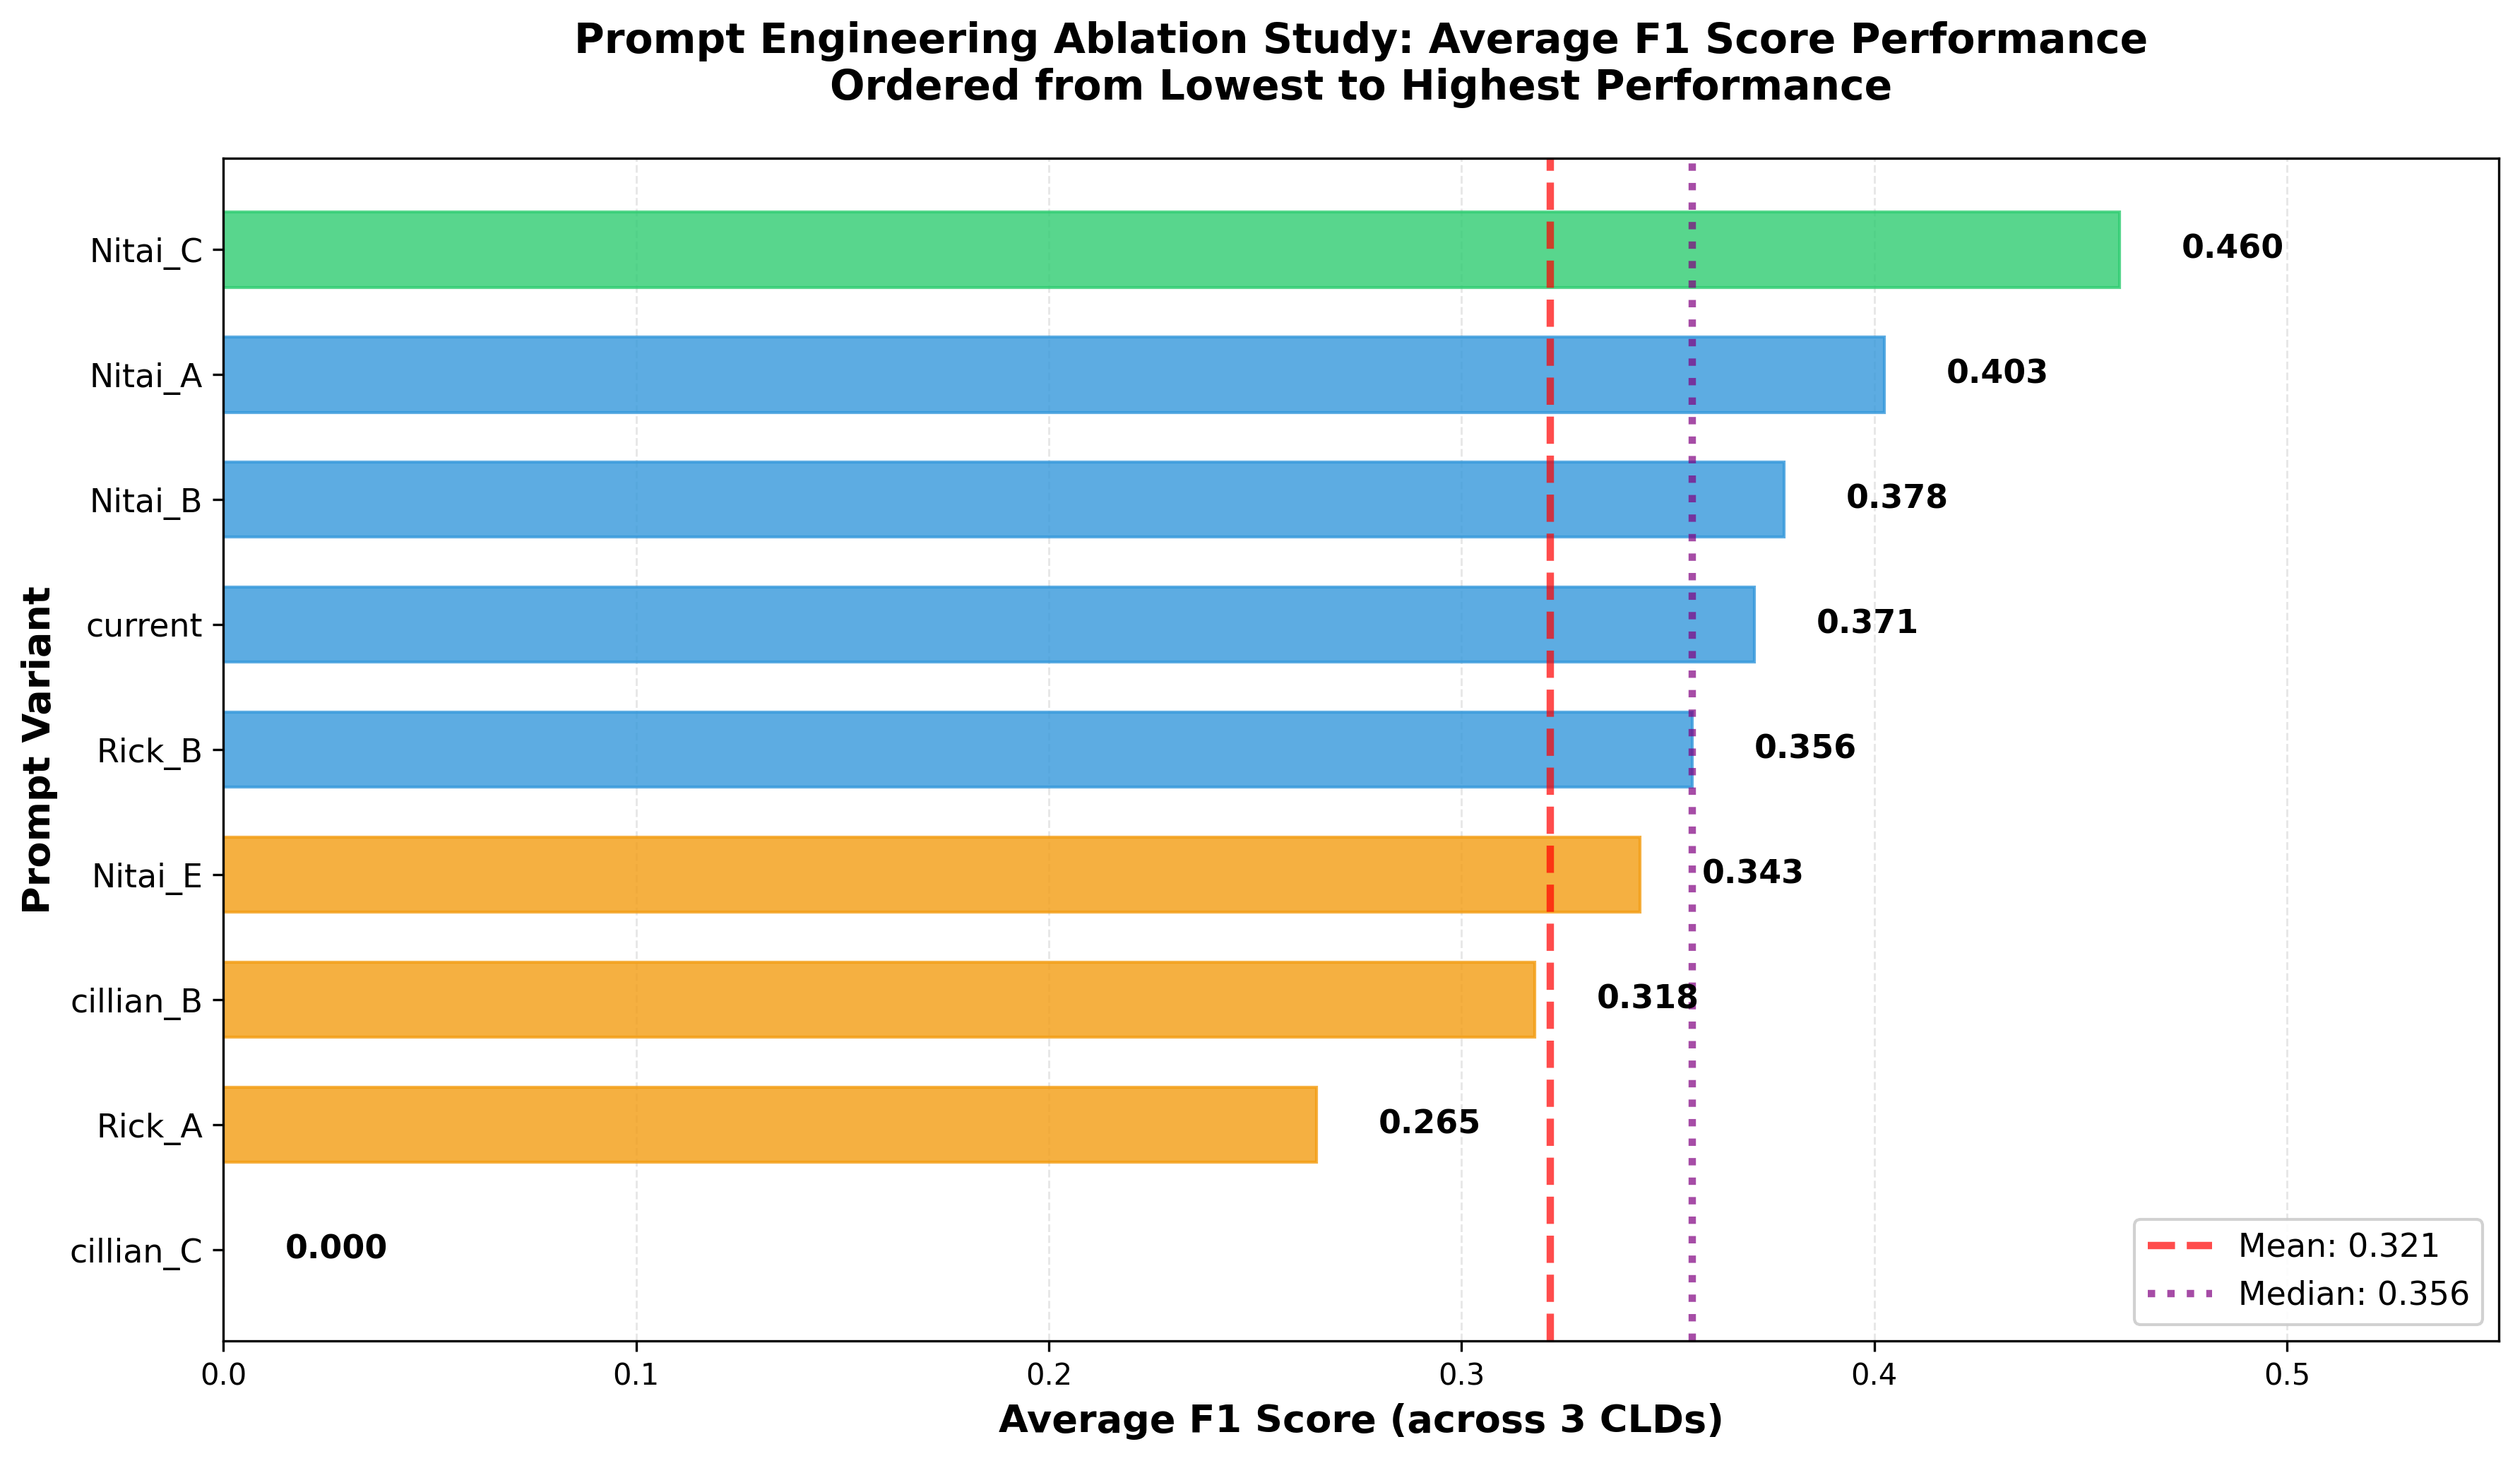
\includegraphics[width=0.95\textwidth]{../Figures/edge_ablation_f1_ordered.png}
    \caption[Average F1 by prompt]{Average F1 scores for prompt variants across three CLDs, ordered from lowest to highest. Nitai\_C achieved highest performance (F1=0.460). Colour coding: green (F1 $\geq$ 0.45), blue (0.35--0.45), orange (0.25--0.35), red ($<$0.25).}
    \label{fig:ablation_f1_ordered}
\end{figure}

\begin{table}[H]
\centering
\caption{F1 Scores by Prompt Variant and Causal Loop Diagram}
\label{tab:f1_scores}
\begin{tabular}{@{}lcccc@{}}
\toprule
\textbf{Prompt} & \textbf{CLD 1} & \textbf{CLD 2} & \textbf{CLD 3} & \textbf{Average} \\
\midrule
Nitai\_C & 0.591 & 0.204 & 0.583 & \textbf{0.460} \\
Nitai\_A & 0.590 & 0.218 & 0.400 & 0.403 \\
Nitai\_B & 0.588 & 0.092 & 0.455 & 0.378 \\
Current & 0.588 & 0.239 & 0.286 & 0.371 \\
Rick\_B & 0.444 & 0.186 & 0.438 & 0.356 \\
Nitai\_E & 0.438 & 0.207 & 0.385 & 0.343 \\
Cillian\_B & 0.515 & 0.152 & 0.286 & 0.318 \\
Rick\_A & 0.380 & 0.145 & 0.269 & 0.265 \\
Cillian\_C & 0.000 & 0.000 & 0.000 & 0.000 \\
\bottomrule
\end{tabular}
\end{table}

\subsection{Key Findings}

\textbf{Overall Performance:}
\begin{itemize}[noitemsep]
    \item \textbf{Best Performance}: Nitai\_C achieved the highest average F1 score (0.460), differing from others in multiple dimensions (dual-level CoT, relationship taxonomy, examples).
    \item \textbf{Performance Range}: Range of 0.195 between best (0.460) and second-worst (0.265) performers. Mean F1 = 0.321, SD = 0.132.
\end{itemize}

\textbf{CLD-Specific Patterns:}
\begin{itemize}[noitemsep]
    \item \textbf{CLD 2 Challenge}: All variants performed worst on CLD 2 (Social Norms), with F1 scores 0.00--0.24.
    \item \textbf{High Variance}: Within-prompt SD across CLDs ranged 0.18--0.25, indicating sensitivity to problem characteristics.
\end{itemize}

\textbf{Technique-Specific Observations:}
\begin{itemize}[noitemsep]
    \item \textbf{RAG Trade-off}: Nitai\_E (mandatory citations) showed 25\% lower performance than Nitai\_C, suggesting strict citation requirements limit valid relationship discovery.
    \item \textbf{Complete Failure}: Cillian\_C's zero performance indicates overly restrictive definition-grounded evaluation can be counterproductive.
\end{itemize}

\subsection{Interpretation}

The progression Nitai\_A $\rightarrow$ Nitai\_B $\rightarrow$ Nitai\_C demonstrates incremental performance gains with Chain-of-Thought, achieving 14\% improvement over baseline. This supports Wei et al.'s~\cite{wei2022chain} findings that explicit reasoning steps enhance complex task performance.

Rick\_B (F1=0.356), employing systematic decomposition, underperformed Nitai\_C's CoT approach by 23\%, suggesting decomposition strategies may be less effective when tasks require holistic pattern recognition rather than sequential problem solving.

\subsection{Limitations}

\begin{itemize}[noitemsep]
    \item \textbf{Sample Size}: Only three CLDs limits generalizability.
    \item \textbf{Single Run}: Each variant tested once per CLD, preventing statistical significance testing.
    \item \textbf{Model Specificity}: Results apply to GPT-4.1; patterns may differ for other LLMs.
    \item \textbf{Prompt Authorship}: Different variants designed by different researchers, introducing potential confounding.
\end{itemize}

\section{Generator Design Rationale}
\label{app:generator_design_rationale}
% ------------------------------------------------------------------------------

This section motivates the generator's decomposition into edge-level decisions and the accompanying safeguards used in our experiments.

In our CLD generation system, given temporal and spatial scales and domain context, we generate a set of nodes (or, in the main experiments, insert validated nodes by fixing the node set to the ground-truth validation variables \(V\)), and then generate relationships pairwise as directed queries over ordered variable pairs \((A,B)\) and \((B,A)\) (i.e., \( |V|(|V|-1)\) candidate edges). For each directed pair, the LLM is asked whether \(A\) \emph{directly} causes \(B\) and to return a relationship type and a short causal narrative; in this study, relationship types are constrained to \{\texttt{POSITIVE}, \texttt{NEGATIVE}, \texttt{NONE}\} (Section~\ref{sec:generator_prompt_nitai_c}, Listing~\ref{lst:generator_nitai_c_yaml}). To address the limitation of reviewing links in isolation, we perform a mediation check by passing the current node set \(V\) to the edge prompt as candidate mediators. When supported by the LLM API, we also capture token-level logprobs for the edge-generation response (relationship label + narrative) and derive logprob-based uncertainty features (LUQ metrics) used in downstream hallucination detection. Algorithmic details are traced from the implementation in Section~\ref{sec:algorithms} (Algorithm~\ref{alg:cld_generation}). Relative to Crielaard et al.'s CLD-to-SDM pipeline (Section~\ref{sec:background_gmb}; \citet{crielaard2024refining}), this operationalises the \emph{causal link identification} step and approximates \emph{intermediary-variable documentation} via mediation checks over the current node set, while deferring richer aCLD elements such as functional forms and interaction terms to future work (i.e., these are not addressed in this thesis). Our downstream phases address evidence-quality annotation through post-hoc edge validation and remediation (LLM-as-a-Judge and LLM-as-a-Corrector) and, when allocating additional test-time compute, external evidence acquisition via Deep Research (RQ3).

\section{Generator Prompt (Nitai\_C)}
\label{sec:generator_prompt_nitai_c}
% ------------------------------------------------------------------------------

The final experiments use the \textbf{Nitai\_C} generator prompt configuration for both node generation (\texttt{generateNodes}) and edge generation (\texttt{generateEdges}). The prompt is stored at:

\noindent\texttt{data\_science/parameter\_tuning\_experiments/prompts\_Nitai\_C.yaml}

\noindent and is archived (as a copied file) at:

\noindent\texttt{final\_runs/prompts/PRELIM\_generator/final\_generator/prompts\_Nitai\_C.yaml}

\noindent (see \texttt{final\_runs/prompts/README.md} for IDs and checksums).

\begin{lstlisting}[caption={Generator Prompt Configuration: Nitai\_C (\texttt{generateNodes} + \texttt{generateEdges})},label={lst:generator_nitai_c_yaml}]
PROMPT ARCHIVE NOTE:
- Full prompt text is archived as a copied YAML at:
  final_runs/prompts/PRELIM_generator/final_generator/prompts_Nitai_C.yaml
- See: final_runs/prompts/README.md
\end{lstlisting}

Three prompting strategies were evaluated for each component:
\begin{enumerate}[noitemsep]
    \item \textbf{Baseline}: Direct instruction without reasoning scaffolding (control condition)
    \item \textbf{Chain-of-Thought (CoT)}: Zero-shot CoT via ``Let's think step by step''~\citep{kojima2022large}
    \item \textbf{Mechanistic}: Domain-specific criteria based on the Bradford Hill causal framework~\citep{shimonovich2020bradford}
\end{enumerate}

For citation judges, an additional \textbf{Mechanistic-Lit} variant combines mechanistic evaluation with explicit literature grounding requirements.

% ------------------------------------------------------------------------------
\section{Edge Generation Ablation Prompts}
\label{sec:edge_ablation_prompts}
% ------------------------------------------------------------------------------

The full text of all nine edge-generation prompt variants used in the ablation study (Section~\ref{sec:ablation_edge}) is archived (as copies) under:

\noindent\texttt{final\_runs/prompts/PRELIM\_generator/edge\_ablation/}

\noindent See \texttt{final\_runs/prompts/README.md} for stable IDs and file checksums.

\noindent (Prompts are not reproduced verbatim here to minimize appendix length.)

\chapter{Node Generation Prompt Ablation}
\label{sec:ablation_node}

Seven prompt variants were evaluated in a full factorial design: 7 prompts $\times$ 3 CLDs $\times$ 5 runs = 105 total experiments.

\begin{table}[H]
\centering
\caption{Node Generation Ablation: Hybrid F1 Scores by Prompt Variant}
\label{tab:node_ablation}
\footnotesize
\begin{tabular}{@{}lccccc@{}}
\toprule
\textbf{Prompt} & \textbf{Mean F1} & \textbf{Std} & \textbf{95\% CI} & \textbf{Cohen's $d$ (vs.\ baseline)} & \textbf{N} \\
\midrule
Node\_V6\_Andrew & 0.677 & 0.079 & [0.638, 0.717] & +0.44 & 15 \\
Node\_V3\_CoT\_System & 0.657 & 0.123 & [0.595, 0.719] & +0.16 & 15 \\
Node\_V0\_Minimal (baseline) & 0.639 & 0.094 & [0.592, 0.687] & --- & 15 \\
Node\_V5\_Nitai\_C & 0.636 & 0.088 & [0.591, 0.680] & -0.04 & 15 \\
Node\_V1\_Role\_Only & 0.628 & 0.080 & [0.588, 0.669] & -0.13 & 15 \\
Node\_V4\_CoT\_User & 0.619 & 0.104 & [0.567, 0.672] & -0.20 & 15 \\
Node\_V2\_Constraints & 0.617 & 0.077 & [0.578, 0.656] & -0.26 & 15 \\
\bottomrule
\end{tabular}
\end{table}

\textbf{Statistical Analysis:}
\begin{itemize}[noitemsep]
    \IfFileExists{generated/node_ablation_stats.tex}{
        % Node ablation statistics - auto-generated placeholder
\item Node ablation analysis: No significant differences detected

    }{
        \item One-way ANOVA: $F = 0.81$, $p = 0.567$ --- \textbf{no significant differences}
        \item All pairwise comparisons non-significant after Bonferroni correction
        \item Effect sizes negligible to small (Cohen's $d$ vs.\ baseline range: $-0.26$ to $+0.44$)
    }
\end{itemize}

\textbf{Interpretation:} Unlike edge generation, node generation is robust to prompt engineering variations. The minimal baseline performed comparably to sophisticated Chain-of-Thought variants, suggesting that node identification is a simpler task for LLMs that does not benefit substantially from advanced prompting strategies.

\section{Node Generation Prompts}
\label{sec:node_prompts}

The full text of all seven node-generation prompt variants used in the node ablation study (Section~\ref{sec:ablation_node}) is archived (as copies) under:

\noindent\texttt{final\_runs/prompts/PRELIM\_generator/node\_ablation/}

\noindent See \texttt{final\_runs/prompts/README.md} for stable IDs and file checksums.

\noindent (Prompts are not reproduced verbatim here to minimize appendix length.)

\chapter{Embedding Model Benchmark}
\label{sec:embedding_benchmark}

To justify the choice of embedding model for cosine similarity computation (Section~2.5), we benchmarked \texttt{all-mpnet-base-v2} against the MTEB-leading Qwen3-Embedding-8B using 30 real causal narratives from our CLD experiments.

\begin{table}[H]
\centering
\caption{Embedding Model Benchmark ($n=30$ causal narratives from CLD)}
\label{tab:embed_benchmark}
\footnotesize
\begin{tabular}{@{}lcccc@{}}
\toprule
\textbf{Model} & \textbf{Params} & \textbf{Embed dim} & \textbf{ms/doc} & \textbf{docs/s} \\
\midrule
all-mpnet-base-v2 & 110M & 768 & 3.0 & 336 \\
Qwen3-Embedding-8B (Q4) & 8B & 4096 & 67.3 & 14.9 \\
\bottomrule
\end{tabular}
\end{table}

\textbf{Compute setup:} Hardware details are reported in Appendix~\ref{sec:software_env} (Table~\ref{tab:system_env}). Qwen3 was run via Ollama with 4-bit quantization (Q4\_K\_M).

\textbf{Test data:} Causal narratives averaged 451 characters ($\sim$100 tokens). In production, fetched citation documents are chunked up to 4,000 characters ($\sim$1,000 tokens) before embedding---longer inputs may increase per-document latency.

\textbf{MTEB Benchmark Comparison:}

\begin{table}[H]
\centering
\caption{MTEB Scores: MPNet vs.\ Qwen3-Embedding-8B}
\label{tab:mteb_comparison}
\footnotesize
\begin{tabular}{@{}lcc@{}}
\toprule
\textbf{Task} & \textbf{MPNet (110M)\textsuperscript{a}} & \textbf{Qwen3-8B\textsuperscript{b}} \\
\midrule
STS (Spearman $\rho$) & 80.28 & \textbf{88.58} \\
Reranking (MAP) & \textbf{59.36} & 51.56 \\
Pair Classification (AP) & 83.04 & \textbf{87.52} \\
Classification (Acc) & 65.07 & \textbf{90.43} \\
Clustering (V-measure) & 43.69 & \textbf{58.57} \\
Retrieval (nDCG@10) & 43.81 & \textbf{69.44} \\
Summarization & 27.49 & \textbf{34.83} \\
\midrule
\textbf{Average} & 57.78 & \textbf{75.22} \\
\bottomrule
\end{tabular}

\vspace{0.3em}
\raggedright\scriptsize
\textsuperscript{a}Muennighoff et al.~\cite{muennighoff2023mteb}, Table 1 (MTEB v1, 2022). \textsuperscript{b}Zhang et al.~\cite{qwen3embedding2025}, Table 7 (MTEB eng v2, 2025).
\end{table}

\textbf{Result:} MPNet achieves 22$\times$ faster inference (3.0 vs.\ 67.3~ms/doc; Table~\ref{tab:embed_benchmark}). Since cosine-similarity scoring is used as a throughput-bound heuristic for max-similarity chunk selection, we prioritise latency; MPNet is a strong general-purpose embedding model and is widely used in practice.

\textit{Note:} The MTEB scores are taken from different benchmark versions (v1 vs.\ v2) and evaluation setups and are therefore \textbf{not directly comparable}. We include them only to illustrate that both models are competitive across common embedding tasks.

\textbf{Script:} \texttt{final\_runs/supp\_embedding\_benchmark/embedding\_benchmark\_real\_cld.py}

%==============================================================================
\chapter{Algorithmic Descriptions}
\label{sec:algorithms}
%==============================================================================

This section provides formal algorithmic descriptions of the core system components, traced directly from the implementation. For experimental design rationale, see the corresponding Methods sections.

\section{Algorithm 0: CLD Generation}
\label{alg:cld_generation}

The CLD generator constructs causal loop diagrams through a two-phase process: node generation followed by edge generation. Both phases capture UQ metrics via logprobs for downstream hallucination detection.

\begin{table}[H]
\centering
\caption{CLD Generation (\texttt{generate\_variables} + \texttt{discover\_relationships})}
\footnotesize
\begin{tabular}{@{}r l@{}}
\toprule
\multicolumn{2}{@{}l}{\textbf{Input:} target\_variable, temporal\_scale, spatial\_scale, num\_variables, context} \\
\multicolumn{2}{@{}l}{\textbf{Output:} Neo4j session with nodes (variables) and edges (relationships) + UQ metrics} \\
\midrule
\multicolumn{2}{@{}l}{\textit{// Phase 1: Node Generation (generateNodes prompt)}} \\
1. & session\_id $\leftarrow$ uuid.generate() \\
2. & Neo4j.create\_node(target\_variable, is\_target=True, session\_id) \\
3. & variables $\leftarrow$ [target\_variable] \\
4. & \textbf{while} len(variables) $<$ num\_variables: \\
5. & \quad vars $\leftarrow$ \{target, target\_units, target\_definition, temporal, spatial, context\} \\
6. & \quad (sys\_prompt, usr\_prompt) $\leftarrow$ tree.build\_prompt(``generateNodes'', vars) \\
7. & \quad usr\_prompt $\leftarrow$ usr\_prompt + ``Exclude: '' + join(variables) \\
8. & \quad response $\leftarrow$ generator\_llm.send\_message(prompts, logprobs=True, top\_logprobs=5) \\
9. & \quad (name, definition, units, citations) $\leftarrow$ tree.read\_variable\_response(response) \\
10. & \quad log\_metrics $\leftarrow$ compute\_uq\_metrics(response.logprobs) \\
11. & \quad Neo4j.create\_node(name, definition, citations, log\_metrics, session\_id) \\
12. & \quad variables.append(name) \\
\midrule
\multicolumn{2}{@{}l}{\textit{// Phase 2: Edge Generation (generateEdges prompt)}} \\
13. & pairs $\leftarrow$ generate\_ordered\_pairs(variables) \hfill\textit{// $N^2$ pairs, excludes self-loops} \\
14. & \textbf{for each} (source, target) $\in$ pairs: \\
15. & \quad (source\_def, target\_def) $\leftarrow$ Neo4j.fetch\_definitions(source, target) \\
16. & \quad vars $\leftarrow$ \{var1: source, var2: target, def1, def2, temporal, spatial, variables\} \\
17. & \quad (sys\_prompt, usr\_prompt) $\leftarrow$ tree.build\_prompt(``generateEdges'', vars) \\
18. & \quad response $\leftarrow$ generator\_llm.send\_message(prompts, logprobs=True, top\_logprobs=5) \\
19. & \quad (rel\_type, motivation, citations) $\leftarrow$ tree.read\_relationships(response) \\
20. & \quad log\_metrics $\leftarrow$ compute\_ci\_metrics(response.logprobs) \\
21. & \quad Neo4j.create\_relationship(source, target, rel\_type, motivation, citations, log\_metrics) \\
22. & \textbf{return} session\_id, variables, relationships \\
\bottomrule
\end{tabular}
\end{table}

\noindent\textbf{Implementation:} \texttt{modules.py:698} (\texttt{generate\_variables}), \texttt{:1147} (\texttt{discover\_relationships}),\\ \texttt{:908} (\texttt{process\_variable\_pair})

\noindent\textbf{Acknowledgement:} The CLD generation algorithm was conceived by Rick Quax with feedback from Cillian Hourican and implemented by Andrew Crossley. The author (Nitai Nijholt) contributed the mediation check, multi-provider LLM infrastructure with rate limiting and fallbacks, and prompt testing framework.

\section{Algorithm 1: Judge-Correctness}
\label{alg:judge_correctness}

The correctness-based judge evaluates causal reasoning quality without external evidence.

\begin{table}[H]
\centering
\caption{Judge-Correctness (\texttt{judge\_all\_edges\_serial}, approach=``correctness'')}
\footnotesize
\begin{tabular}{@{}r l@{}}
\toprule
\multicolumn{2}{@{}l}{\textbf{Input:} session\_id, judge\_models[], prompt\_config} \\
\multicolumn{2}{@{}l}{\textbf{Output:} Per-edge verdicts with scores} \\
\midrule
1. & edges $\leftarrow$ Neo4j.query(``MATCH (s)-[r]->(t) WHERE s.session\_id = \$sid'') \\
2. & judges[] $\leftarrow$ create\_llm\_clients(judge\_models) \\
3. & \textbf{for each} edge $\in$ edges: \\
4. & \quad text $\leftarrow$ edge.spurious\_motivation $\lor$ edge.motivation \\
5. & \quad \textbf{if} text = $\emptyset$: verdict $\leftarrow$ ``NO\_MOTIVATION''; \textbf{continue} \\
6. & \quad variables $\leftarrow$ \{source, target, relationship, motivation: text\} \\
7. & \quad (sys\_prompt, usr\_prompt) $\leftarrow$ tree.build\_prompt(``judgeCorrectness'', vars) \\
8. & \quad scores[], verdicts[] $\leftarrow$ [], [] \\
9. & \quad \textbf{for each} judge $\in$ judges: \\
10. & \quad\quad response $\leftarrow$ judge.send\_message(sys\_prompt, usr\_prompt, logprobs=True) \\
11. & \quad\quad (verdict, score, reason) $\leftarrow$ parse\_regex(response, ``VERDICT: SCORE:'') \\
12. & \quad\quad verdicts.append(verdict); scores.append(score) \\
13. & \quad aggregate\_score $\leftarrow$ mean(scores) \\
14. & \quad aggregate\_verdict $\leftarrow$ majority\_vote(verdicts) \\
15. & \quad update\_edge(edge, aggregate\_verdict, aggregate\_score) \\
16. & \textbf{return} judged\_edges \\
\bottomrule
\end{tabular}
\end{table}

\textbf{Implementation:} \texttt{modules.py:4421} $\rightarrow$ \texttt{:4740} (correctness branch)

\section{Algorithm 2: Judge-Citation}
\label{alg:judge_citation}

The citation-based judge validates causal claims against fetched scientific literature.

\begin{table}[H]
\centering
\caption{Judge-Citation (\texttt{judge\_all\_edges\_with\_citations\_serial})}
\footnotesize
\begin{tabular}{@{}r l@{}}
\toprule
\multicolumn{2}{@{}l}{\textbf{Input:} session\_id, judge\_models[], citation\_fetcher} \\
\multicolumn{2}{@{}l}{\textbf{Output:} Per-edge aggregate verdicts with per-citation scores} \\
\midrule
1. & edges $\leftarrow$ Neo4j.query(``MATCH (s)-[r]->(t) WHERE s.session\_id = \$sid'') \\
2. & judges[] $\leftarrow$ create\_llm\_clients(judge\_models) \\
3. & \textbf{for each} edge $\in$ edges: \\
4. & \quad citations $\leftarrow$ edge.citations \\
5. & \quad \textbf{if} citations = $\emptyset$: verdict $\leftarrow$ ``NO\_CITATION''; \textbf{continue} \\
6. & \quad citation\_contents $\leftarrow$ ContentScraper.process\_citations(citations) \\
7. & \quad per\_citation\_results $\leftarrow$ [] \\
8. & \quad \textbf{for each} (url, content) $\in$ citation\_contents: \\
9. & \quad\quad prompt $\leftarrow$ build\_citation\_prompt(edge.motivation, content) \\
10. & \quad\quad judge\_verdicts $\leftarrow$ [] \\
11. & \quad\quad \textbf{for each} judge $\in$ judges: \\
12. & \quad\quad\quad response $\leftarrow$ judge.send\_message(prompt) \\
13. & \quad\quad\quad verdict $\leftarrow$ parse(response) \hfill\textit{// SUPPORTED/PARTIAL/CONTRADICTED} \\
14. & \quad\quad\quad judge\_verdicts.append(verdict) \\
15. & \quad\quad citation\_verdict $\leftarrow$ majority\_vote(judge\_verdicts) \\
16. & \quad\quad citation\_score $\leftarrow$ verdict\_to\_score(citation\_verdict) \hfill\textit{// 1.0, 0.5, 0.0} \\
17. & \quad\quad per\_citation\_results.append(\{url, citation\_verdict, citation\_score\}) \\
18. & \quad aggregate\_score $\leftarrow$ mean(per\_citation\_results.scores) \\
19. & \quad aggregate\_verdict $\leftarrow$ aggregator\_llm(per\_citation\_results) \\
20. & \quad update\_edge(edge, aggregate\_verdict, aggregate\_score) \\
21. & \textbf{return} judged\_edges \\
\bottomrule
\end{tabular}
\end{table}

\textbf{Implementation:} \texttt{modules.py:5688} (\texttt{judge\_all\_edges\_with\_citations\_serial}) $\rightarrow$ \texttt{modules.py:4988}

\section{Algorithm 3: Corruption}
\label{alg:corruption}

The corruptor introduces controlled errors using stratified sampling for balanced corruption types.

\noindent\textbf{Parameters used in this thesis (GT Synth).} Unless otherwise stated, corruption experiments use \texttt{corruption\_rate=0.3} with a balanced 1/3 split across corruption types (motivation corruption, spurious edges, polarity flips). The corruptor LLM configuration is \texttt{model=gpt-4.1}, \texttt{temperature=0.7}, \texttt{top\_p=1.0}; corruption is seeded for reproducibility (see \texttt{corruption\_metadata.json} in the corresponding \texttt{final\_runs/} output directory).

\begin{table}[H]
\centering
\caption{Corruption (\texttt{\_corrupt\_relationships})}
\footnotesize
\begin{tabular}{@{}r l@{}}
\toprule
\multicolumn{2}{@{}l}{\textbf{Input:} session\_id, corruption\_rate (default 0.3), seed, corruptor\_llm} \\
\multicolumn{2}{@{}l}{\textbf{Output:} Number of corrupted edges, corruption metadata} \\
\midrule
1. & random.seed(seed) \hfill\textit{// Reproducibility} \\
2. & edges $\leftarrow$ Neo4j.query(``MATCH (s)-[r]->(t)'') \\
3. & none\_edges $\leftarrow$ \{e $\in$ edges : e.type = ``NONE''\} \\
4. & causal\_edges $\leftarrow$ \{e $\in$ edges : e.type $\in$ \{``POSITIVE'', ``NEGATIVE''\}\} \\
5. & n\_corrupt $\leftarrow$ $\lfloor$len(edges) $\times$ corruption\_rate$\rfloor$ \\
6. & target\_per\_type $\leftarrow$ n\_corrupt $\div$ 3 \hfill\textit{// Balanced: 1/3 each} \\
7. & spurious\_sample $\leftarrow$ shuffle(none\_edges)[:target\_per\_type] \\
8. & causal\_sample $\leftarrow$ shuffle(causal\_edges)[:target\_per\_type $\times$ 2] \\
9. & \textbf{for each} edge $\in$ spurious\_sample $\cup$ causal\_sample: \\
10. & \quad \textbf{if} edge.type = ``NONE'': corruption\_type $\leftarrow$ ``spurious\_edge'' \\
11. & \quad \textbf{else}: corruption\_type $\leftarrow$ argmin(assigned[``polarity\_flip''], assigned[``motivation'']) \\
12. & \quad assigned[corruption\_type] += 1 \\
13. & \quad \textbf{if} corruption\_type = ``motivation'': \\
14. & \quad\quad prompt $\leftarrow$ tree.build\_prompt(``corruptor'', edge) \\
15. & \quad\quad edge.spurious\_motivation $\leftarrow$ corruptor\_llm.send(prompt) \\
16. & \quad \textbf{elif} corruption\_type = ``spurious\_edge'': \\
17. & \quad\quad prompt $\leftarrow$ tree.build\_prompt(``generateSpuriousEdge'', edge) \\
18. & \quad\quad \{type, expl\} $\leftarrow$ JSON.parse(corruptor\_llm.send(prompt)) \\
19. & \quad\quad Neo4j: DELETE NONE, CREATE edge.type $\leftarrow$ type, motivation $\leftarrow$ expl \\
20. & \quad \textbf{elif} corruption\_type = ``polarity\_flip'': \\
21. & \quad\quad prompt $\leftarrow$ tree.build\_prompt(``generateFlippedPolarity'', edge) \\
22. & \quad\quad \{expl\} $\leftarrow$ JSON.parse(corruptor\_llm.send(prompt)) \\
23. & \quad\quad Neo4j: DELETE old, CREATE edge.type $\leftarrow$ flip(type), motivation $\leftarrow$ expl \\
24. & \quad edge.is\_corrupted $\leftarrow$ True \\
25. & save\_metadata(``corrupted\_relationships\_\{session\_id\}.json'') \\
26. & \textbf{return} corrupted\_count \\
\bottomrule
\end{tabular}
\end{table}

\textbf{Implementation:} \texttt{modules.py:1748} (\texttt{\_corrupt\_relationships}), \texttt{:1544} (\texttt{\_corrupt\_relationship}), \texttt{:1582} (\texttt{\_convert\_none\_to\_spurious}), \texttt{:1645} (\texttt{\_flip\_edge\_polarity})

\section{Algorithm 4: Corrector}
\label{alg:corrector}

The corrector applies LLM-guided fixes to edges flagged by the judge.

\begin{table}[H]
\centering
\caption{Corrector (\texttt{correct\_edges\_serial})}
\footnotesize
\begin{tabular}{@{}r l@{}}
\toprule
\multicolumn{2}{@{}l}{\textbf{Input:} session\_id, corrector\_models[], action\_order, rejudge\_after} \\
\multicolumn{2}{@{}l}{\textbf{Output:} Correction outcomes per edge} \\
\midrule
1. & candidates $\leftarrow$ Neo4j.query(``WHERE r.verdict IN [`INCORRECT', `PARTIAL', ...]'') \\
2. & agent $\leftarrow$ create\_corrector\_agent(corrector\_models[0], prompt\_variant) \\
3. & available\_vars $\leftarrow$ get\_all\_variables(session\_id) \\
4. & outcomes $\leftarrow$ [] \\
5. & \textbf{for each} edge $\in$ candidates: \\
6. & \quad context $\leftarrow$ \{edge, available\_vars, graph\_structure\} \\
7. & \quad \textbf{for each} action $\in$ action\_order: \hfill\textit{// revise\_motivation, change\_edge\_type} \\
8. & \quad\quad result $\leftarrow$ agent.call\_tool(action, edge, context) \\
9. & \quad\quad \textbf{if} result.success: \\
10. & \quad\quad\quad outcomes.append(\{edge, action, corrected: True\}); \textbf{break} \\
11. & \textbf{if} rejudge\_after: \\
12. & \quad judge\_all\_edges\_with\_citations\_serial(approach=rejudge\_approach) \\
13. & \textbf{return} outcomes \\
\bottomrule
\end{tabular}
\end{table}

\textbf{Implementation:} \texttt{modules.py:7050} (\texttt{correct\_edges\_serial})

\section{Algorithm 5: UQ Metrics Computation}
\label{alg:uq_metrics}

Uncertainty Quantification (UQ) metrics computed from LLM logprobs during generation.

\begin{table}[H]
\centering
\caption{UQ Metrics (\texttt{logit\_metrics.py})}
\footnotesize
\begin{tabular}{@{}r l@{}}
\toprule
\multicolumn{2}{@{}l}{\textbf{Input:} logprobs = \{tokens[], token\_logprobs[], top\_logprobs[]\}} \\
\multicolumn{2}{@{}l}{\textbf{Output:} perplexity, min\_prob, max\_window\_entropy, cosine\_sim} \\
\midrule
\multicolumn{2}{@{}l}{\textit{// Perplexity (compute\_avg\_nll + exp)}} \\
1. & nll\_capped $\leftarrow$ [$\min$(-logprob$_i$, 20.0) for logprob$_i$ in token\_logprobs] \\
2. & avg\_nll $\leftarrow$ mean(nll\_capped) \\
3. & avg\_nll\_capped $\leftarrow$ $\min$(avg\_nll, 10.0) \\
4. & perplexity $\leftarrow$ $\exp$(avg\_nll\_capped) \\
\multicolumn{2}{@{}l}{\textit{// Minimum Token Probability (compute\_min\_prob)}} \\
5. & probs $\leftarrow$ [$\exp$(logprob$_i$) for logprob$_i$ in token\_logprobs] \\
6. & min\_prob $\leftarrow$ $\min$(probs) \\
\multicolumn{2}{@{}l}{\textit{// Max Window Entropy (compute\_max\_window\_entropy)}} \\
7. & entropies $\leftarrow$ [] \\
8. & \textbf{for each} top\_k\_dict $\in$ top\_logprobs: \\
9. & \quad p\_vals $\leftarrow$ softmax(top\_k\_dict.values()) \\
10. & \quad H $\leftarrow$ $-\sum_i$ p$_i$ $\log$(p$_i$) \\
11. & \quad entropies.append(H) \\
12. & windowed $\leftarrow$ convolve(entropies, window\_size=5) \\
13. & max\_window\_entropy $\leftarrow$ $\max$(windowed) \\
\multicolumn{2}{@{}l}{\textit{// Cosine Similarity (get\_embedding\_local)}} \\
14. & e$_{\text{narr}}$ $\leftarrow$ SentenceTransformer(motivation, model=``all-mpnet-base-v2'') \\
15. & e$_{\text{cit}}$ $\leftarrow$ SentenceTransformer(citation\_text) \\
16. & cosine\_sim $\leftarrow$ $\max_c$ $\frac{\mathbf{e}_{\text{narr}} \cdot \mathbf{e}_c}{\|\mathbf{e}_{\text{narr}}\| \|\mathbf{e}_c\|}$ \\
17. & \textbf{return} \{perplexity, min\_prob, max\_window\_entropy, cosine\_sim\} \\
\bottomrule
\end{tabular}
\end{table}

\textbf{Implementation:} \texttt{logit\_metrics.py} -- \texttt{:177} (avg\_nll), \texttt{:251} (min\_prob), \texttt{:259} (max\_entropy), \texttt{:98} (embedding)

\section{Algorithm 6: Hallucination Classification}
\label{alg:classification}

Ensemble classifiers trained on UQ metrics to predict hallucinations.

\begin{table}[H]
\centering
\caption{Hallucination Classification (\texttt{train\_classifiers})}
\footnotesize
\begin{tabular}{@{}r l@{}}
\toprule
\multicolumn{2}{@{}l}{\textbf{Input:} X = [perplexity, min\_prob, max\_entropy, cosine\_sim], y = hallucination\_labels} \\
\multicolumn{2}{@{}l}{\textbf{Output:} Trained models, metrics (AUC, Precision, Recall, F1)} \\
\midrule
1. & X\_scaled $\leftarrow$ StandardScaler.fit\_transform(X) \\
2. & (X\_train, X\_test, y\_train, y\_test) $\leftarrow$ train\_test\_split(X\_scaled, y, test=0.3) \\
3. & classifiers $\leftarrow$ \{LogReg, RandomForest(100), GradBoost(100), MLP(32,16)\} \\
4. & \textbf{for each} (name, clf) $\in$ classifiers: \\
5. & \quad cv $\leftarrow$ StratifiedKFold(n\_splits=5) \\
6. & \quad cv\_auc $\leftarrow$ cross\_val\_score(clf, X\_train, y\_train, cv, scoring=``roc\_auc'') \\
7. & \quad clf.fit(X\_train, y\_train) \\
8. & \quad y\_pred\_proba $\leftarrow$ clf.predict\_proba(X\_test)[:,1] \\
9. & \quad metrics[name].auc $\leftarrow$ roc\_auc\_score(y\_test, y\_pred\_proba) \\
10. & \quad metrics[name].\{precision, recall, f1\} $\leftarrow$ precision\_recall\_fscore(y\_test, y\_pred) \\
11. & \textbf{return} classifiers, metrics \\
\bottomrule
\end{tabular}
\end{table}

\textbf{Implementation:} \texttt{rq2\_ensemble\_classifier.py:32} (\texttt{train\_classifiers})

\section{Algorithm 7: Citation Search (Brave)}
\label{alg:citation_search_brave}

This procedure retrieves candidate citation URLs for a CLD edge using the Brave Search API, optionally filtered by a trusted-domain whitelist (\cite{bravesearchapi}). It is invoked during citation filling when no usable citations are available from the LLM, and can also be used to obtain candidate sources for citation-based judging.

\vspace{0.25em}
\noindent\textbf{Trusted Academic Domains (23):} Results from the following domains are prioritised (\cite{bravesearchapi}):
\begin{itemize}[noitemsep]
    \item \texttt{pubmed.ncbi.nlm.nih.gov}
    \item \texttt{arxiv.org}
    \item \texttt{scholar.google.com}
    \item \texttt{nature.com}
    \item \texttt{science.org}
    \item \texttt{cell.com}
    \item \texttt{nejm.org}
    \item \texttt{bmj.com}
    \item \texttt{plos.org}
    \item \texttt{frontiersin.org}
    \item \texttt{springer.com}
    \item \texttt{wiley.com}
    \item \texttt{sciencedirect.com}
    \item \texttt{tandfonline.com}
    \item \texttt{sage.com}
    \item \texttt{jstor.org}
    \item \texttt{cochranelibrary.com}
    \item \texttt{nih.gov}
    \item \texttt{who.int}
    \item \texttt{cdc.gov}
    \item \texttt{academic.oup.com}
    \item \texttt{cambridge.org}
    \item \texttt{elsevier.com}
\end{itemize}

\begin{table}[H]
\centering
\caption{Citation Search (\texttt{\_search\_with\_brave} + \texttt{SearchEngine.search})}
\footnotesize
\begin{tabular}{@{}r l@{}}
\toprule
\multicolumn{2}{@{}l}{\textbf{Input:} src, rel, tgt, claim\_txt, api\_key, trusted\_domains[] (optional)} \\
\multicolumn{2}{@{}l}{\textbf{Output:} citations[] (URLs, up to 5)} \\
\midrule
\multicolumn{2}{@{}l}{\textit{// Phase 0: Initialize Brave client (once per run)}} \\
1. & search\_client $\leftarrow$ SearchEngine(api\_key, trusted\_domains) \\
2. & session $\leftarrow$ requests.Session() with retries(total=3, backoff=1, status=\{429,500,502,503,504\}) \\
\midrule
\multicolumn{2}{@{}l}{\textit{// Phase 1: Build query from edge}} \\
3. & q $\leftarrow$ ``src rel tgt claim\_txt'' \\
4. & \textbf{if} words(q) $>$ 50: q $\leftarrow$ first\_50\_words(q) + ``...'' \\
5. & \textbf{if} len(q) $>$ 400: q $\leftarrow$ q[0:397] + ``...'' \\
\midrule
\multicolumn{2}{@{}l}{\textit{// Phase 2: Brave Search API call}} \\
6. & resp $\leftarrow$ GET(\texttt{https://api.search.brave.com/res/v1/web/search}, \\
   & \quad headers=\{Accept: json, X-Subscription-Token: api\_key\}, \\
   & \quad params=\{q: q, count: 5, search\_lang: en, extra\_snippets: True\}) \\
7. & results $\leftarrow$ resp.json().web.results \\
\midrule
\multicolumn{2}{@{}l}{\textit{// Phase 3: Domain filter + URL extraction}} \\
8. & citations $\leftarrow$ [] \\
9. & \textbf{for each} result $\in$ results: \\
10.& \quad url $\leftarrow$ result.url \\
11.& \quad \textbf{if} trusted\_domains empty \textbf{or} any(domain $\in$ url.lower()): citations.append(url) \\
12.& \textbf{return} citations \\
\bottomrule
\end{tabular}
\end{table}

\noindent\textbf{Implementation:} \texttt{modules.py:2647} (\texttt{fill\_in\_missing\_citations}), \texttt{:2900} (\texttt{\_build\_brave\_search\_client}), \texttt{:2967} (\texttt{\_search\_with\_brave}),\\
\texttt{search\_engine\_copy.py:47} (\texttt{SearchEngine.search}), \texttt{citation\_whitelist\_copy.py:250} (\texttt{CitationWhitelist.get\_domains})

\section{Algorithm 8: Citation Fetcher}
\label{alg:citation_fetcher}

The citation fetcher retrieves scientific literature content from URLs using a two-tier architecture: Jina AI Reader as primary with ContentScraper fallback for PDF extraction.

\begin{table}[H]
\centering
\caption{Citation Fetcher (\texttt{fetch\_citations\_with\_jina})}
\footnotesize
\begin{tabular}{@{}r l@{}}
\toprule
\multicolumn{2}{@{}l}{\textbf{Input:} citations[] (URLs), timeout, max\_retries, api\_key (optional)} \\
\multicolumn{2}{@{}l}{\textbf{Output:} Dict[URL $\rightarrow$ text\_content]} \\
\midrule
\multicolumn{2}{@{}l}{\textit{// Phase 1: Jina AI Reader (Primary)}} \\
1. & max\_workers $\leftarrow$ 5 \textbf{if} api\_key \textbf{else} 2 \hfill\textit{// Rate limit tiers} \\
2. & citation\_text\_map $\leftarrow$ \{\} \\
3. & failed\_urls $\leftarrow$ [] \\
4. & \textbf{parallel for each} url $\in$ citations (ThreadPoolExecutor): \\
5. & \quad jina\_url $\leftarrow$ ``https://r.jina.ai/'' + url \\
6. & \quad delay $\leftarrow$ 0.3s \textbf{if} api\_key \textbf{else} 1.0s \hfill\textit{// Respect rate limits} \\
7. & \quad sleep(delay) \\
8. & \quad headers $\leftarrow$ \{``Authorization'': ``Bearer '' + api\_key\} \textbf{if} api\_key \\
9. & \quad \textbf{for} attempt $\in$ [0..max\_retries]: \\
10. & \quad\quad response $\leftarrow$ GET(jina\_url, headers, timeout) \\
11. & \quad\quad \textbf{if} response.ok $\land$ len(content) $>$ 200 $\land$ ``[ERROR]'' $\notin$ content[:500]: \\
12. & \quad\quad\quad citation\_text\_map[url] $\leftarrow$ content; \textbf{break} \\
13. & \quad\quad \textbf{else}: sleep($2^{\text{attempt}}$) \hfill\textit{// Exponential backoff} \\
14. & \quad \textbf{if} url $\notin$ citation\_text\_map: failed\_urls.append(url) \\
\midrule
\multicolumn{2}{@{}l}{\textit{// Phase 2: ContentScraper Fallback (PDF-capable)}} \\
15. & \textbf{if} len(failed\_urls) $>$ 0: \\
16. & \quad scraper $\leftarrow$ ContentScraper(timeout=15, whitelist=True) \hfill\textit{// PyMuPDF for PDFs} \\
17. & \quad results $\leftarrow$ scraper.process\_citations(failed\_urls, fetch\_content=True) \\
18. & \quad \textbf{for each} (url, content) $\in$ results: \\
19. & \quad\quad \textbf{if} len(content) $>$ 200 $\land$ ``[ERROR]'' $\notin$ content[:100]: \\
20. & \quad\quad\quad citation\_text\_map[url] $\leftarrow$ content \\
21. & \textbf{return} citation\_text\_map \\
\bottomrule
\end{tabular}
\end{table}

\vspace{-0.5em}
{\footnotesize \textbf{* Thesis configuration note:} In the experiments reported in this thesis, citation fetching was run in \textbf{ContentScraper-only} mode (Jina AI Reader disabled).}

\noindent\textbf{Implementation:} \texttt{modules.py:265} (\texttt{fetch\_citations\_with\_jina}), \texttt{:302} (\texttt{fetch\_single\_citation}),\\ \texttt{:378-410} (ContentScraper fallback)

\section{Deep Research Multi-Agent Components}
\label{sec:dr_agents_appendix}

Table~\ref{tab:dr_agents} details the complete multi-agent pipeline components used in the Deep Research system.

\begin{table}[H]
\centering
\caption{Deep Research Multi-Agent Pipeline}
\label{tab:dr_agents}
\scriptsize
\renewcommand{\arraystretch}{1.1}
\begin{tabularx}{\textwidth}{@{}l l l l X@{}}
\toprule
\textbf{Component} & \textbf{Model} & \textbf{Input} & \textbf{Output} & \textbf{Purpose} \\
\midrule
\multicolumn{5}{@{}l}{\textit{Orchestrator}} \\
\texttt{DeepResearchManager} & Python & Causal claim & FinalVerdict & Coordinate agent execution: iteration loop (max 3), early stopping on direct evidence, time limit (2 min), parallelization via \texttt{asyncio.gather()} \\
\midrule
\multicolumn{5}{@{}l}{\textit{LLM Agents}} \\
\texttt{hypothesis\_evaluator} & GPT-5 & Causal claim & SearchPlan & Generate 3--4 targeted search queries, keywords, and potential confounders \\
\texttt{search\_agent} & GPT-5-mini & Search query & List[SearchResult] & Execute iterative web searches (4--6 calls per query thread, max 5) \\
\texttt{evidence\_scorer} & GPT-5-mini & Evidence content & EvidenceScore & Score relevance (1--10) and methodological quality (1--10) \\
\texttt{article\_selector} & GPT-5 & Snippets + scores & ArticleSelection & Select 2--3 articles most likely to contain causal evidence for full-text fetch \\
\texttt{judgement\_agent} & GPT-5 & Evidence + scores & EvidenceJudgement & Judge whether accumulated evidence supports the claim \\
\texttt{causal\_evidence\_detector} & GPT-5 & All search results & CausalEvidenceEvaluation & Detect \textit{direct} causal evidence (RCTs, experiments, meta-analyses only) \\
\texttt{verdict\_agent} & GPT-5 & All data & FinalVerdict & Synthesize final verdict with evidence summary and limitations \\
\bottomrule
\end{tabularx}
\end{table}

\section{Algorithm 9: Deep Research Multi-Agent Pipeline}
\label{alg:deep_research}

The Deep Research system validates causal claims through iterative literature search using a 7-agent pipeline with parallel execution.

\begin{table}[H]
\centering
\caption{Deep Research Pipeline (\texttt{pydantic\_ai\_deepresearch\_orchestration.py})}
\footnotesize
\begin{tabular}{@{}r l@{}}
\toprule
\multicolumn{2}{@{}l}{\textbf{Input:} causal\_claim = ``\{Source\} causes \{Target\}. \{Motivation\}''} \\
\multicolumn{2}{@{}l}{\textbf{Output:} FinalVerdict (verdict, confidence, direct\_causal\_found, evidence\_urls)} \\
\midrule
\multicolumn{2}{@{}l}{\textit{// Phase 1: Search Plan Generation (hypothesis\_evaluator, GPT-5)}} \\
1. & search\_plan $\leftarrow$ hypothesis\_evaluator.run(causal\_claim) \\
2. & queries[] $\leftarrow$ [motivation] + search\_plan.queries \hfill\textit{// 3--4 queries} \\
3. & keywords $\leftarrow$ search\_plan.keywords \\
4. & confounders $\leftarrow$ search\_plan.potential\_confounders \\
\midrule
\multicolumn{2}{@{}l}{\textit{// Phase 2: Parallel Search Execution (search\_agent, GPT-5-mini)}} \\
5. & all\_results $\leftarrow$ [] \\
6. & \textbf{parallel for each} query $\in$ queries (asyncio.gather): \\
7. & \quad history $\leftarrow$ fresh\_conversation() \hfill\textit{// Prevent token accumulation} \\
8. & \quad search\_count $\leftarrow$ 0 \\
9. & \quad \textbf{while} search\_count $<$ MAX\_SEARCHES (5): \\
10. & \quad\quad results $\leftarrow$ search\_agent.run(query, tool=web\_search) \\
11. & \quad\quad all\_results.extend(results) \\
12. & \quad\quad search\_count += 1 \\
\midrule
\multicolumn{2}{@{}l}{\textit{// Phase 3: Parallel Evidence Scoring (evidence\_scorer, GPT-5-mini)}} \\
13. & \textbf{parallel for each} result $\in$ all\_results: \\
14. & \quad score $\leftarrow$ evidence\_scorer.run(result.content, causal\_claim) \\
15. & \quad result.relevance $\leftarrow$ score.relevance \hfill\textit{// 1--10} \\
16. & \quad result.quality $\leftarrow$ score.quality \hfill\textit{// 1--10: RCT $>$ cohort $>$ case-control} \\
\midrule
\multicolumn{2}{@{}l}{\textit{// Phase 4: Smart Article Selection (article\_selector, GPT-5)}} \\
17. & ranked $\leftarrow$ sort(all\_results, key=relevance $\times$ quality) \\
18. & selected $\leftarrow$ article\_selector.run(ranked[:10]) \hfill\textit{// Select 2--3 articles} \\
19. & \textbf{for each} article $\in$ selected: \\
20. & \quad article.full\_text $\leftarrow$ fetch\_full\_text(article.url, max=50K chars) \\
\midrule
\multicolumn{2}{@{}l}{\textit{// Phase 5: Direct Causal Evidence Detection (causal\_evidence\_detector, GPT-5)}} \\
21. & causal\_eval $\leftarrow$ causal\_evidence\_detector.run(all\_results) \\
22. & direct\_found $\leftarrow$ causal\_eval.direct\_evidence\_found \hfill\textit{// RCT/experiment/meta-analysis only} \\
23. & causal\_confidence $\leftarrow$ causal\_eval.confidence \\
24. & cited\_passage $\leftarrow$ causal\_eval.cited\_passage \hfill\textit{// Verbatim quote} \\
25. & study\_type $\leftarrow$ causal\_eval.study\_type \\
\midrule
\multicolumn{2}{@{}l}{\textit{// Phase 6: Judgement with Early Stopping}} \\
26. & high\_quality $\leftarrow$ \{r $\in$ all\_results : r.relevance $\geq$ 8 $\land$ r.quality $\geq$ 7\} \\
27. & \textbf{if} direct\_found $\land$ $|$high\_quality$|$ $\geq$ 3: \\
28. & \quad \textbf{early\_stop} \hfill\textit{// Strong evidence found} \\
29. & judgement $\leftarrow$ judgement\_agent.run(all\_results, scores) \\
30. & \textbf{if} judgement.verdict = ``supported'' $\land$ judgement.confidence $\geq$ 8: \\
31. & \quad \textbf{early\_stop} \hfill\textit{// High confidence support} \\
\midrule
\multicolumn{2}{@{}l}{\textit{// Phase 7: Final Verdict Synthesis (verdict\_agent, GPT-5)}} \\
32. & verdict $\leftarrow$ verdict\_agent.run(causal\_claim, all\_results, scores, judgement, causal\_eval) \\
33. & \textbf{return} FinalVerdict\{ \\
34. & \quad verdict: \{supported, partially\_supported, unsupported, inconclusive\}, \\
35. & \quad confidence: 1--10, \\
36. & \quad direct\_causal\_evidence\_found: direct\_found, \\
37. & \quad strongest\_evidence: (url, cited\_passage, study\_type), \\
38. & \quad evidence\_urls: [all supporting URLs] \\
39. & \} \\
\bottomrule
\end{tabular}
\end{table}

\textbf{Key Implementation Details:}
\begin{itemize}[noitemsep]
    \item \textbf{Search API:} Brave Search with 23 trusted academic domains (PubMed, arXiv, Nature, etc.; \cite{bravesearchapi})
    \item \textbf{Query enhancement:} All queries appended with ``scientific study research evidence''
    \item \textbf{Retry strategy:} 3 retries with exponential backoff for transient failures
    \item \textbf{Timeouts:} 10s connect, 40s read; 900s (15 min) total time limit per claim
    \item \textbf{Full-text fetching:} BeautifulSoup HTML parsing, max 50K characters
\end{itemize}

\noindent\textbf{Implementation:} \texttt{pydantic\_ai\_deepresearch\_orchestration.py} -- agents defined at lines 166--248,\\ search execution at :953, evidence scoring at :1006, early stopping at :784--795


\section{Algorithm 10: Node Concept Similarity (Similarity-Weighted Node F1)}
\label{alg:node_concept_similarity}

This metric quantifies conceptual overlap between a generated CLD's node set and a validation CLD's node set. It is implemented as (i) a node mapping phase (LLM- or cosine-driven, depending on mode) and (ii) a similarity-weighted score that assigns \textbf{1.0} to nodes matched in Stage~1 and assigns cosine similarity scores to a \textbf{greedy bipartite matching} over remaining unmatched nodes.

\begin{table}[H]
\centering
\caption{Node Concept Similarity (\texttt{compare\_session\_graph\_to\_validation}, similarity-weighted node metrics)}
\footnotesize
\begin{tabular}{@{}r l@{}}
\toprule
\multicolumn{2}{@{}l}{\textbf{Input:} session\_nodes $S$, validation\_nodes $V$, node\_match\_mode, cosine\_percentile $p$ (default 85), embedding\_model (default \texttt{text-embedding-3-small})} \\
\multicolumn{2}{@{}l}{\textbf{Output:} binary node mapping + binary node F1, cosine-only node F1, similarity-weighted (hybrid) node F1} \\
\midrule
\multicolumn{2}{@{}l}{\textit{// Step 0: Build node texts for embeddings}} \\
1. & \textbf{for each} node $n \in (S \cup V)$: \\
2. & \quad text$(n) \leftarrow$ join(\{name($n$), description/definition($n$) if present, units($n$) if present\}, `` \texttt{|} '') \\
\midrule
\multicolumn{2}{@{}l}{\textit{// Step 1: Compute cosine similarities}} \\
3. & $E_S \leftarrow$ embed(text($S$)); $E_V \leftarrow$ embed(text($V$)) \\
4. & $C \leftarrow \mathrm{cosine}(E_S, E_V)$ \hfill\textit{// via normalized dot product} \\
5. & $\tau \leftarrow \mathrm{percentile}(C.\mathrm{flatten}(), p)$ \\
6. & candidates $\leftarrow \{(s,v,C[s,v]) : C[s,v] \ge \tau\}$, sorted desc. \\
\midrule
\multicolumn{2}{@{}l}{\textit{// Step 2: Stage 1 mapping (mode-dependent)}} \\
7. & \textbf{if} node\_match\_mode = \texttt{cosine}: \\
8. & \quad node\_mapping $\leftarrow$ greedy\_max\_weight\_matching(candidates) \hfill\textit{// 1:1 matching} \\
9. & \textbf{elif} node\_match\_mode $\in$ \{\texttt{hybrid}, \texttt{llm}\}: \\
10. & \quad to\_check $\leftarrow$ (all pairs $S{\times}V$ if \texttt{llm} else candidates) \\
11. & \quad positives $\leftarrow \{(s,v,C[s,v]) : \texttt{LLM\_equivalent}(s,v)=\texttt{True} \text{ for } (s,v)\in \texttt{to\_check}\}$ \\
12. & \quad node\_mapping $\leftarrow$ greedy\_max\_weight\_matching(positives) \\
13. & \textbf{elif} node\_match\_mode = \texttt{llm\_batch}: \\
14. & \quad \textit{// Single LLM call proposes best match (or NO\_MATCH) with confidence} \\
15. & \quad \textbf{for each} $s \in S$: (v\_llm, conf) $\leftarrow$ LLM\_best\_match(s, V) \\
16. & \quad \quad \textbf{if} v\_llm $\neq$ NO\_MATCH and conf $\ge 0.7$: node\_mapping[s] $\leftarrow$ v\_llm \\
17. & \quad \quad \textbf{else}: v$^* \leftarrow \arg\max_{v \in V} C[s,v]$; \textbf{if} $C[s,v^*] \ge 0.7$ then node\_mapping[s] $\leftarrow$ v$^*$ \\
\midrule
\multicolumn{2}{@{}l}{\textit{// Step 3: Binary node metrics (mapping cardinality)}} \\
18. & $P_{\mathrm{bin}} \leftarrow |$node\_mapping$|/|S|$; $R_{\mathrm{bin}} \leftarrow |$node\_mapping$|/|V|$ \\
19. & $F1_{\mathrm{bin}} \leftarrow 2PR/(P+R)$ \\
\midrule
\multicolumn{2}{@{}l}{\textit{// Step 4: Cosine-only node metrics (max similarity per node)}} \\
20. & $P_{\mathrm{cos}} \leftarrow \mathrm{mean}_{s\in S}\big[\max_{v\in V} C[s,v]\big]$ \\
21. & $R_{\mathrm{cos}} \leftarrow \mathrm{mean}_{v\in V}\big[\max_{s\in S} C[s,v]\big]$ \\
22. & $F1_{\mathrm{cos}} \leftarrow 2PR/(P+R)$ \\
\midrule
\multicolumn{2}{@{}l}{\textit{// Step 5: Similarity-weighted (hybrid) node metrics via two-stage bipartite matching}} \\
23. & matched\_S $\leftarrow$ keys(node\_mapping); matched\_V $\leftarrow$ values(node\_mapping) \\
24. & $S_u \leftarrow S \setminus$ matched\_S; $V_u \leftarrow V \setminus$ matched\_V \\
25. & cosine\_mapping $\leftarrow \texttt{greedy\_max\_weight\_matching}(\{(s,v,C[s,v]) : s\in S_u, v\in V_u\})$ \\
26. & score\_gen$(s) \leftarrow \begin{cases}1.0 & s \in \text{matched\_S}\\ C[s, \text{cosine\_mapping}(s)] & s \in \text{cosine\_mapping}\\ 0.0 & \text{otherwise}\end{cases}$ \\
27. & score\_val$(v) \leftarrow \begin{cases}1.0 & v \in \text{matched\_V}\\ C[\text{cosine\_rev}(v), v] & v \in \text{range}(\text{cosine\_mapping})\\ 0.0 & \text{otherwise}\end{cases}$ \\
28. & $P_{\mathrm{hyb}} \leftarrow \mathrm{mean}_{s\in S}[\mathrm{score\_gen}(s)]$; $R_{\mathrm{hyb}} \leftarrow \mathrm{mean}_{v\in V}[\mathrm{score\_val}(v)]$ \\
29. & $F1_{\mathrm{hyb}} \leftarrow 2PR/(P+R)$ \\
\bottomrule
\end{tabular}
\end{table}

\noindent\textbf{Adjusted (seed-excluding) variant:} If the target variable was \textit{seeded} from the validation CLD (e.g., the inferred target), the implementation additionally reports ``adjusted'' node metrics by excluding that variable from both $S$ and $V$ prior to metric computation.

\noindent\textbf{Implementation:} \texttt{modules.py:8242} (\texttt{compare\_session\_graph\_to\_validation}), \texttt{:8098} (\texttt{\_compute\_node\_cosine\_candidates}), \texttt{:8151} (\texttt{\_maximum\_weight\_bipartite\_matching})



\chapter{ROC Curves}
\label{sec:appendix_roc_curves}

This section presents ROC curves for all RQ1a experiments. \textbf{Important methodological note:} The aggregate scores used for classification are discrete, taking only three values (0, 0.5, and 1.0). Consequently, only three meaningful operating points exist on each ROC curve, and the apparent smoothness results from linear interpolation between these points. The fixed classification threshold of 0.5 is used throughout the main analysis, making these curves primarily illustrative of the AUC metric rather than a continuous threshold trade-off.

\section{Corruption Detection Correctness ROC Curves}

\begin{figure}[H]
\centering

\includegraphics[width=1.0\textwidth]{Figures/final_runs/RQ1a_gt_synth_correctness/enhanced_analysis_latest/rq1a_roc_curves.png}
\caption[ROC: corruption (correctness)]{ROC curves for correctness-based corruption detection by prompt. Each subplot shows performance for one prompt variant across all CLDs. \textbf{Note:} Scores are discrete (0, 0.5, 1), so curves represent interpolation between only 3 operating points.}
\label{fig:rq1a_corr_correctness_roc}
\end{figure}

\section{Corruption Detection Citation ROC Curves}

\begin{figure}[H]
\centering

\includegraphics[width=1.0\textwidth]{Figures/final_runs/RQ1a_gt_synth_citation/enhanced_analysis_latest/rq1a_roc_curves.png}
\caption[ROC: corruption (citation)]{ROC curves for citation-based corruption detection by prompt. Each subplot shows performance for one of four prompt variants (Baseline, Mechanistic, CoT, Mechanistic-Lit) across all three CLDs. \textbf{Note:} Scores are discrete (0, 0.5, 1), so curves represent interpolation between only 3 operating points.}
\label{fig:rq1a_corr_citation_roc}
\end{figure}

\section{Ground Truth Correctness ROC Curves}

\begin{figure}[H]
\centering

\includegraphics[width=1.0\textwidth]{Figures/final_runs/RQ1a_gt_lit_correctness/enhanced_analysis_latest/rq1a_ground_truth_roc_curves.png}
\caption[ROC: GT (correctness)]{ROC curves for ground truth correctness validation. Shows discrimination ability per prompt variant across CLDs, with AUC values for each CLD.}
\label{fig:rq1a_gt_correctness_roc}
\end{figure}

\section{Ground Truth Citation ROC Curves}

\begin{figure}[H]
\centering

\includegraphics[width=1.0\textwidth]{Figures/final_runs/RQ1a_gt_lit_citation/enhanced_analysis_latest/rq1a_ground_truth_roc_curves.png}
\caption[ROC: GT (citation)]{ROC curves for ground truth citation validation. Shows discrimination ability per prompt variant across CLDs, with AUC values for each CLD.}
\label{fig:rq1a_gt_citation_roc}
\end{figure}

% ==============================================================================
